\documentclass[11pt]{beamer}
\title[Multirate Digital Signal Processing and Adaptive Filter Banks]{Confronto fra algoritmo LMS e Fast Deconvolution per la cancellazione del crosstalk}
\author{Matteo Orlandini e Jacopo Pagliuca}
\date{28 settembre 2021}
\institute[UnivPM]{Universit� Politecnica delle Marche}
%\logo{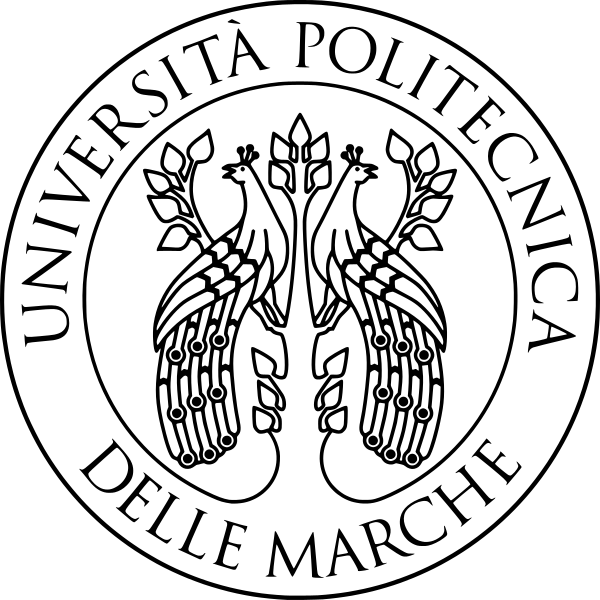
\includegraphics[width=15mm]{Immagini/univpmlogo}}
\titlegraphic{
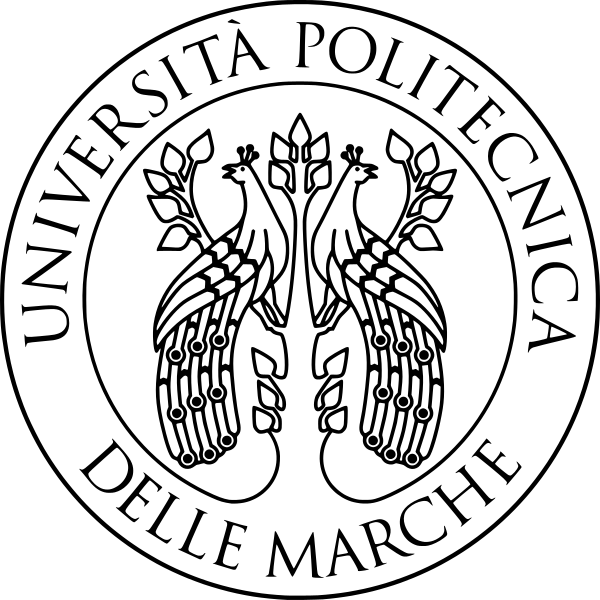
\includegraphics[width=2cm]{Immagini/univpmlogo}
}
\usepackage[english, italian]{babel} %l?ultima lingua dichiarata � la lingua principale del documento
\usepackage[latin1]{inputenc}
\usepackage[T1]{fontenc}
%\usepackage{subfig}
\usepackage{graphicx}
\usepackage{animate} %per le gif 
\usepackage{xcolor}
\usepackage{listings}
\usepackage{siunitx}
\usepackage{amssymb}
\usepackage{amsmath}
\usepackage{booktabs} %toprule, midrule, bottomrule
\usepackage{subcaption,booktabs}

\usetheme{Antibes}
\usecolortheme{default} %https://hartwork.org/beamer-theme-matrix/
%\useoutertheme[right,color=red]{sidebar} %{infolines}
%\setbeamertemplate{sidebar canvas right}[vertical shading][top=red,bottom=white]
\setbeamercovered{dynamic}

%\usepackage[latin1]{inputenc} %l'ho messo io (Jacopo)
%inizio impostazioni bibliografia
\usepackage[autostyle,italian=guillemets]{csquotes} 
%autostyle adatta lo stile delle citazioni alla lingua corrente del documento;
%italian=guillemets racchiude automaticamente tra virgolette caporali
%i campi che prevedono le virgolette;
\usepackage[backend=biber, style=numeric, citestyle=numeric,maxcitenames=2,maxbibnames = 2]{biblatex}
%backend=biber dice a biblatex che s?intende usare Biber come motore bibliografico
%style:numeric Anno di pubblicazione: in fondo al riferimento.
%citestyle=numeric Riferimento: numerico ([1], [2], eccetera).
%fine impostazioni bibliografia
\renewcommand*{\bibfont}{\footnotesize}

\addbibresource{Bibliografia.bib}

\begin{document}
	\begin{frame}
		\maketitle
	\end{frame}

\begin{frame}
	\frametitle{Contenuti}
	\tableofcontents
\end{frame}

\section{Introduzione}
\begin{frame}
\tableofcontents[currentsection]
\end{frame}

\begin{frame}
\frametitle{Cancellazione del crosstalk}
	\begin{block}{Obiettivo}
		Confrontare gli algoritmi LMS e Fast Deconvolution per la cancellazione del crosstalk.
	\end{block}
\begin{itemize}
\item Un sistema audio 3D permette
di posizionare i suoni intorno ad un ascoltatore in modo che questi siano
percepiti come provenienti da punti arbitrari nello spazio.
\item Se vengono utilizzati degli altoparlanti, la riproduzione di segnali binaurali all'orecchio dell'ascoltatore non � semplice. Ogni orecchio riceve una componente di diafonia, inoltre, i segnali diretti sono distorti dal riverbero della stanza. 
\item Per superare i problemi descritti sopra, � necessario un filtro
inverso prima di riprodurre il segnale binaurale attraverso gli altoparlanti.
\end{itemize}
\end{frame}

\begin{frame}
\begin{figure}[h]
	\centering	
	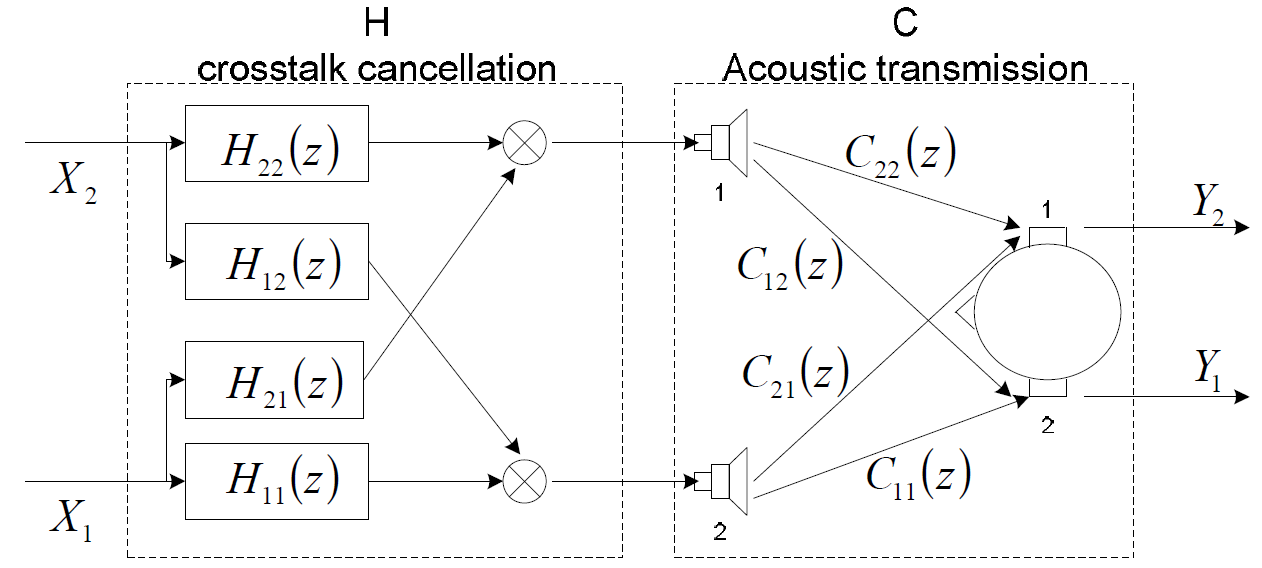
\includegraphics[width=\textwidth]{Immagini/head}
	\caption{Diagramma a blocchi del sistema sonoro usato}
	\label{fig:head}
\end{figure}
\end{frame}

\section{Stato dell'arte}
\begin{frame}
\tableofcontents[currentsection]
\end{frame}

\begin{frame}
\begin{itemize}
\item Supponendo che i percorsi di trasferimento acustico dagli altoparlanti alle
orecchie siano noti, il metodo di implementazione \textbf{diretto} calcola il filtro di cancellazione della diafonia invertendo le funzioni di trasferimento HRTF.
\item Nei metodi di implementazione \textbf{adattivi}, il filtro di cancellazione della diafonia � calcolato adattando i relativi coefficienti usando i segnali di feedback
ricevuti da microfoni in miniatura collocati nelle orecchie dell'utente.
\item I metodi diretti o adattativi possono essere implementati nel dominio del
\textbf{tempo} o della \textbf{frequenza}.
\item I primi sono generalmente
dispendiosi dal punto di vista computazionale, mentre i secondi hanno una
complessit� inferiore. Gli algoritmi nel dominio del tempo
hanno prestazioni migliori di quelli nel dominio della frequenza, data la stessa
lunghezza del filtro di cancellazione.
\end{itemize}

\end{frame}

\begin{frame}
\frametitle{Algoritmi nel dominio del tempo}
\begin{block}{LMS}
Noto per la sua
semplicit� e robustezza ed � ampiamente utilizzato, anche se la sua velocit�
di convergenza � lenta.
$$J=E[e[n]^2]=E[(d[n]-y[n])^2]$$
\end{block}

\begin{block}{RLS}
Si ottiene pesando in modo esponenziale i dati in modo da rimuovere
gradualmente gli effetti dei vecchi dati sui coefficienti del filtro e permettere il tracciamento di segnali che variano lentamente. $$J(\mathbf{h}_n) = \sum_{i = 0}^{n} \lambda^{n-i}e^2[i]$$
\end{block}

\end{frame}	
\begin{frame}
\frametitle{Algoritmi nel dominio della frequenza}
\begin{block}{Fast Deconvolution}
La Fast Deconvolution � un metodo molto veloce per calcolare una matrice
di filtri digitali che pu� essere utilizzata per controllare le uscite di un
impianto multicanale.
$$J = E + \beta V(f)$$
\end{block}

\begin{block}{FLMS}
Un algoritmo derivato da LMS � FLMS (Fast Least Mean Square), viene implementato nel dominio della frequenza e richiede uno sforzo computazionale minore rispetto alla sua controparte nel dominio
del tempo.
\end{block}
\end{frame}	
	
\section{Dataset}
\begin{frame}
\tableofcontents[currentsection]
\end{frame}

\begin{frame}
\frametitle{Dataset utilizzato}
\begin{block}{HRTF Measurements of a KEMAR Dummy-Head Microphone}%~\cite{Gardner:HRTF}
\begin{itemize}
\item Dataset del MIT.
\item Risposte impulsive dell'orecchio sinistro
e destro rispetto ad un altoparlante Realistic Optimus Pro 7 montato a 1,4 metri dal
KEMAR.
\item I dati HRTF vengono archiviati nelle directory per elevazione. Ogni nome
di directory ha il formato ``elevEE'', dove ``EE'' � l'angolo di elevazione.
\item All'interno
di ogni directory, il nome di ogni file ha il formato ``XEEeAAAa.wav''
dove X pu� essere ``L'' o ``R'' rispettivamente per la risposta dell'orecchio
sinistro e destro e ``AAA'' � l'azimut della sorgente in gradi, da 0� a 355�.
\end{itemize}
\end{block}
\end{frame}	

\section{LMS}
\begin{frame}[allowframebreaks]
\tableofcontents[currentsection]
\end{frame}

\begin{frame}[allowframebreaks]
In generale, si pu� scrivere l'uscita $y[n]$ del filtraggio nell'$n$-esimo istante di un segnale $\mathbf{a[n]}$ definito come:
\begin{equation*}
\mathbf{a[n]} = \left[a[n], a[n-1], \dots, a[n - M + 1]\right]^T
\end{equation*}
con un filtro $\mathbf{b[n]}$ di lunghezza $M$ con coefficienti del tipo:
\begin{equation*}
\mathbf{b[n]} =  \left[b_{0}[n], b_{1}[n], \dots, b_{M-1}[n]\right]^T
\end{equation*}
come:
\begin{equation}\label{eq:filtraggio_prodotto_scalare}
y[n] = \sum_{j=0}^{M-1}b_{j}[n]a[n-j] = \mathbf{b}^T[\mathbf{n}] \cdot \mathbf{a}[\mathbf{n}].
\end{equation}

Il filtraggio dei segnali di riferimento $x_i[n]$ con le hrir $c_{lm}$ � dato dalla seguente equazione:
\begin{equation}\label{eq:r_ilm}
r_{ilm}[n]=\sum_{j=0}^{M-1}c_{lm}[j]x_i[n-j].
\end{equation}

Si pu� applicare la formula~\eqref{eq:filtraggio_prodotto_scalare} all'equazione~\eqref{eq:r_ilm} per calcolare le $r_{ilm}[n]$ nel seguente modo:

\begin{equation}\label{eq:r_ilm_prodotto_scalare}
r_{ilm}[n]=\sum_{j=0}^{M-1}c_{lm,j}[n]x_i[n-j] = \mathbf{c_{lm}}^T[\mathbf{n}] \cdot \mathbf{x_i}[\mathbf{n}].
\end{equation}

Il segnale ricevuto ad ogni orecchio � dato da:
\begin{equation}\label{eq:y_i_lms}
y_i[n]=r_{1i1}[n] \circledast h_{11}[n]+r_{1i2}[n] \circledast h_{21}[n]+
r_{2i1}[n] \circledast h_{12}[n]+r_{2i2}[n] \circledast h_{22}[n].
\end{equation}
Il criterio dell'algoritmo LMS � la minimizzazione della funzione costo
\begin{equation}\label{eq:errore_lms}
J=E[e[n]^2]=E[(d[n]-y[n])^2]
\end{equation}
dove $e[n]$, $d[n]$ e $y[n]$ sono definiti come:
\begin{equation}
e[n]=
\begin{bmatrix}
e_1[n]\\
e_2[n]
\end{bmatrix},\quad
d[n]=
\begin{bmatrix}
d_1[n]\\
d_2[n]
\end{bmatrix},\quad
y[n]=
\begin{bmatrix}
y_1[n]\\
y_2[n]
\end{bmatrix}.
\end{equation}
La minimizzazione di $J$ avviene con il metodo steepest descend e l'aggiornamento dei tappi del filtro adattativo segue la formula:
\begin{equation}\label{eq:aggiornamento_lms}
h^{(k+1)} = h^{(k)} - \mu e_i^{(k)} \cdot \mathbf{r}_i^T.
\end{equation}
Esplicitando l'equazione~\eqref{eq:aggiornamento_lms} per il primo canale, si ottiene:
\[
\begin{split}
h_{11}^{(k+1)}[n] \leftarrow h_{11}^{(k)}[n] - \mu e_1^{(1)} \cdot r_{111}[n]\\
h_{21}^{(k+1)}[n] \leftarrow h_{21}^{(k)}[n] - \mu e_1^{(1)} \cdot r_{112}[n]\\
h_{12}^{(k+1)}[n] \leftarrow h_{12}^{(k)}[n] - \mu e_1^{(1)} \cdot r_{211}[n]\\
h_{22}^{(k+1)}[n] \leftarrow h_{22}^{(k)}[n] - \mu e_1^{(1)} \cdot r_{212}[n]
\end{split}
\]
L'aggiornamento usando il secondo canale avviene in modo analogo.
\end{frame}

\begin{frame}
\begin{figure}[h]
	\centering	
	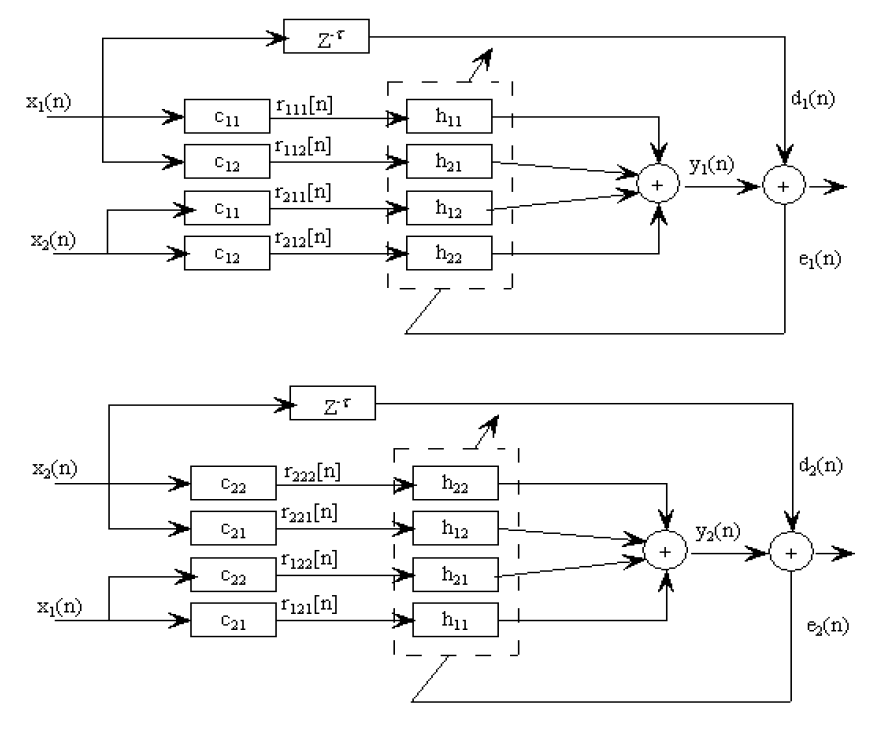
\includegraphics[width=0.6\textwidth]{Immagini/lms}
	\caption{Diagramma a blocchi della cancellazione del crosstalk usando LMS}
	\label{fig:lms}
\end{figure}
\end{frame}

\section{Fast Deconvolution}
\begin{frame}
\tableofcontents[currentsection]
\end{frame}

\begin{frame}[allowframebreaks]
\begin{block}{Deconvoluzione}
La deconvoluzione, nella sua forma pi� elementare, pu� essere descritta come il compito di calcolare l'input di un sistema a tempo discreto conoscendo il suo output. 
%Di solito si presume che il sistema sia lineare e che la relazione input output sia nota con precisione. 
\end{block}
Consideriamo una funzione costo del tipo:
\begin{equation}\label{eq:funzione_costo_fd}
J = E + \beta V(f)
\end{equation}
dove $E$ � una misura dell'errore della pressione sonora:
\begin{equation}\label{eq:errore_fd}
E = | Y_1 - X_1 |^2  + | Y_2 - X_2 |^2
\end{equation}
e $V$ � una funzione della frequenza che indica il costo computazionale. Il numero $\beta \geq 0$ � un parametro di regolarizzazione che determina quanto peso
assegnare alla funzione $V(f)$.

Siano $S$ i segnali trasferiti agli altoparlanti facendo passare il segnale $X$ attraverso la matrice di cancellazione del crosstalk $H$. Otteniamo:
\begin{equation}
V(f) = S_b ^{+} S_b
\end{equation}
con
\begin{equation}
S_b = BS = BHX,
\end{equation}
dove $B$ � una matrice $2 \times 2$ e il simbolo $^+$ indica l'inversa generalizzata della matrice $S_b$. 
%La soluzione approssimata della funzione $J$ � definita da:
%\begin{equation}\label{eq:H_FD}
%H(z) = \left[C^T (z^{-1}) C(z) + \beta B^T B)\right]^{-1} C^T(z^{-1}).
%\end{equation}
%Se la matrice $B$ � uguale alla matrice identit� $I$, si ottiene $S_b = S$, %dunque l'equazione~\eqref{eq:H_FD} diventa:
%\begin{equation}\label{eq:H_FD2}
%H(z) = \left[C^T (z^{-1}) C(z) + \beta I)\right]^{-1} C^T(z^{-1}) z^{-m}
%\end{equation}
%dove la componente $z^{-m}$ implementa un ritardo di $m$ campioni. 
%Un ritardo di modellazione viene utilizzato per garantire che la rete di cancellazione del cross-talk funzioni bene non solo in termini di ampiezza, ma anche in termini di fase.
%Le equazioni~\eqref{eq:H_FD} e~\eqref{eq:H_FD2} rappresentano una espressione di $H(z)$ nel dominio continuo della frequenza. 
Se, come nel nostro caso, il dominio della frequenza � discreto e $B = I$, la soluzione approssimata della funzione $J$ � definita da:
\begin{equation}\label{eq:H_FD3}
H[k] = \left[C^H[k] C[k] + \beta I)\right]^{-1} C^H[k]
\end{equation}
dove $k$ indica la $k$-esima frequenza corrispondente a $\exp(j2\pi k/N)$ e l'apice~$^H$ denota l'operatore Hermitiano. 

%Dall'equazione~\eqref{eq:H_FD3} si pu� osservare che ponendo $\beta = 0$ si ottiene $H = C^{-1}$. In questo caso, poich� $Y = CHX = C C^{-1} X = IX = X$, si ottiene in uscita il segnale d'ingresso.
\end{frame}

\begin{frame}[allowframebreaks]{Overlap and Save}
Dato che l'uscita $Y$ � data da:
\begin{equation}\label{eq:y_matrix}
Y = CHX = 
\begin{bmatrix}
C_{11} X_1 & C_{12} X_1 & C_{11} X_2 & C_{12} X_2 \\ 
C_{21} X_1 & C_{22} X_1 & C_{21} X_2 & C_{22} X_2 \\ 
\end{bmatrix}
\begin{bmatrix}
H_{11}\\
H_{21}\\
H_{12}\\
H_{22}\\
\end{bmatrix},
\end{equation}
nell'implementazione pratica non si pu� calcolare tutta l'uscita con la sola operazione matriciale~\eqref{eq:y_matrix}, occorre usare la tecnica dell'overlap and save per filtrare l'ingresso $X$ con i filtri $C$ e $H$. L'overlap and save � utile per eseguire un filtraggio in real time con un filtro a risposta impulsiva finita.

\begin{figure}[h]
	\centering	
	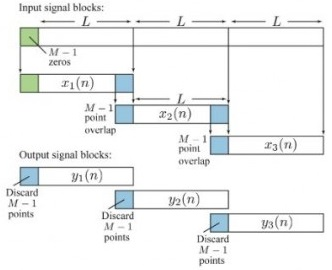
\includegraphics[width=.6\textwidth]{Immagini/ols}
	\caption{Metodo Overlap and Save}
	\label{fig:ols}
\end{figure}

\end{frame}

\section{Implementazione NU-Tech}
\begin{frame}
\tableofcontents[currentsection]
\end{frame}

\begin{frame}{LMS}
\begin{enumerate}
\item Inizializzazione delle variabili nel costruttore.
\item Allocazione delle variabili e lettura delle HRIR nella Init.
\item Costruzione segnale desiderato traslando il segnale di ingresso di $\tau$ campioni nella Process.
\item Filtraggio dei segnali $x_i[n]$ con le HRIR $c_{lm}$ usando l'equazione~\eqref{eq:r_ilm_prodotto_scalare}.
\item Calcolo delle uscite con la formula~\eqref{eq:y_i_lms}.
\item Calcolo dell'errore come la differenza fra il segnale desiderato e l'uscita effettiva.
\item Aggiornamento dei tappi del filtro di ricostruzione con la formula~\eqref{eq:aggiornamento_lms}.
\item Deallocazione della memoria nella Delete.
\end{enumerate}
\end{frame}

\begin{frame}{Fast Deconvolution}
\begin{enumerate}
\item Inizializzazione delle variabili nel costruttore.
\item Allocazione delle variabili e lettura delle HRIR nella Init.
\item Calcolo della FFT a fftLen punti delle HRIR.
\item Calcolo della matrice $\mathbf{H}$ con la formula~\eqref{eq:H_FD3}.
\item Costruzione del buffer di ingresso con $f_s$ campioni per l'overlap and save nella Process.
\item Calcolo della FFT a fftLen punti del buffer di ingresso.
\item Calcolo del buffer di uscita moltiplicando il buffer di ingresso per le HRTF.
\item Aggiornamento dell'uscita scartando i primi $f_s$ campioni del buffer.
\item Deallocazione della memoria nella Delete.
\end{enumerate} 
\end{frame}

\section{Risultati}
\begin{frame}
\tableofcontents[currentsection]
\end{frame}

\begin{frame}{Risultati Matlab}
\begin{block}{Fattori di separazione dei canali}
\begin{equation}\label{eq:JL}
J_L = E\left\{20\cdot\log_{10} \dfrac{C_{11}H_{11}+C_{12}H_{21}}{C_{21}H_{11}+C_{22}H_{21}}\right\} \quad [\si{\decibel}]
\end{equation}

\begin{equation}\label{eq:JR}
J_R = E\left\{20\cdot\log_{10} \dfrac{C_{22}H_{22}+C_{21}H_{12}}{C_{12}H_{22}+C_{11}H_{12}}\right\} \quad [\si{\decibel}]
\end{equation}
\end{block}
\end{frame}

\begin{frame}
\begin{table}[h]
    \begin{subtable}{.4\linewidth}
      \centering
        \begin{tabular}{c c c}
        \toprule
        $\mu$   & $J_R$ [\si{\decibel}]   & $J_L$ [\si{\decibel}]   \\ \midrule
        $10^{-3}$ & 22.032 & 21.924 \\
        $5\cdot10^{-4}$ & 17.610 & 20.375 \\
        $10^{-4}$& 11.063 & 16.921 \\
        $5\cdot10^{-5}$ & 9.742  & 16.161 \\ \bottomrule
        \end{tabular}
        \caption{\label{tab:LMS_result}Confronto di $J_R$ e $J_L$ per l'algoritmo LMS per diversi $\mu$.}
    \end{subtable}
    \hfill
    \begin{subtable}{.4\linewidth}
      \centering
        \begin{tabular}{c c c}
        \toprule
		$\beta$   & $J_R$ [\si{\decibel}]   & $J_L$ [\si{\decibel}]   \\ \midrule
		$1$ &  25.062 &  26.538\\
		$0.3$ &  28.829 &  30.498\\
		$0.1$&  34.908 & 36.532 \\
		$0.01$ &  47.657 &  48.661 \\ \bottomrule
        \end{tabular}
		\caption{\label{tab:FD_result}Confronto di $J_R$ e $J_L$ per l'algoritmo FD per diversi $\beta$.}
    \end{subtable} 
    \vfill
     \begin{subtable}{.4\linewidth}
          \centering
            \begin{tabular}{c c c}
            \toprule
            Azimuth  & $J_R$ [\si{\decibel}]   & $J_L$ [\si{\decibel}]   \\ \midrule
            $\pm \SI{20}{\degree}$ & 21.511 & 25.532\\
            $\pm \SI{30}{\degree}$ & 22.032 & 21.924  \\
            $\pm \SI{40}{\degree}$ & 19.667 & 23.528 \\ \bottomrule
            \end{tabular}
            \caption{\label{tab:LMS_result_azimuth}Confronto di $J_R$ e $J_L$ per l'algoritmo LMS per diversi angoli azimutali con $\mu = 10^{-3}$.}
    \end{subtable}
 	\hfill 
     \begin{subtable}{.4\linewidth}
        \centering
          \begin{tabular}{c c c}
          \toprule
          Azimuth  & $J_R$ [\si{\decibel}]   & $J_L$ [\si{\decibel}]   \\ \midrule
          $\pm \SI{20}{\degree}$ &  45.672 &  47.034\\
          $\pm \SI{30}{\degree}$ &  34.908 & 36.532 \\
          $\pm \SI{40}{\degree}$ &  40.523 &  42.098\\ \bottomrule
          \end{tabular}
          \caption{\label{tab:FD_result_azimuth}Confronto di $J_R$ e $J_L$ per l'algoritmo FD per diversi angoli azimutali con $\beta = 0.1$.}
      \end{subtable}
\end{table}
\end{frame}

\begin{frame}
\begin{figure}[h]
\begin{subfigure}{.45\textwidth}
	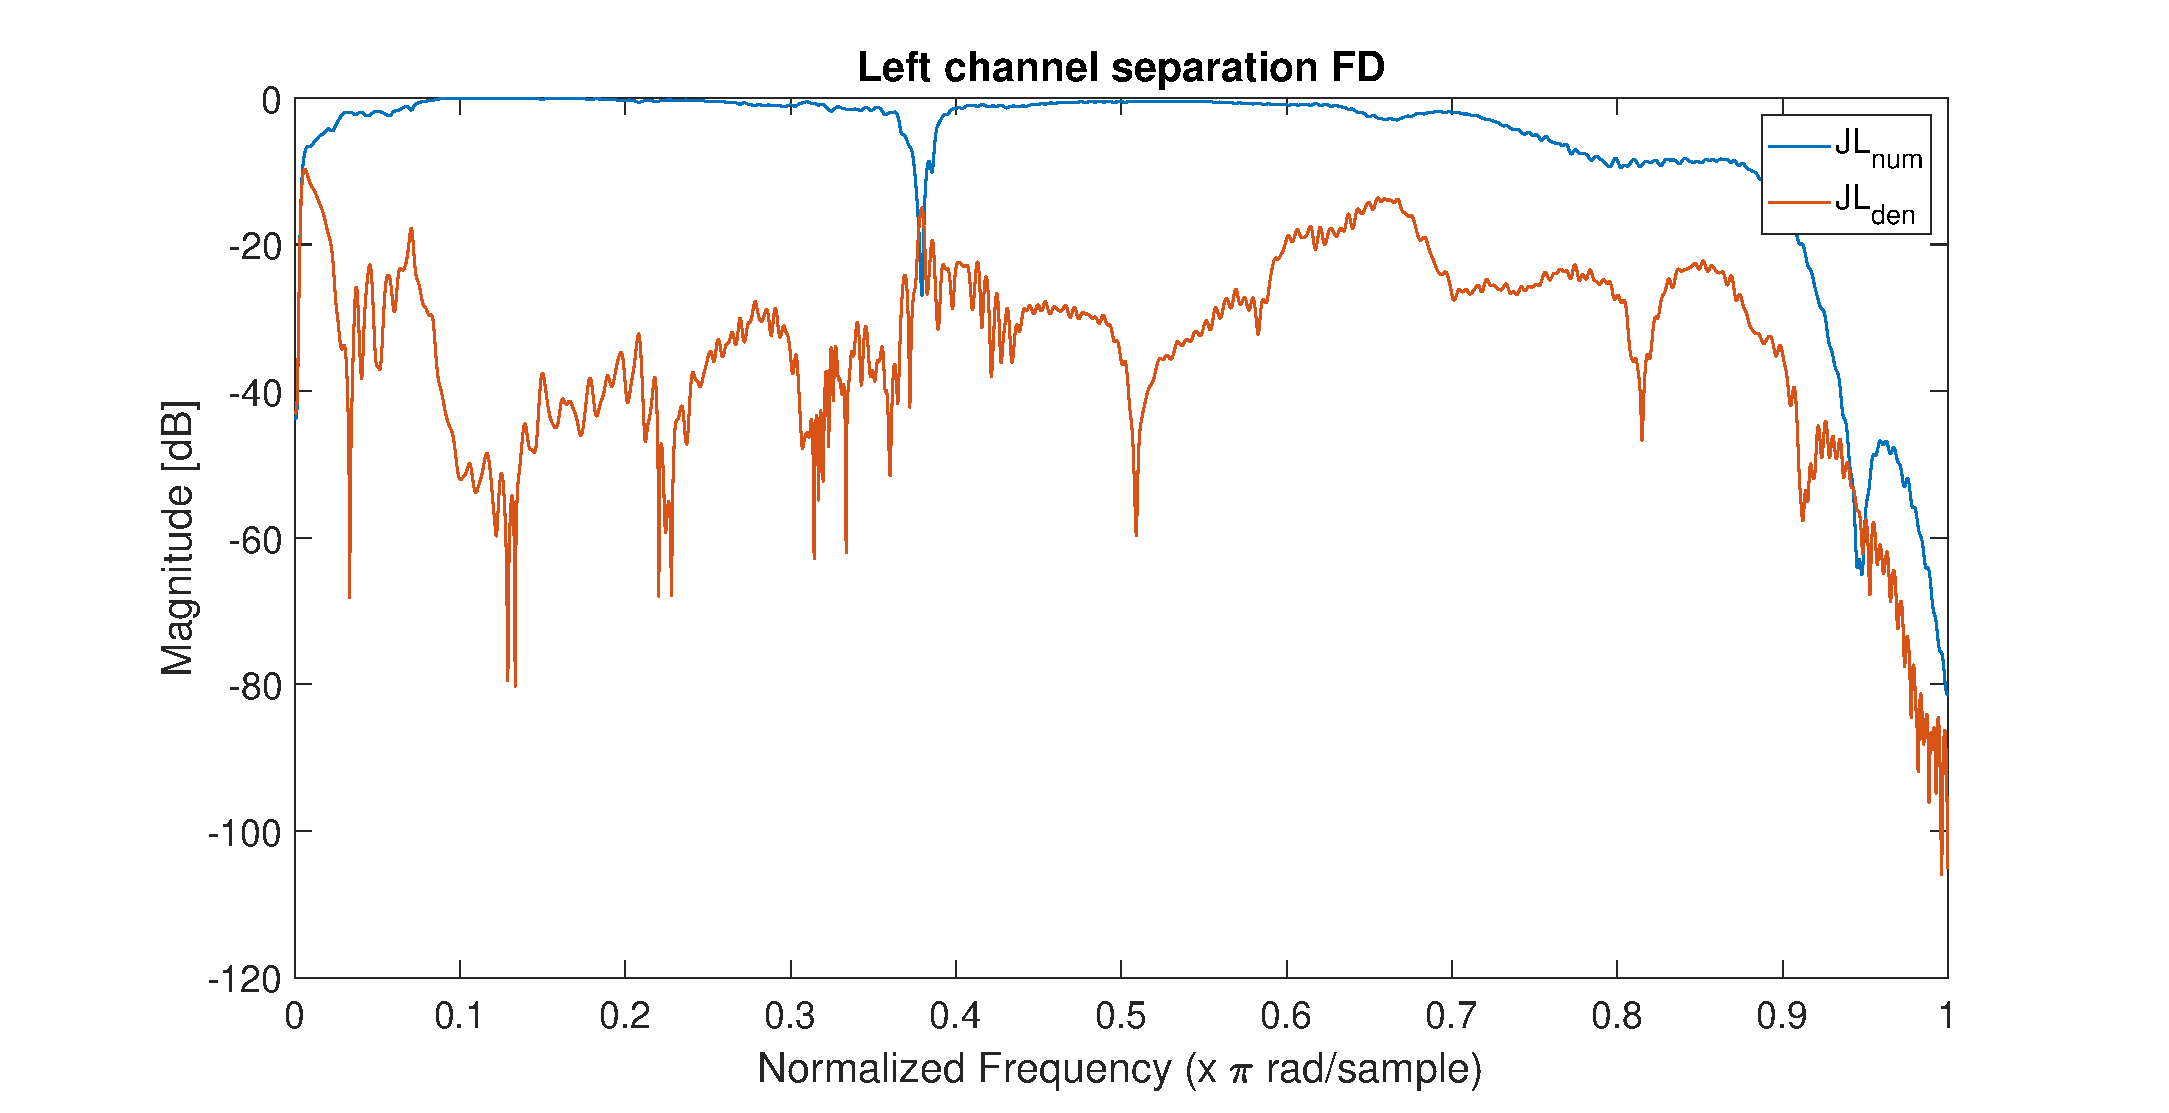
\includegraphics[width=1\textwidth]{Immagini/left_channel_separation_FD}
	\caption{}
	\label{left_channel_separation_FD}
\end{subfigure}
\hfill
\begin{subfigure}{.45\textwidth}
	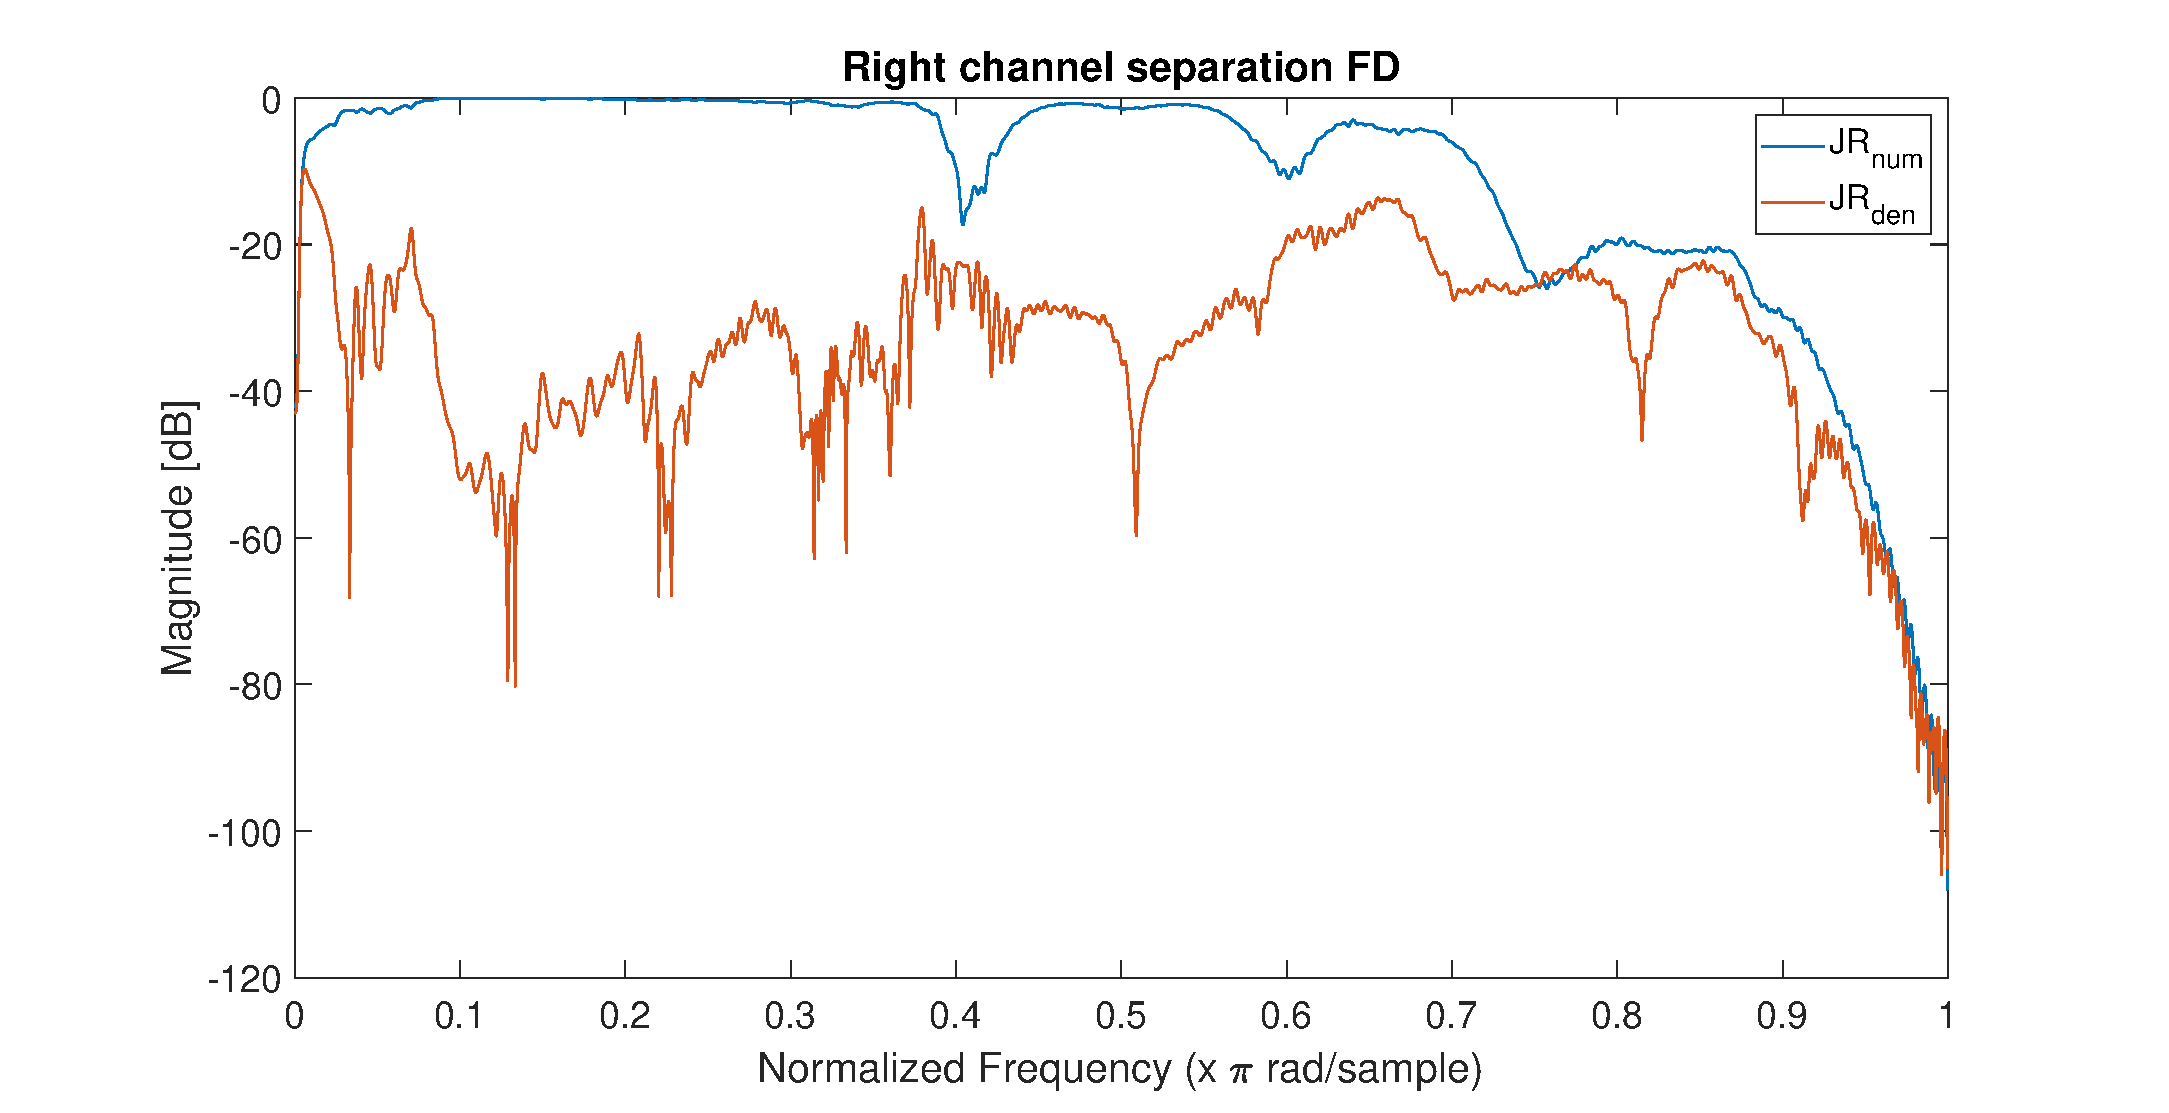
\includegraphics[width=1\textwidth]{Immagini/right_channel_separation_FD}
	\caption{}
	\label{right_channel_separation_FD}
\end{subfigure}
\vfill
\begin{subfigure}{.45\textwidth}
	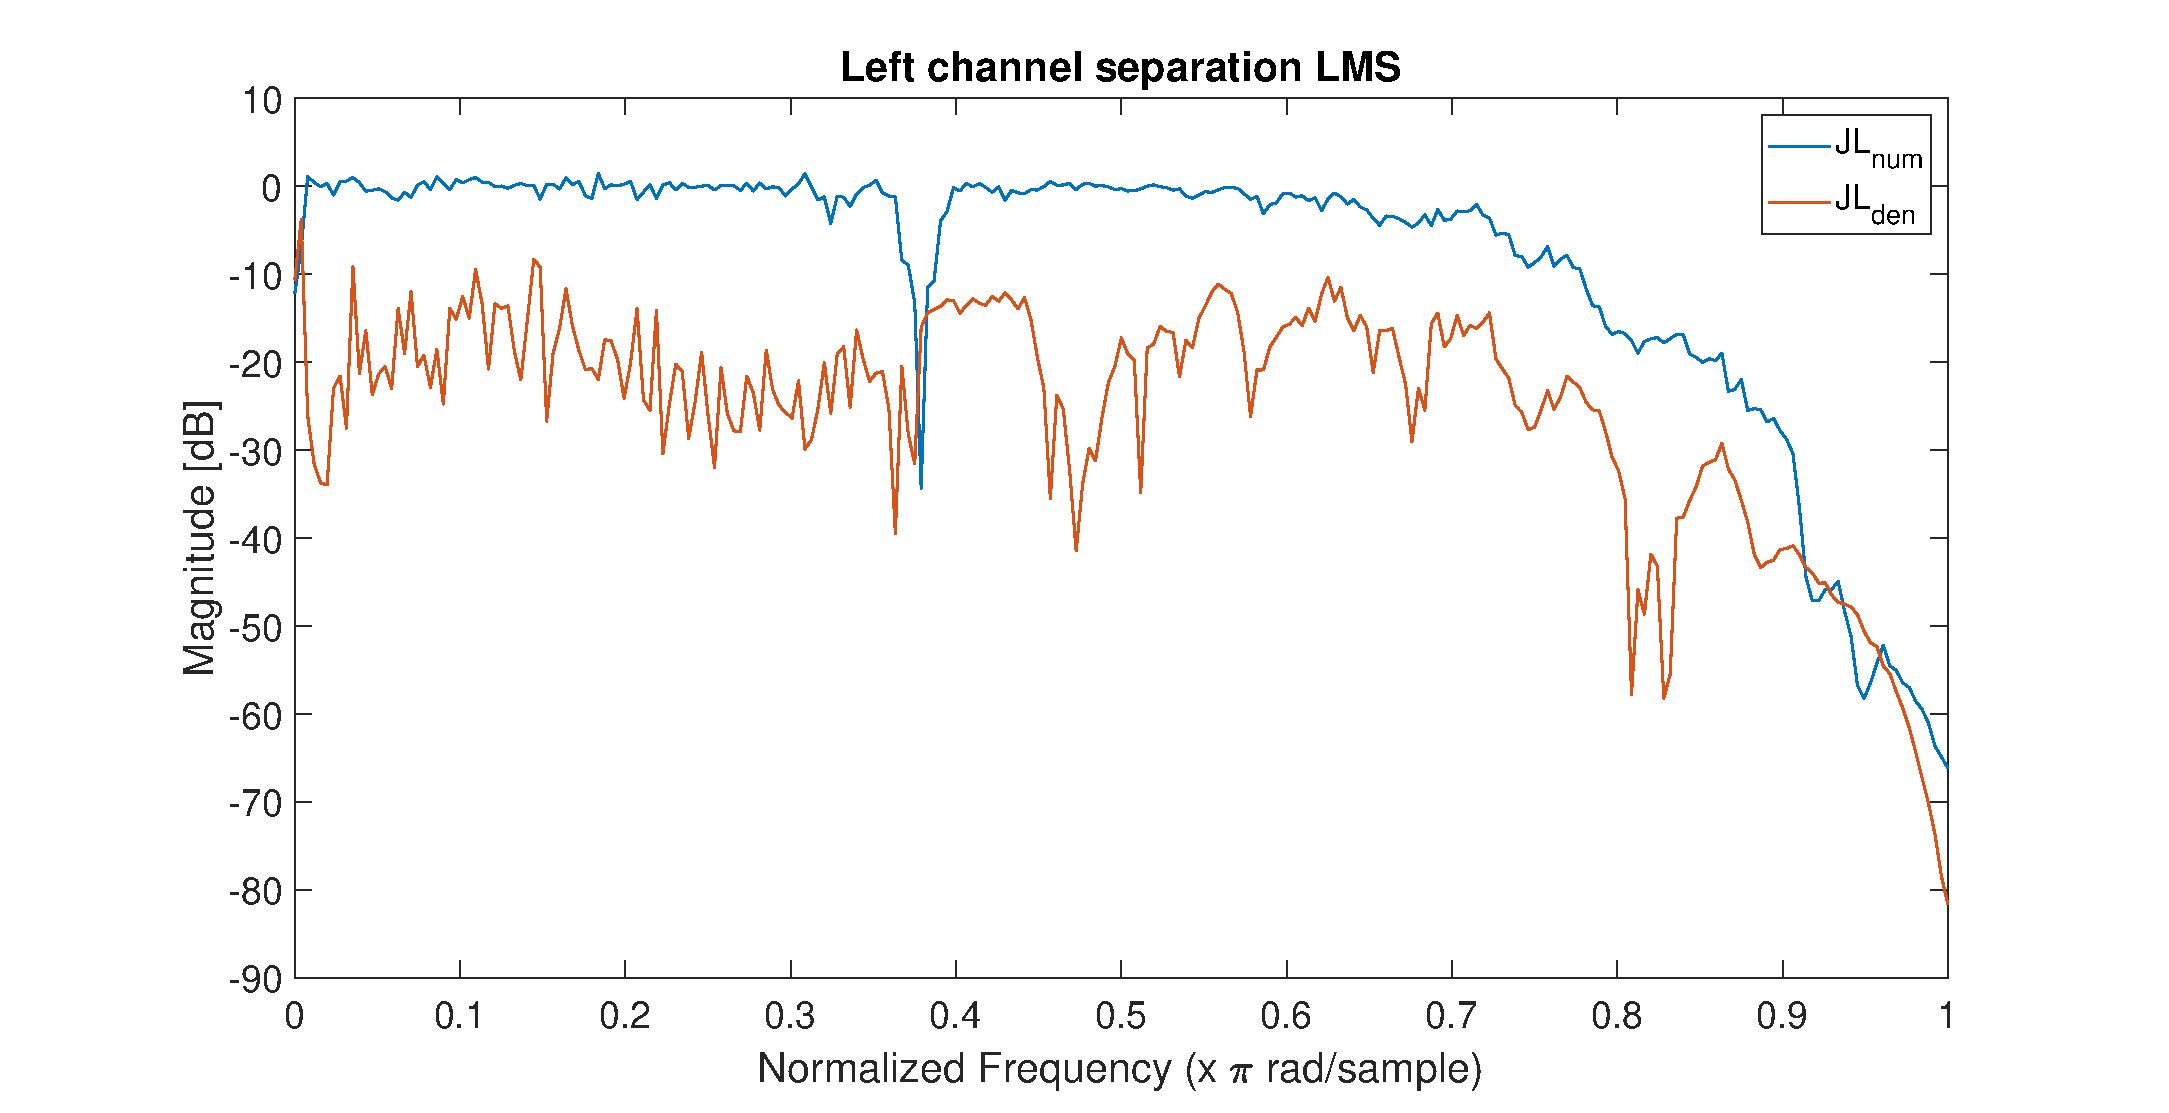
\includegraphics[width=1\textwidth]{Immagini/left_channel_separation_LMS}
	\caption{}
	\label{left_channel_separation_LMS}
\end{subfigure}
\hfill
\begin{subfigure}{.45\textwidth}
	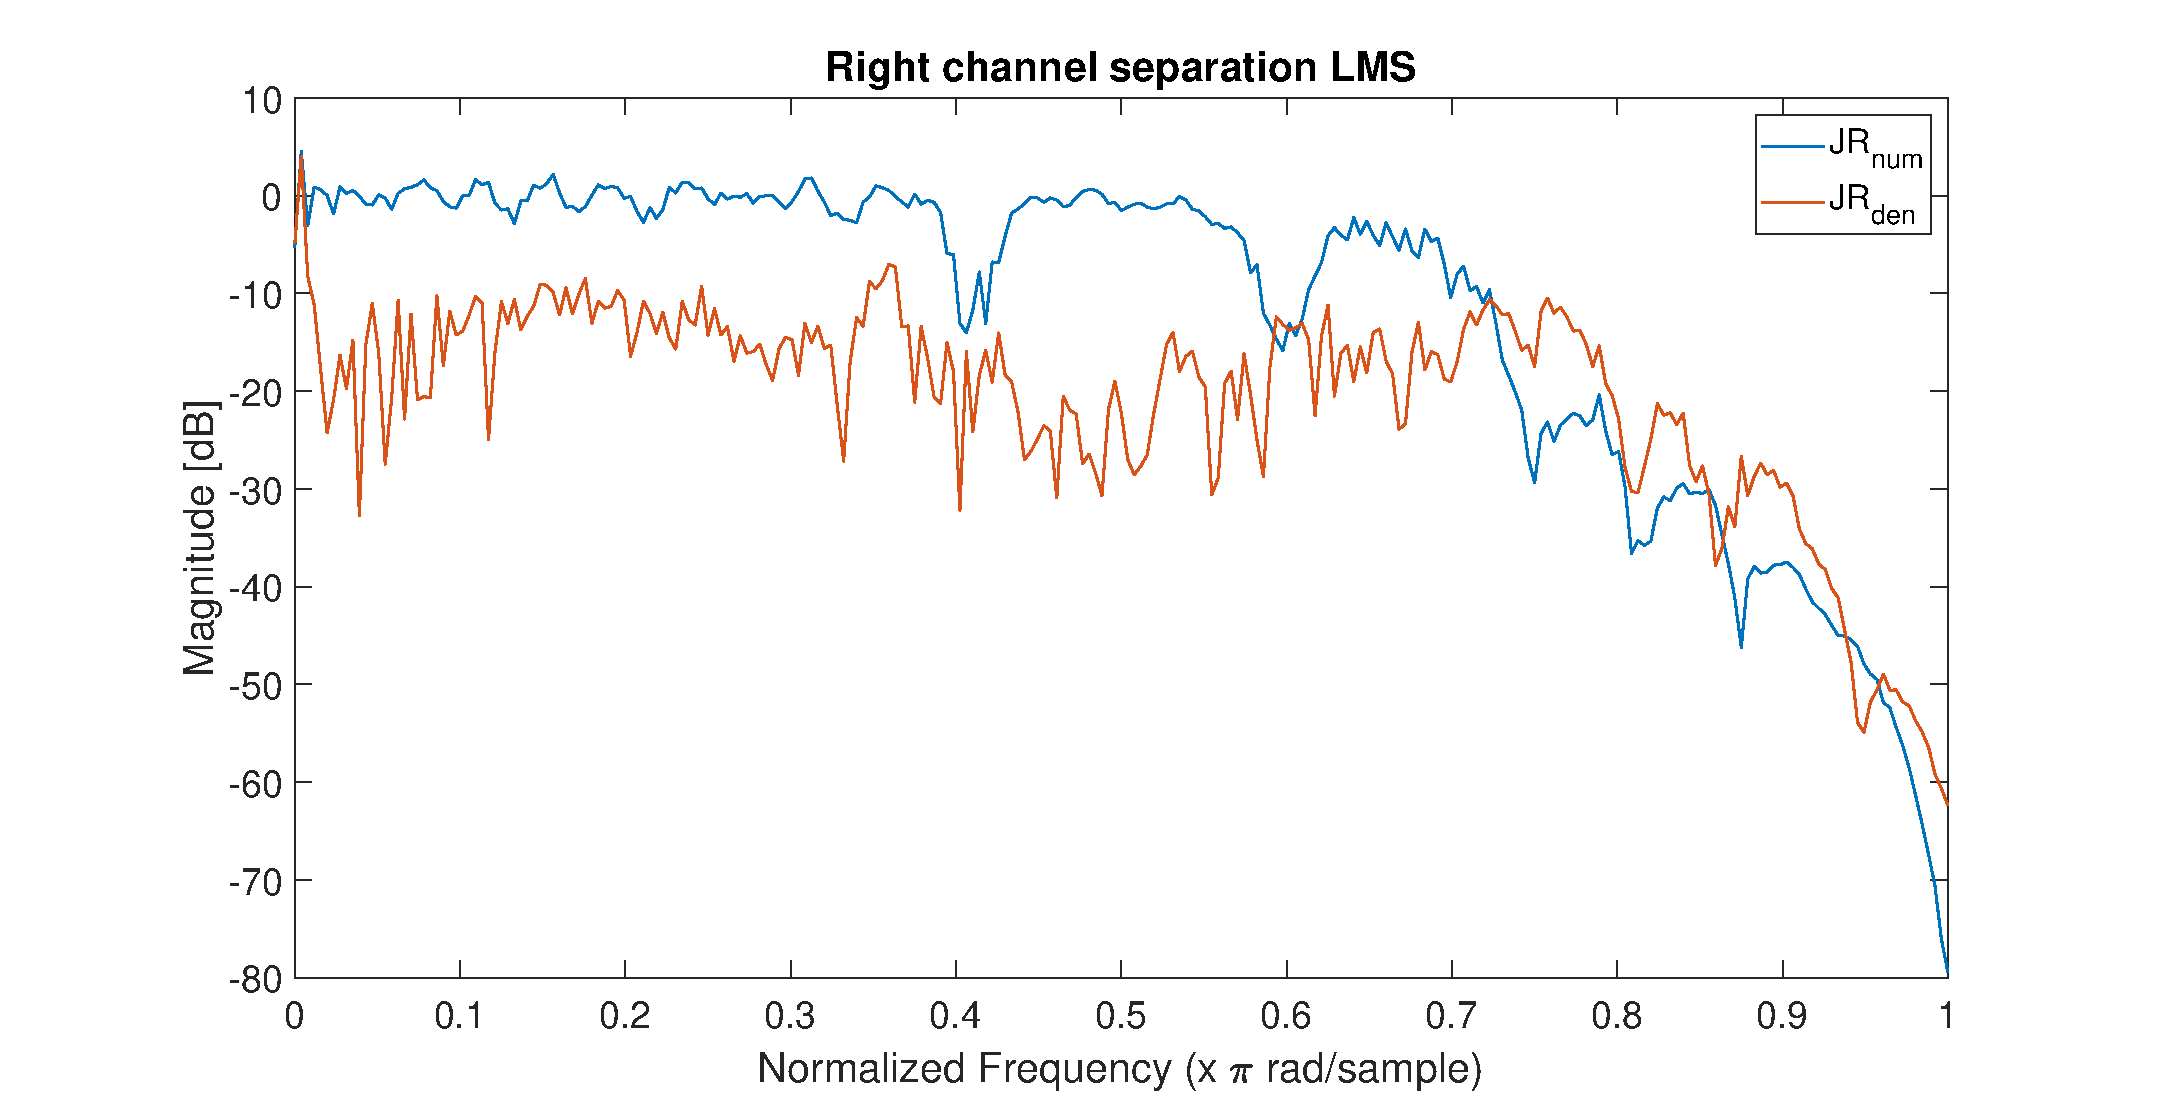
\includegraphics[width=1\textwidth]{Immagini/right_channel_separation_LMS}
	\caption{}
	\label{right_channel_separation_LMS}
\end{subfigure}
\caption{Confronto del numeratore e del denominatore di (a) $J_L$ e (b) $J_R$ per FD con $\beta = 0.3$, (c) $J_L$ e (d) $J_R$ per LMS con $\mu = 10^{-3}$.}
\label{fig:channel_separation_LMS_FD}
\end{figure}
\end{frame}

\begin{frame}
\begin{figure}[h]
	\begin{subfigure}{.45\textwidth}
		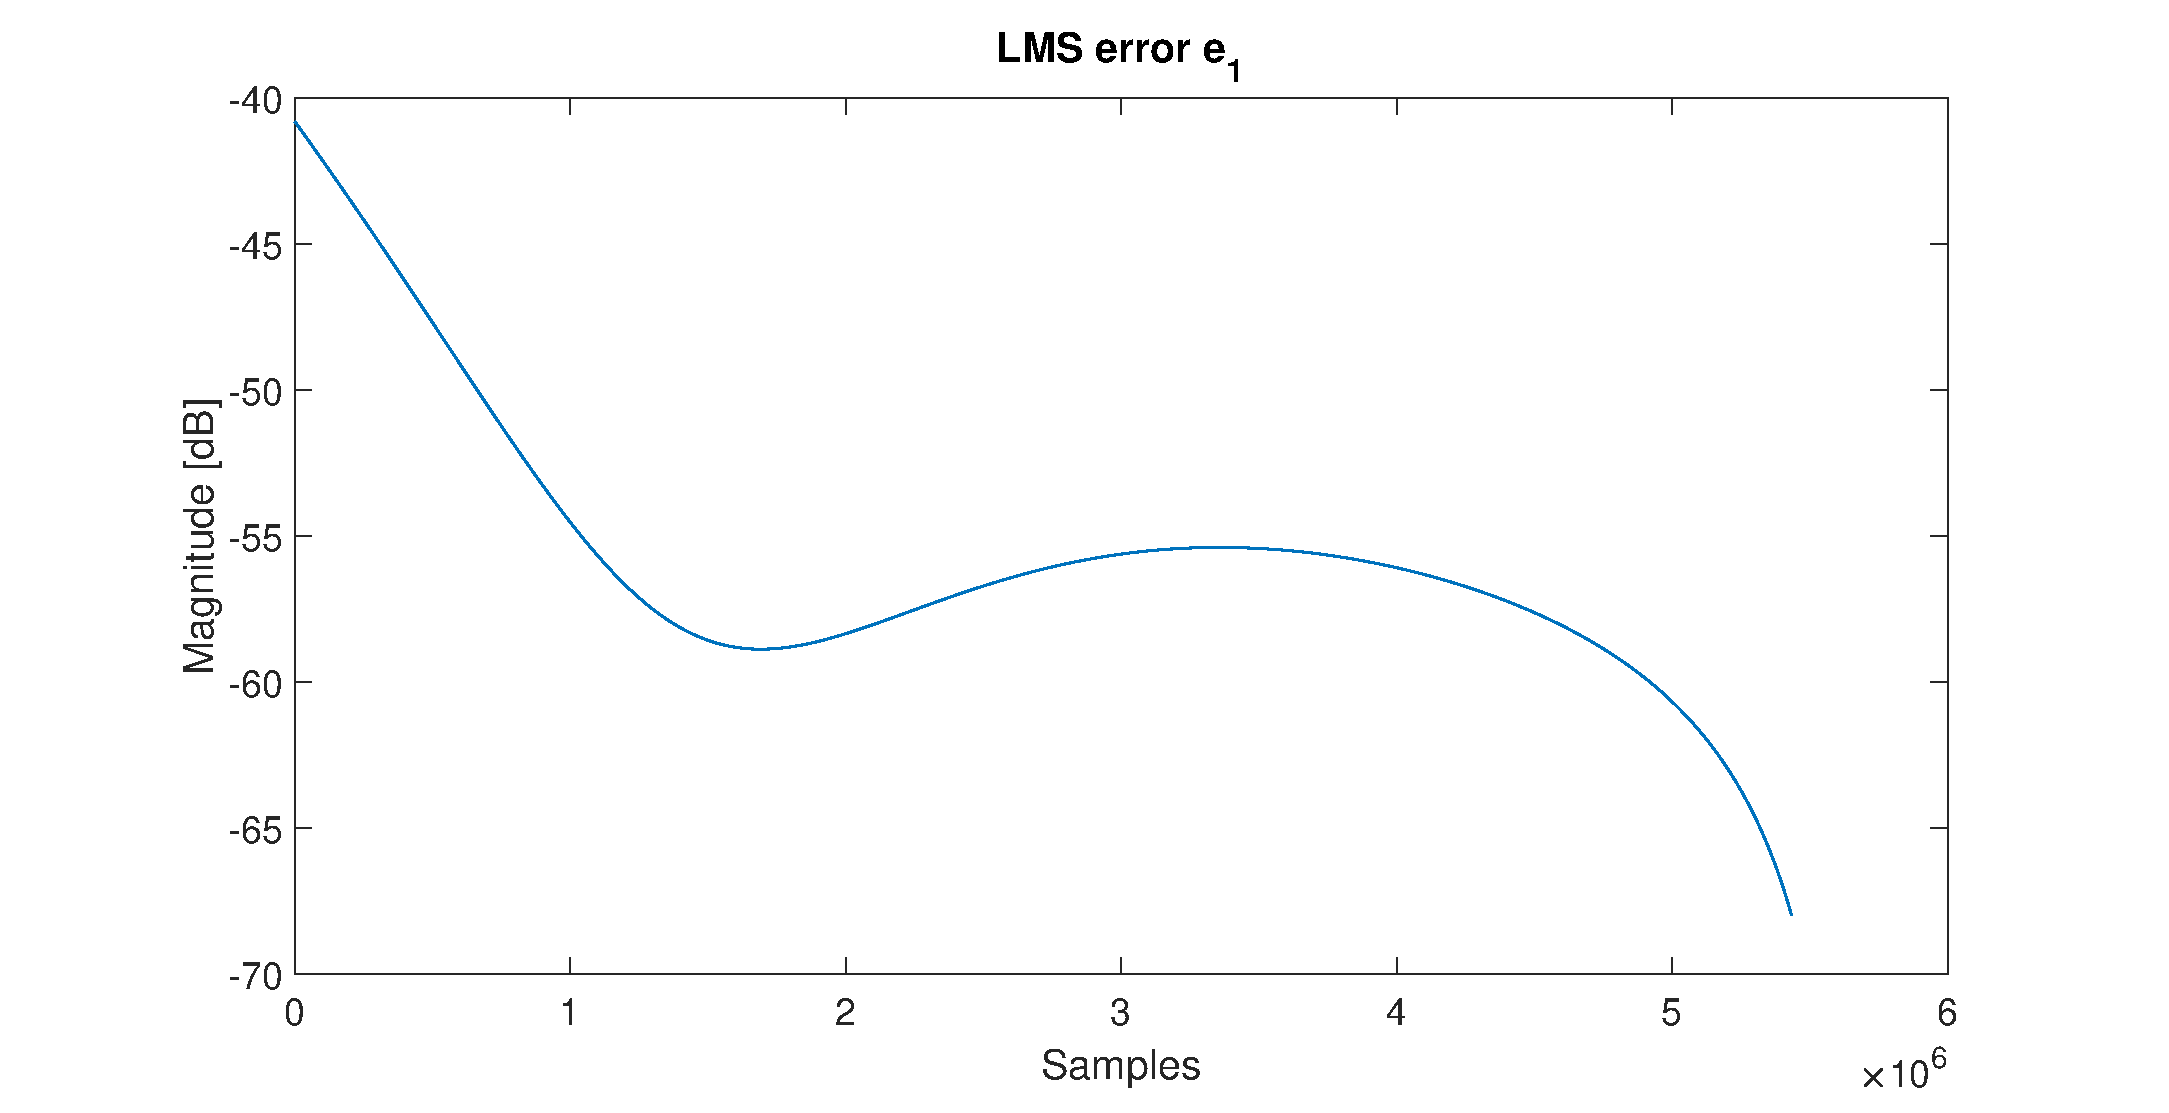
\includegraphics[width=1\textwidth]{Immagini/mse_e1}
		\caption{}
		\label{mse_e1}
	\end{subfigure}
	\vfill
	\begin{subfigure}{.45\textwidth}
		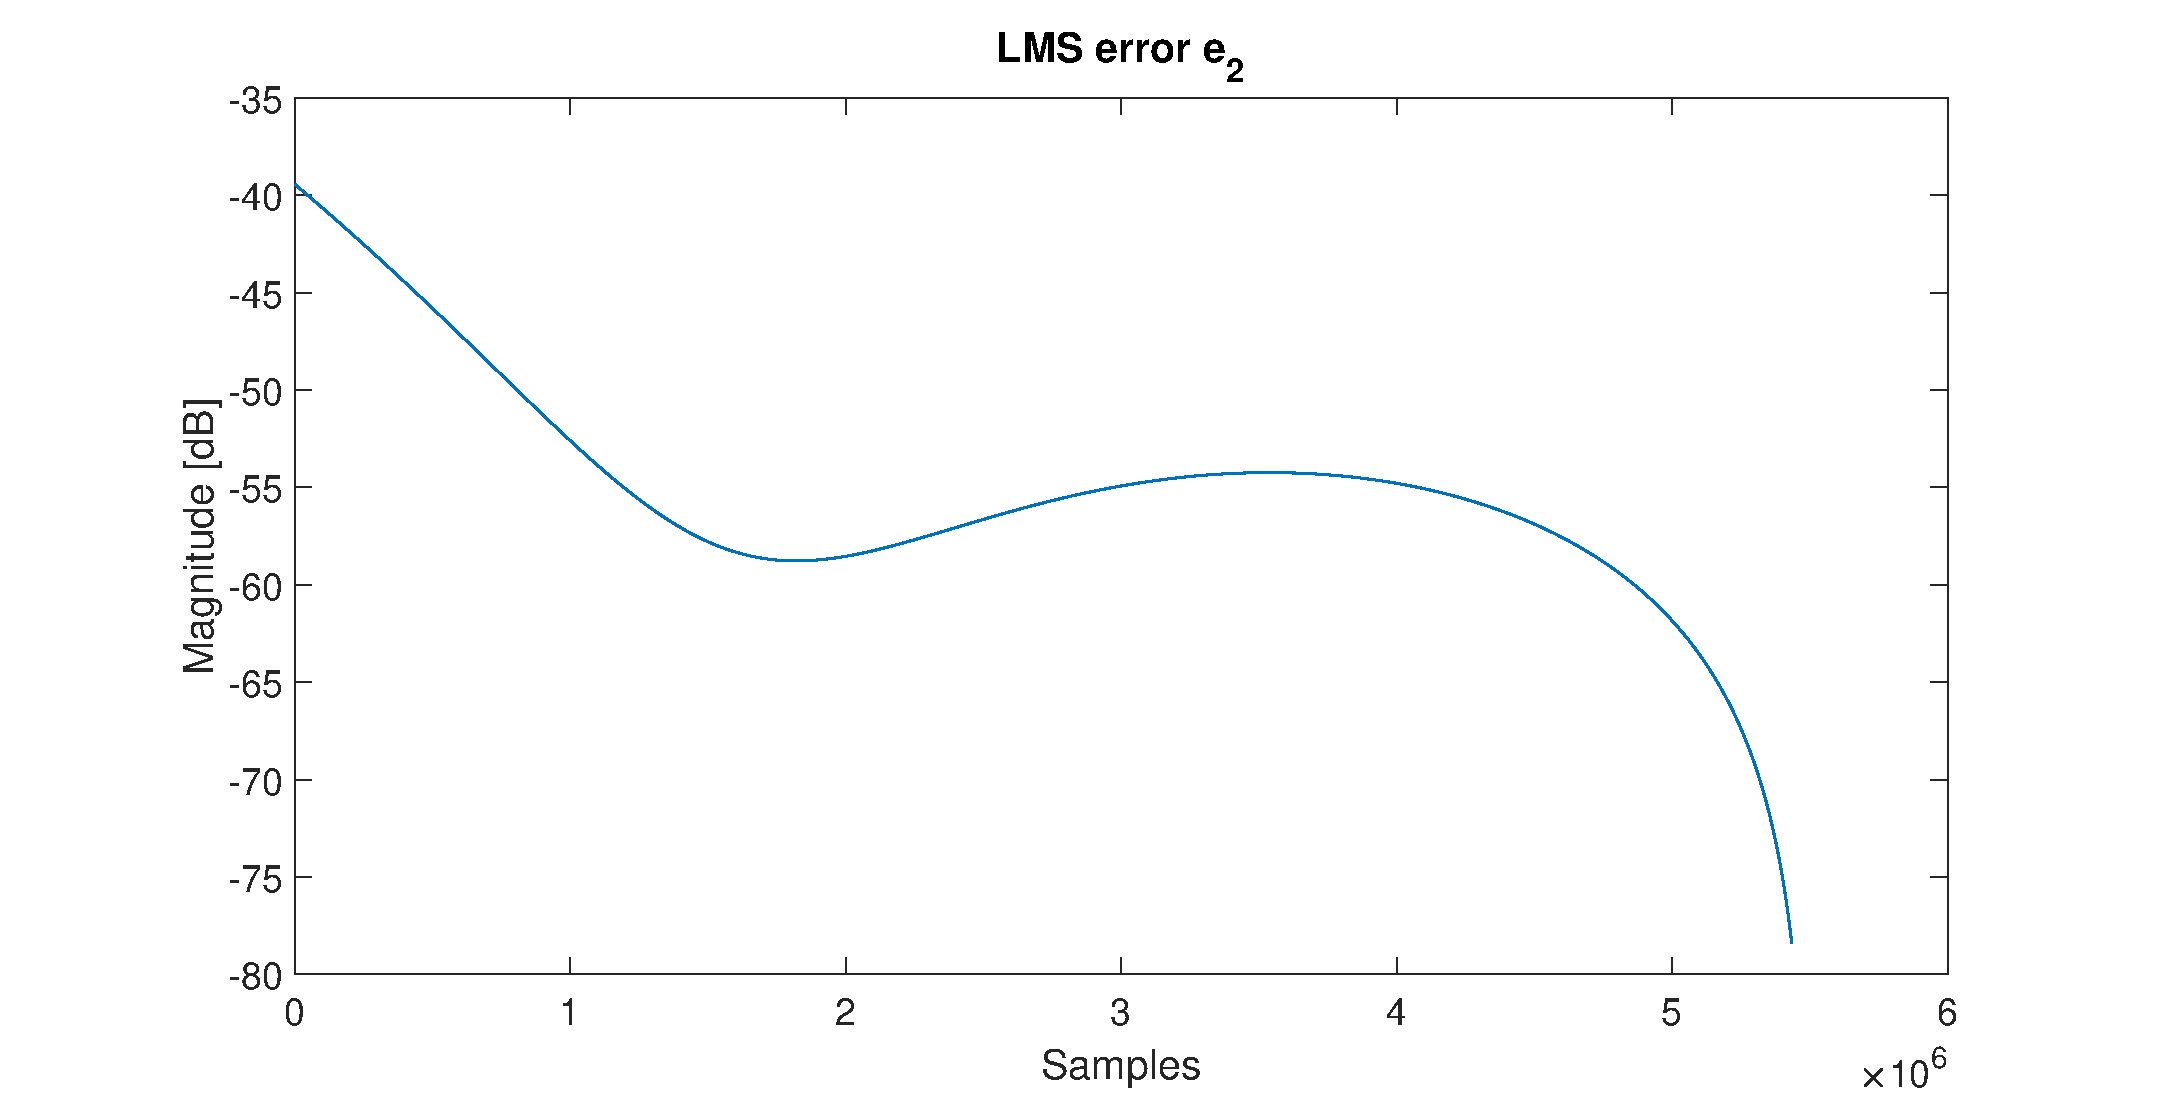
\includegraphics[width=1\textwidth]{Immagini/mse_e2}
		\caption{}
		\label{mse_e2}
	\end{subfigure}
	\caption{Confronto dell'MSE del canale (a) sinistro e (b) destro dell'algoritmo LMS.}
	\label{fig:mse_LMS}
\end{figure}
\end{frame}

\begin{frame}
\begin{figure}[h]
	\centering
	\begin{subfigure}{.45\textwidth}
		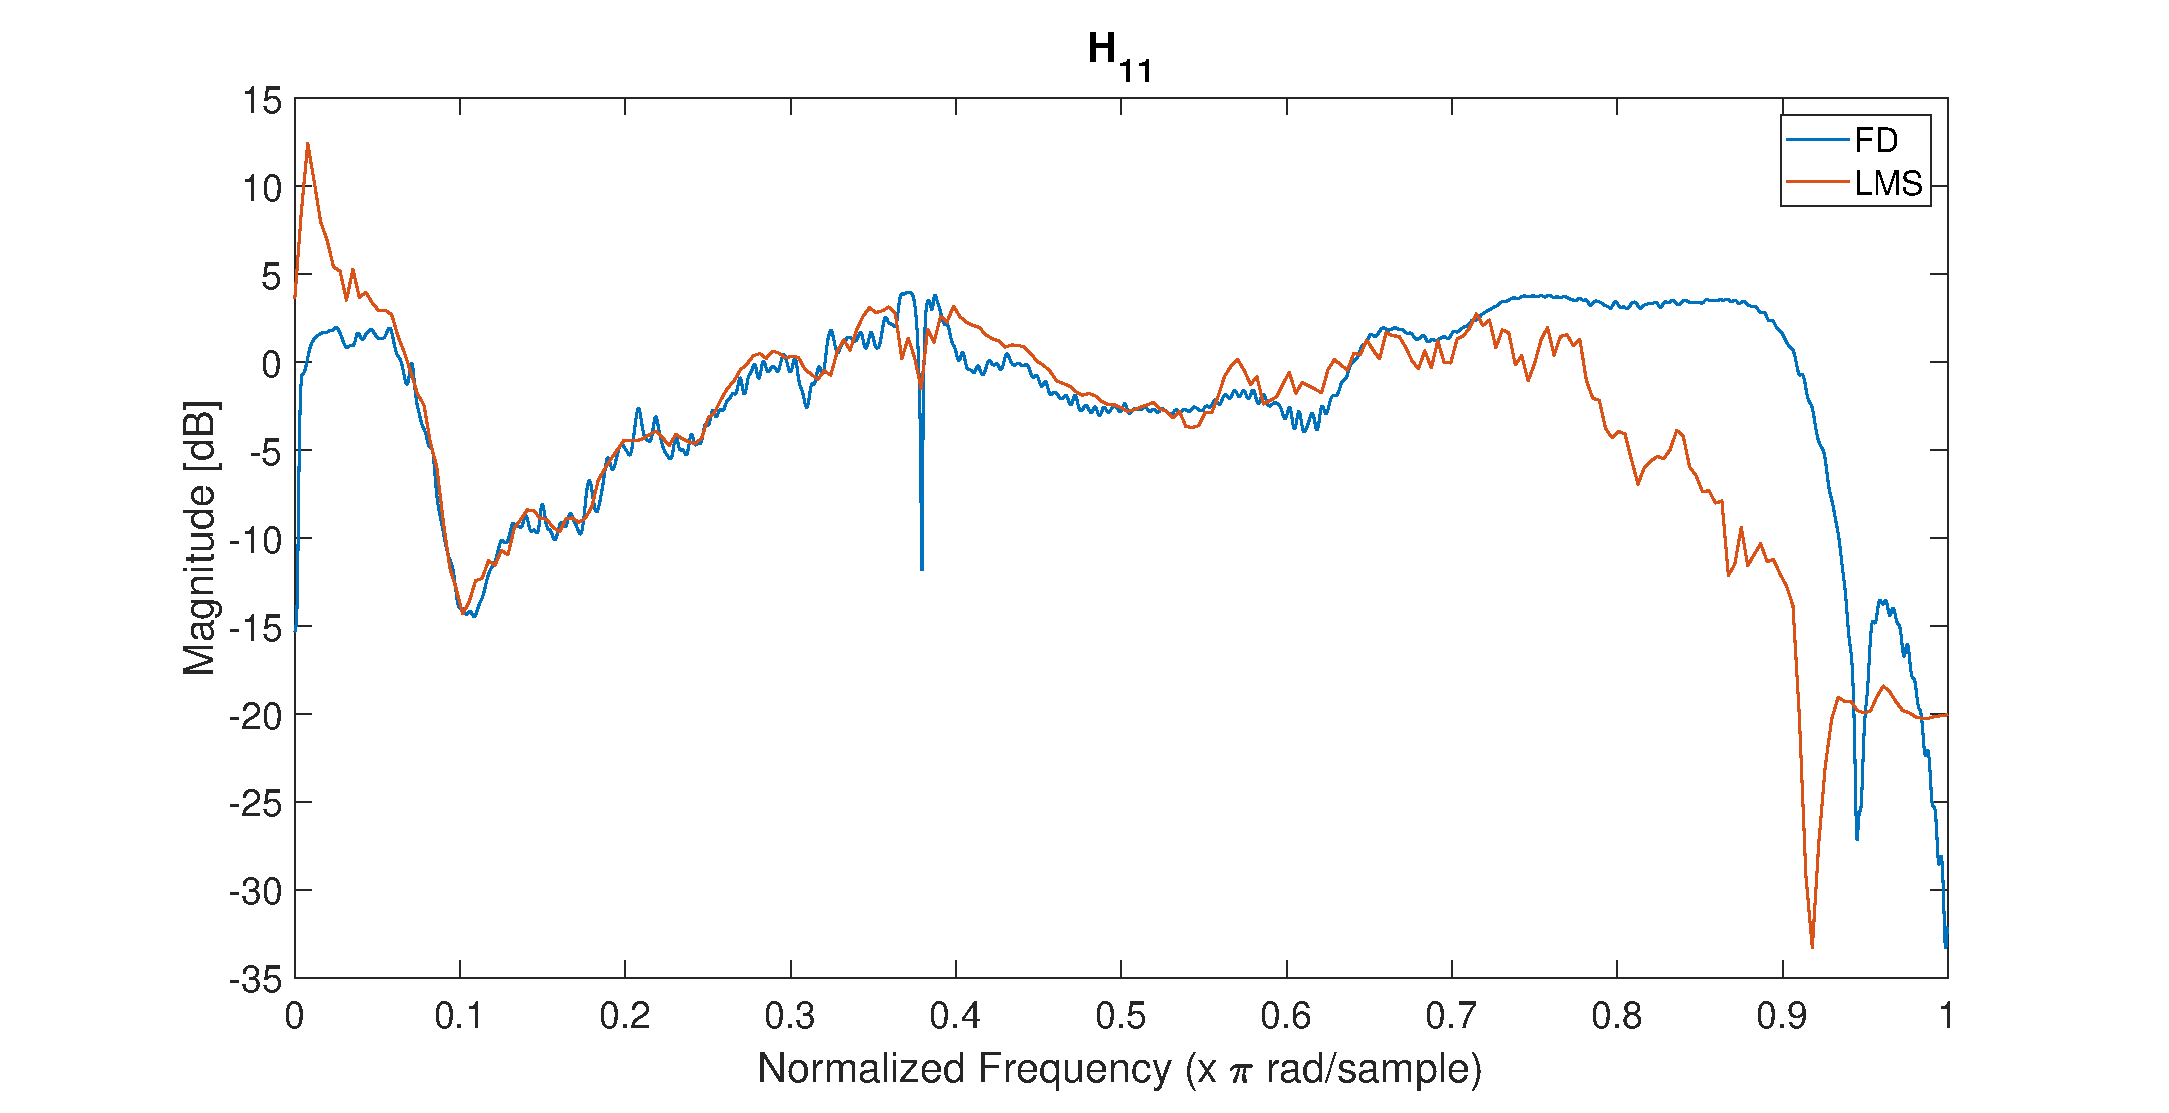
\includegraphics[width=1\textwidth]{Immagini/H11_FD_LMS}
		\caption{}
		\label{fig:Confronto_H11_LMS_FD}
	\end{subfigure}
	\hfill
	\begin{subfigure}{.45\textwidth}
		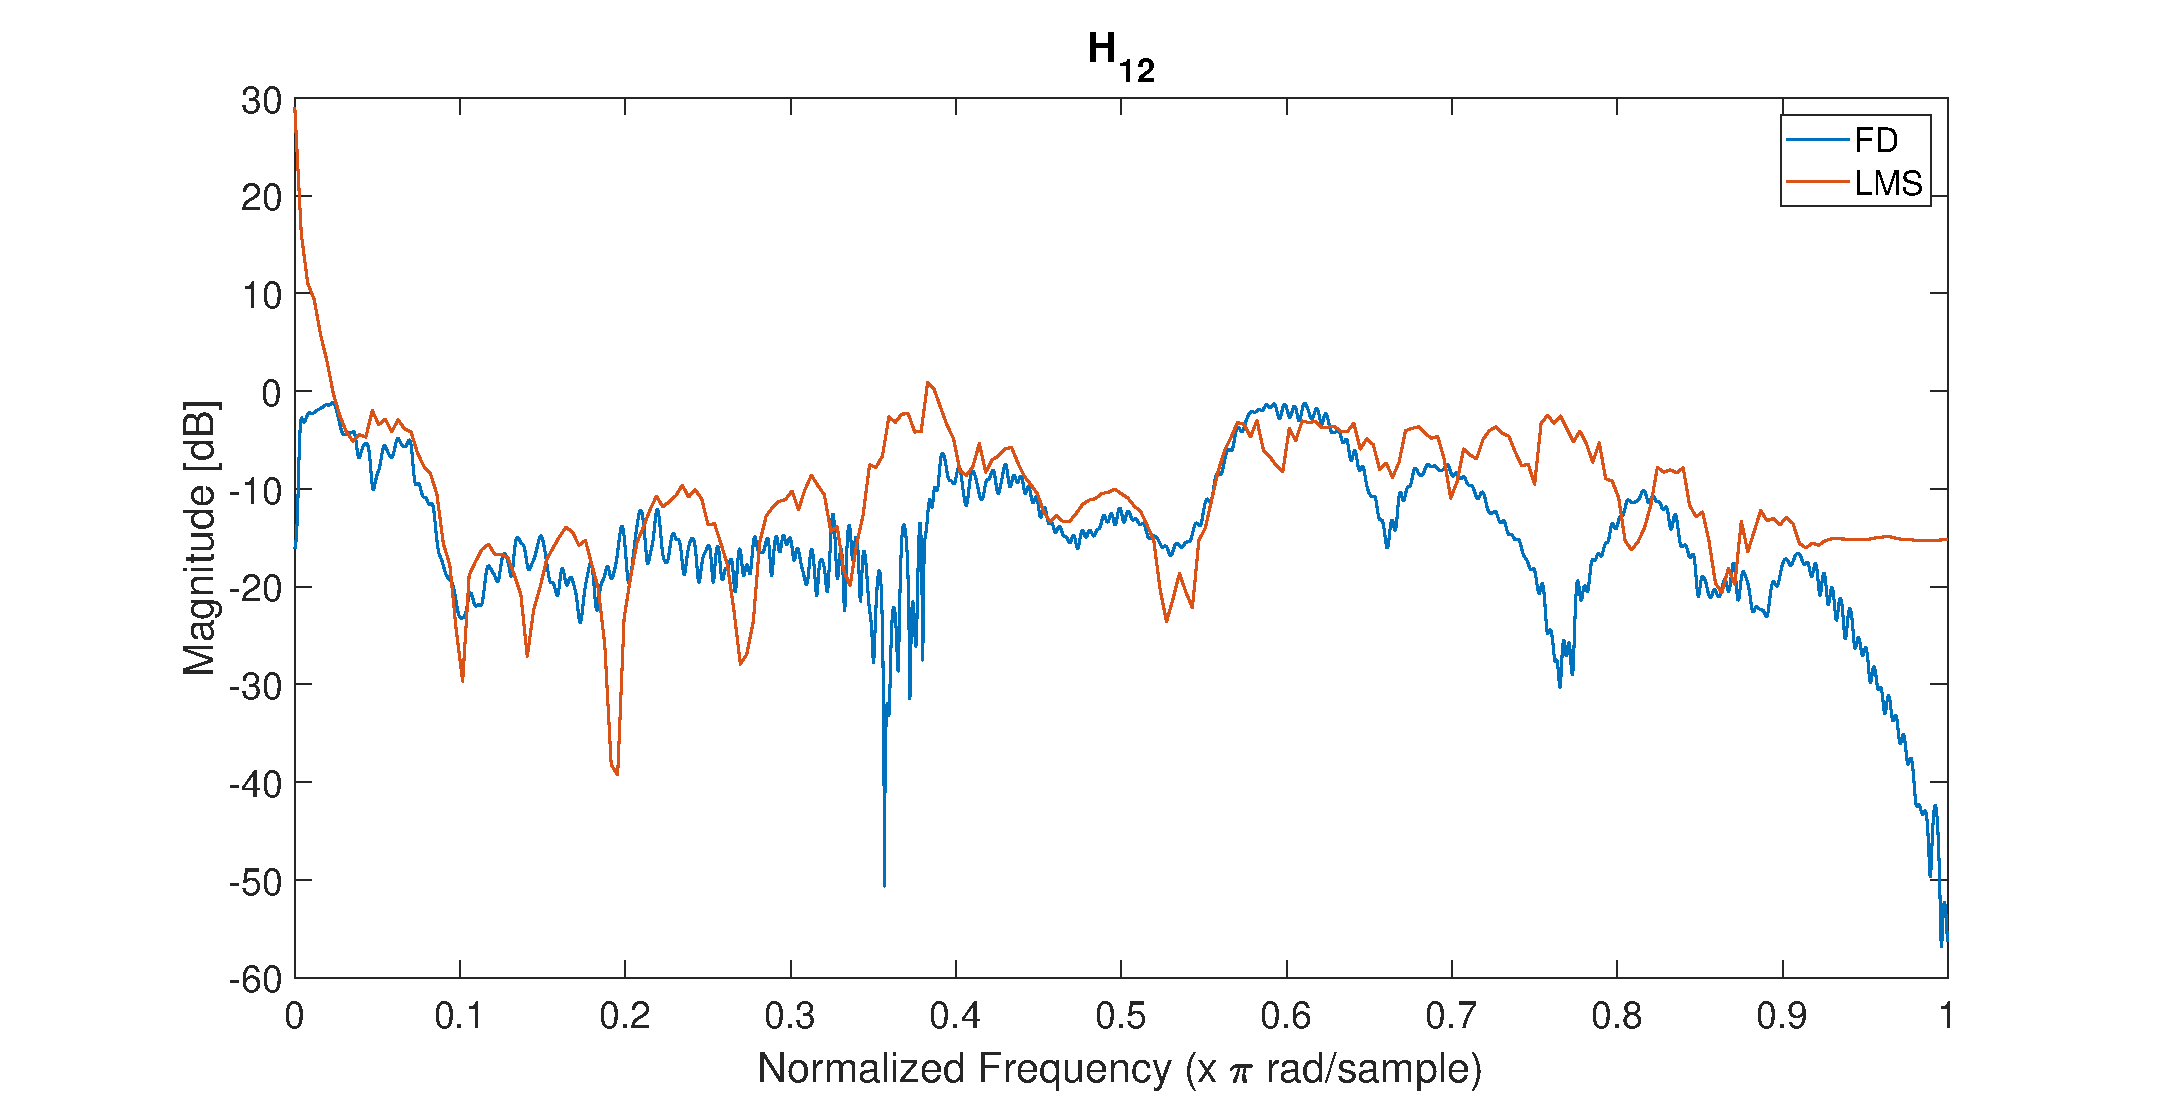
\includegraphics[width=1\textwidth]{Immagini/H12_FD_LMS}
		\caption{}
		\label{fig:Confronto_H12_LMS_FD}
	\end{subfigure}
	\vfill
	\begin{subfigure}{.45\textwidth}
		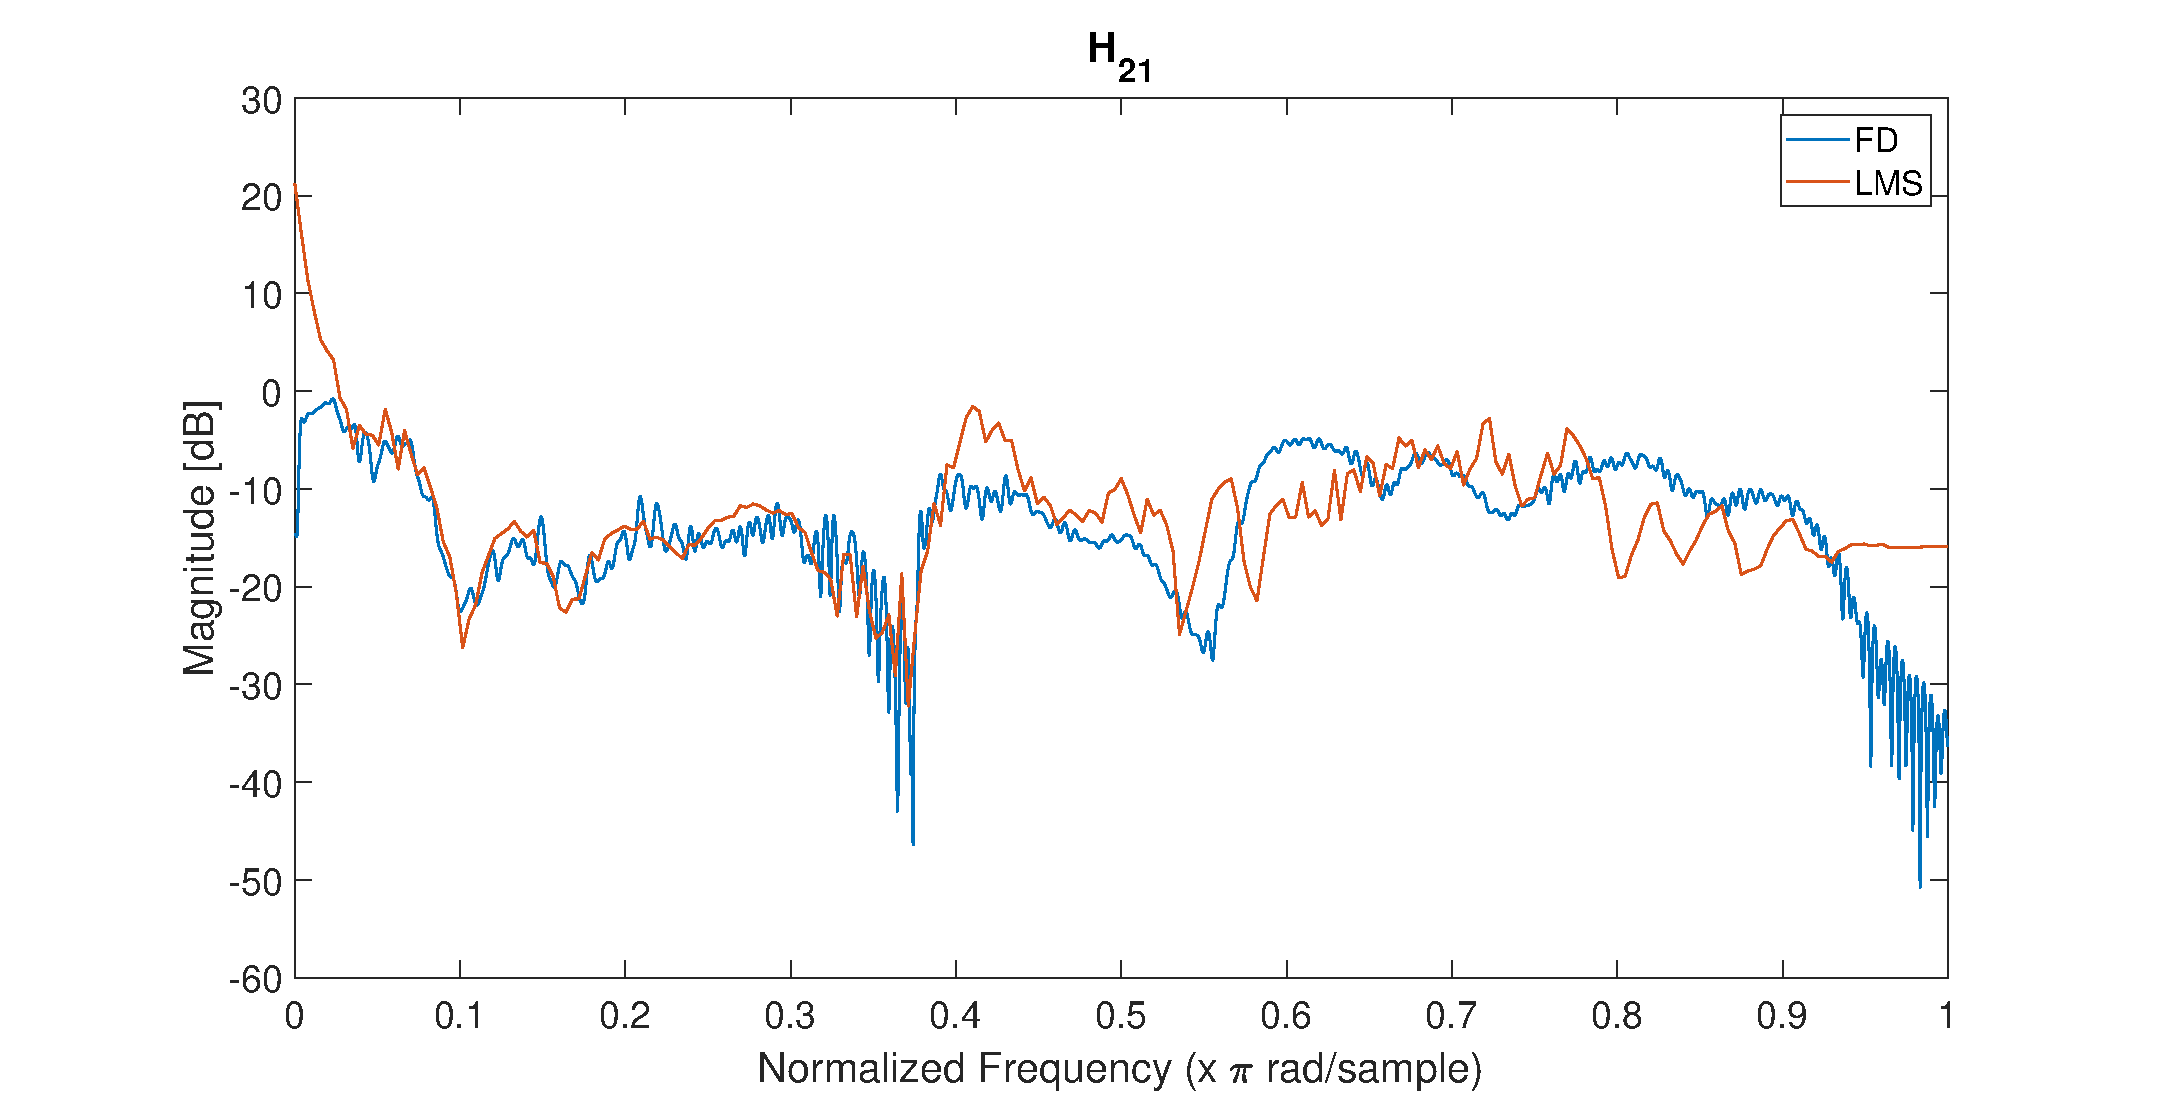
\includegraphics[width=1\textwidth]{Immagini/H21_FD_LMS}
		\caption{}
		\label{fig:Confronto_H21_LMS_FD}
	\end{subfigure}
	\hfill
	\begin{subfigure}{.45\textwidth}
		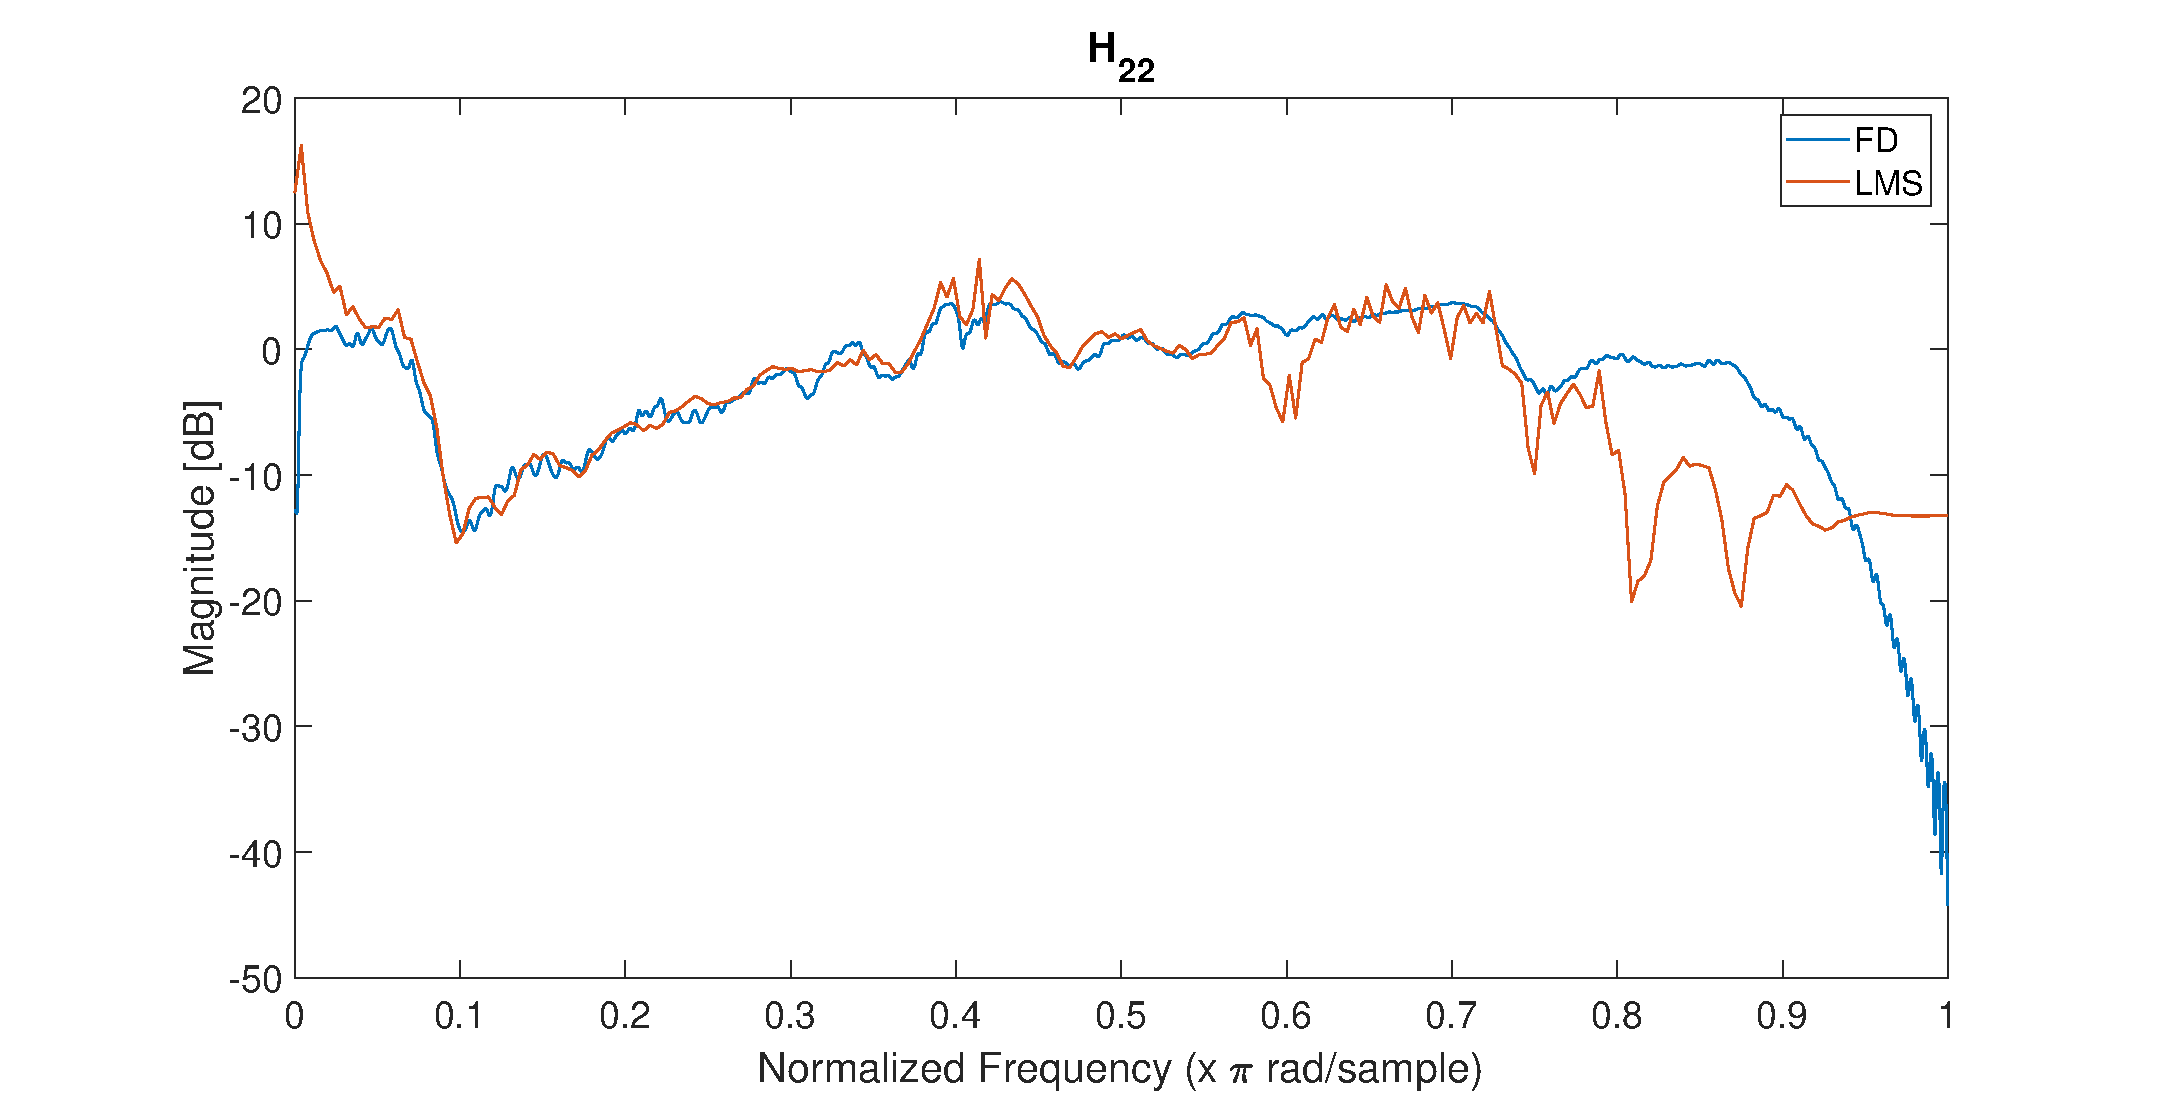
\includegraphics[width=1\textwidth]{Immagini/H22_FD_LMS}
		\caption{}
		\label{fig:Confronto_H22_LMS_FD}
	\end{subfigure}
	\caption{Confronto dei filtri di cancellazione del crosstalk (a) $H_{11}$, (b) $H_{12}$, (c) $H_{21}$, (d) $H_{22}$ di LMS e Fast Deconvolution.}
	\label{fig:confronto_H_LMS_FD}
\end{figure}
\end{frame}

\begin{frame}
\begin{figure}[h]
	\centering
	\begin{subfigure}{.45\textwidth}
		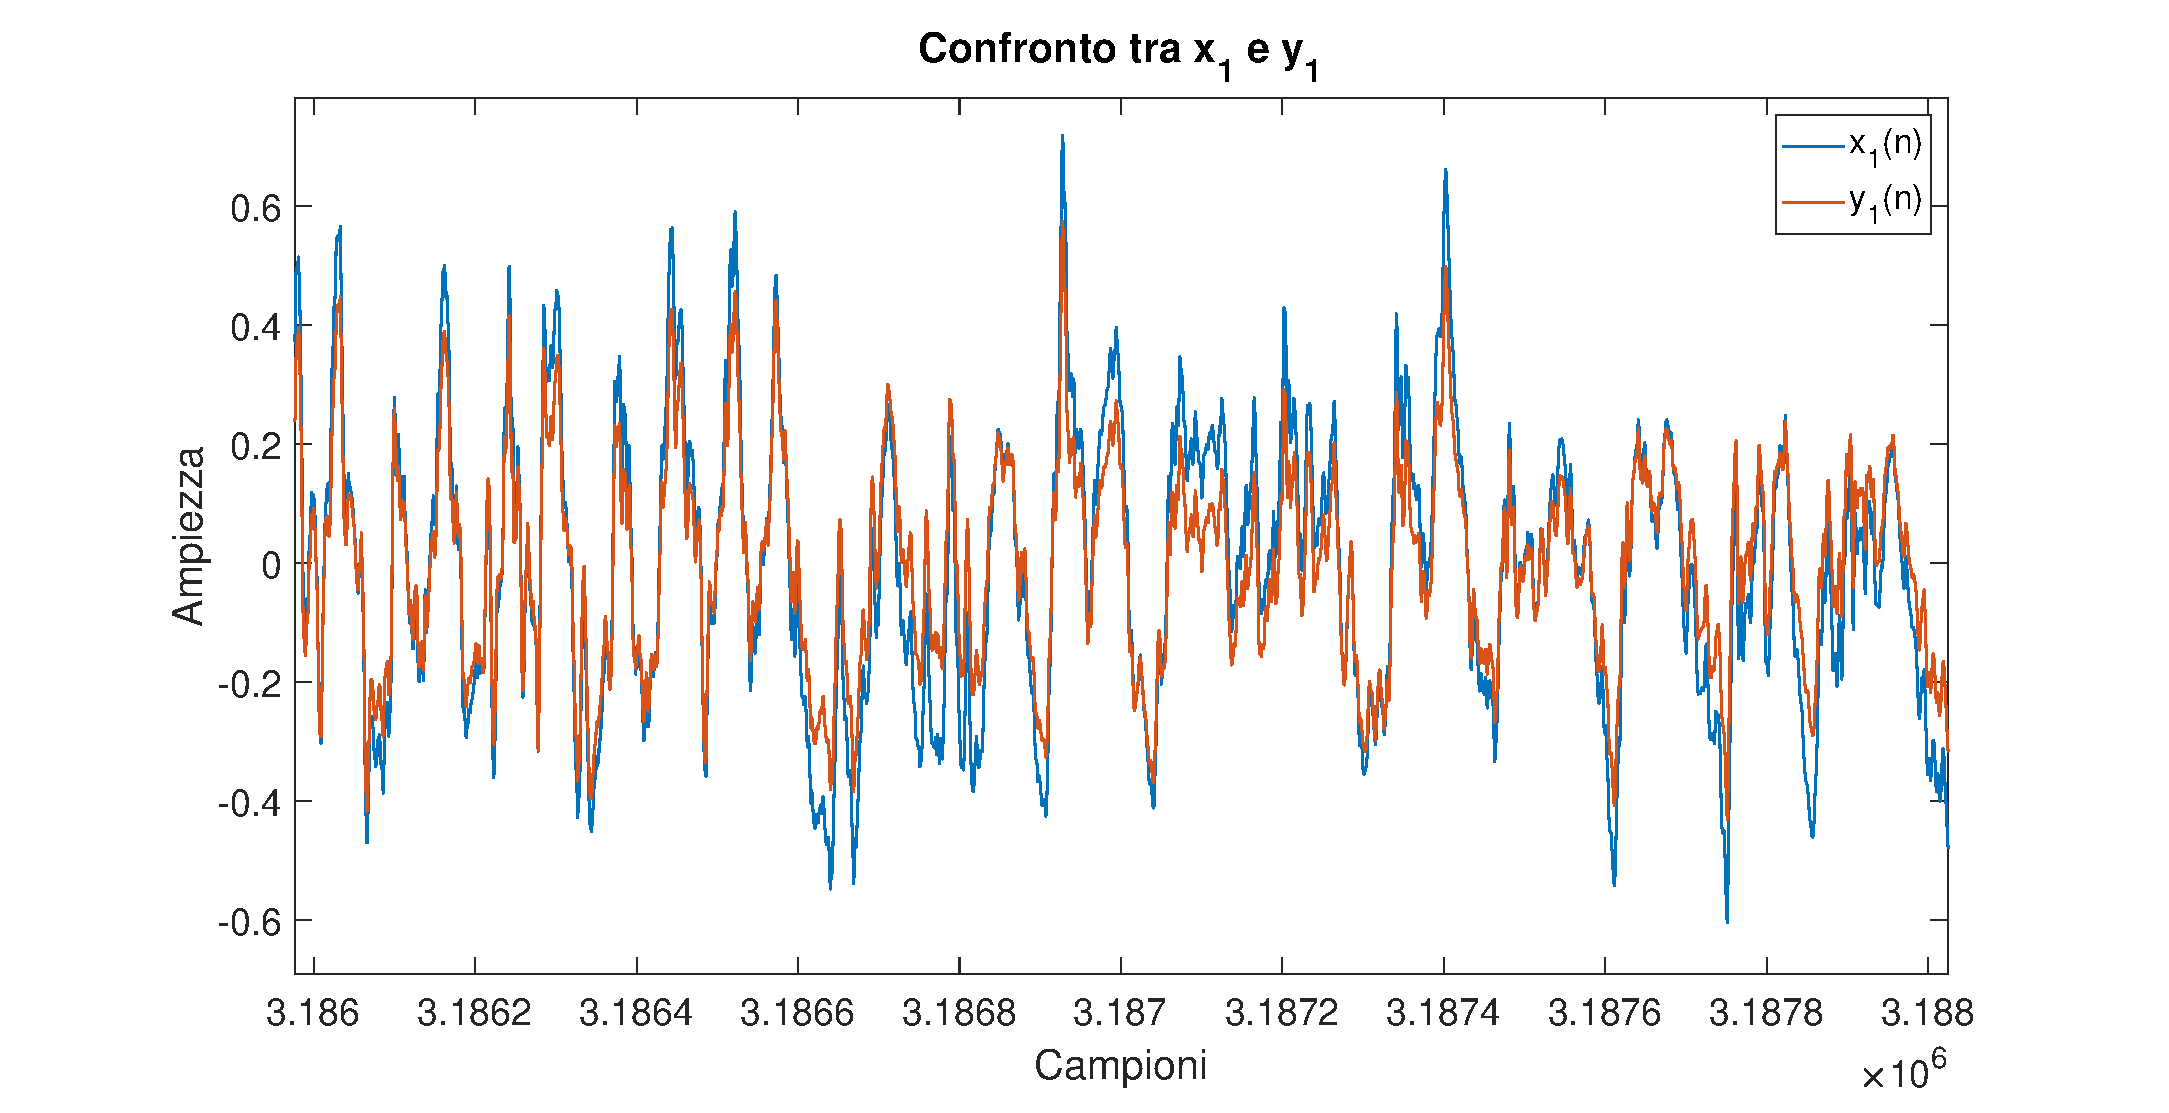
\includegraphics[width=1\textwidth]{Immagini/x1_y1_FD}
		\caption{}
		\label{fig:x1_y1_FD}
	\end{subfigure}
	\hfill
	\begin{subfigure}{.45\textwidth}
		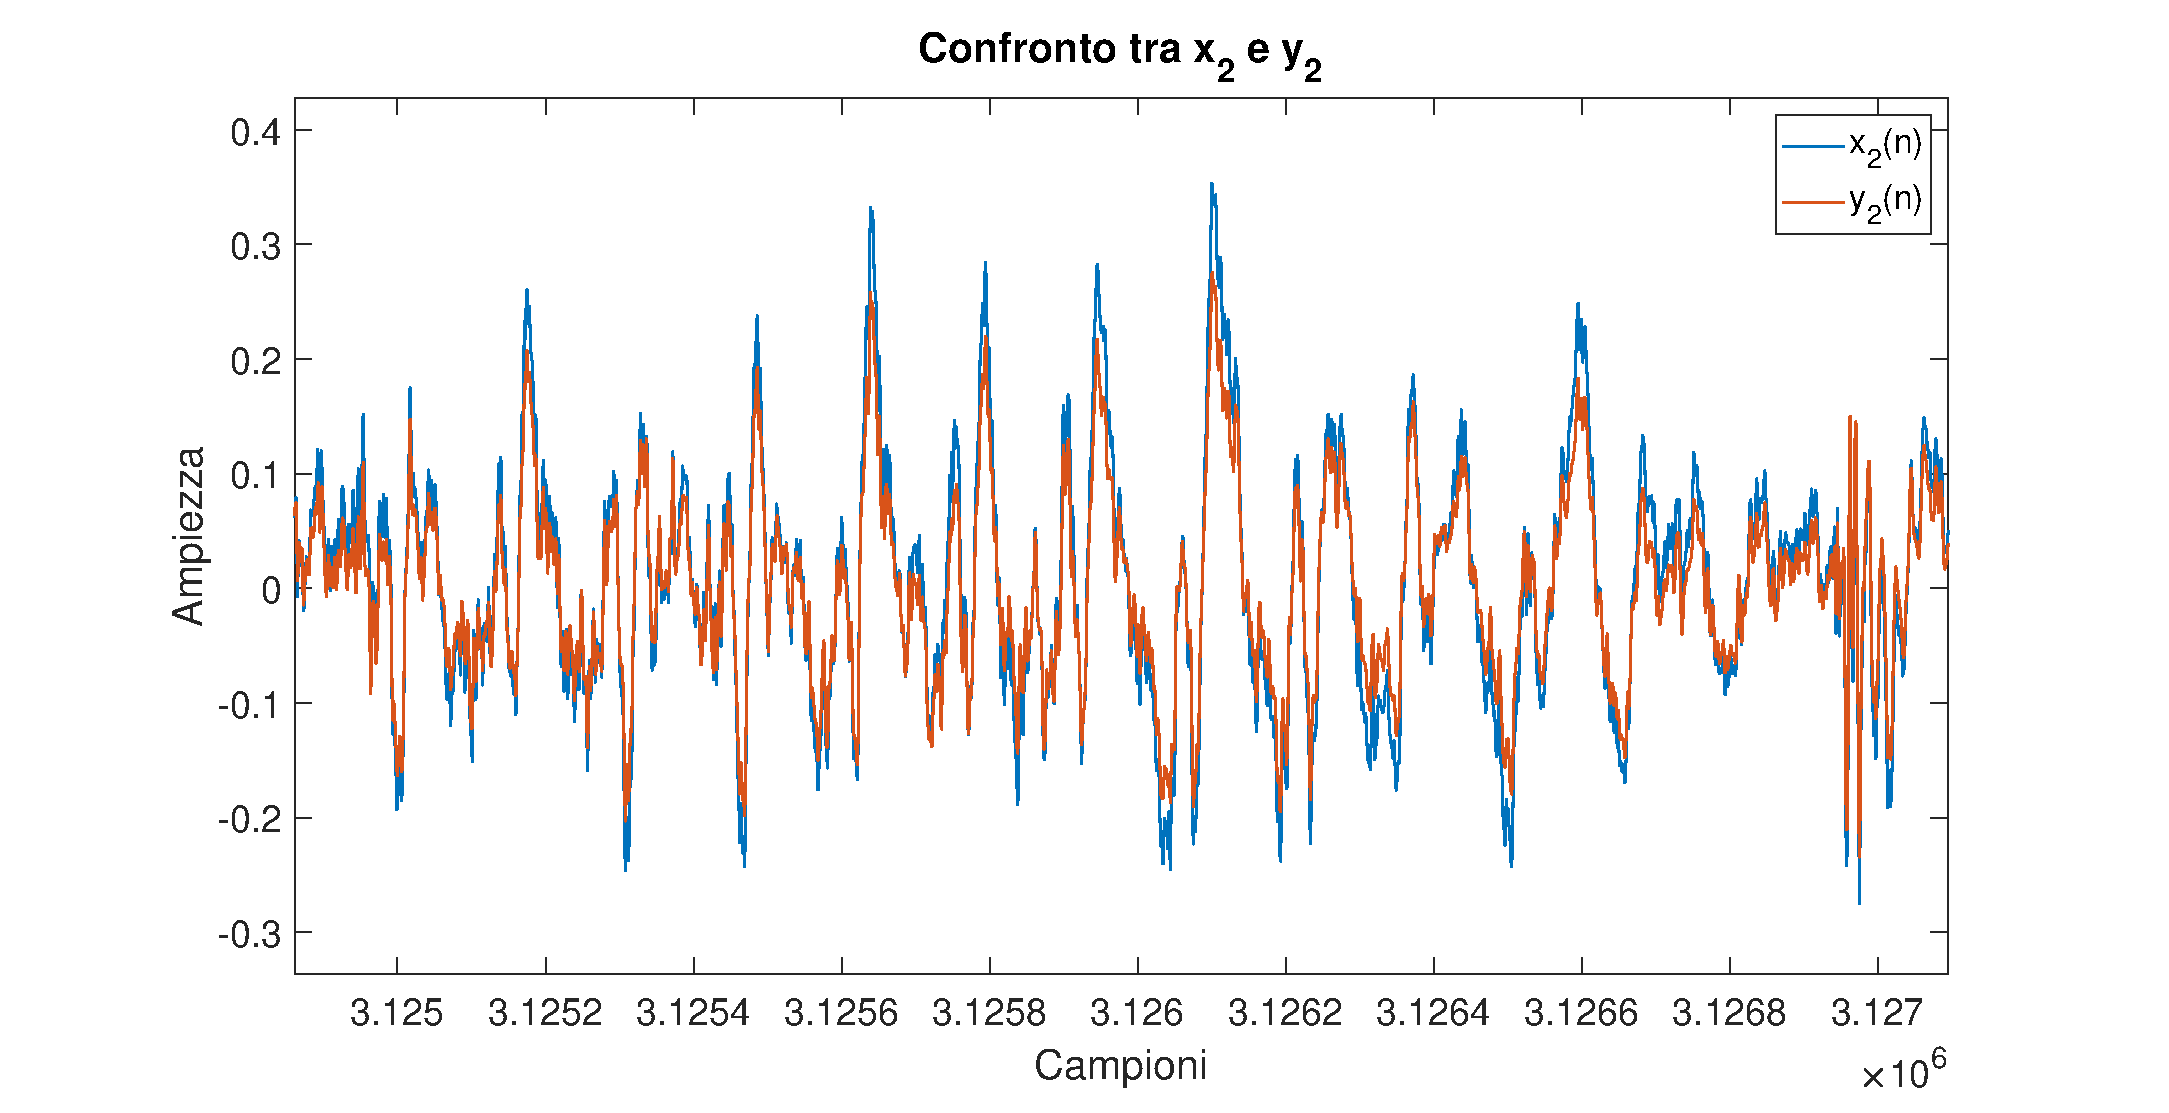
\includegraphics[width=1\textwidth]{Immagini/x2_y2_FD}
		\caption{}
		\label{fig:x2_y2_FD}
	\end{subfigure}
	\vfill
	\begin{subfigure}{.45\textwidth}
		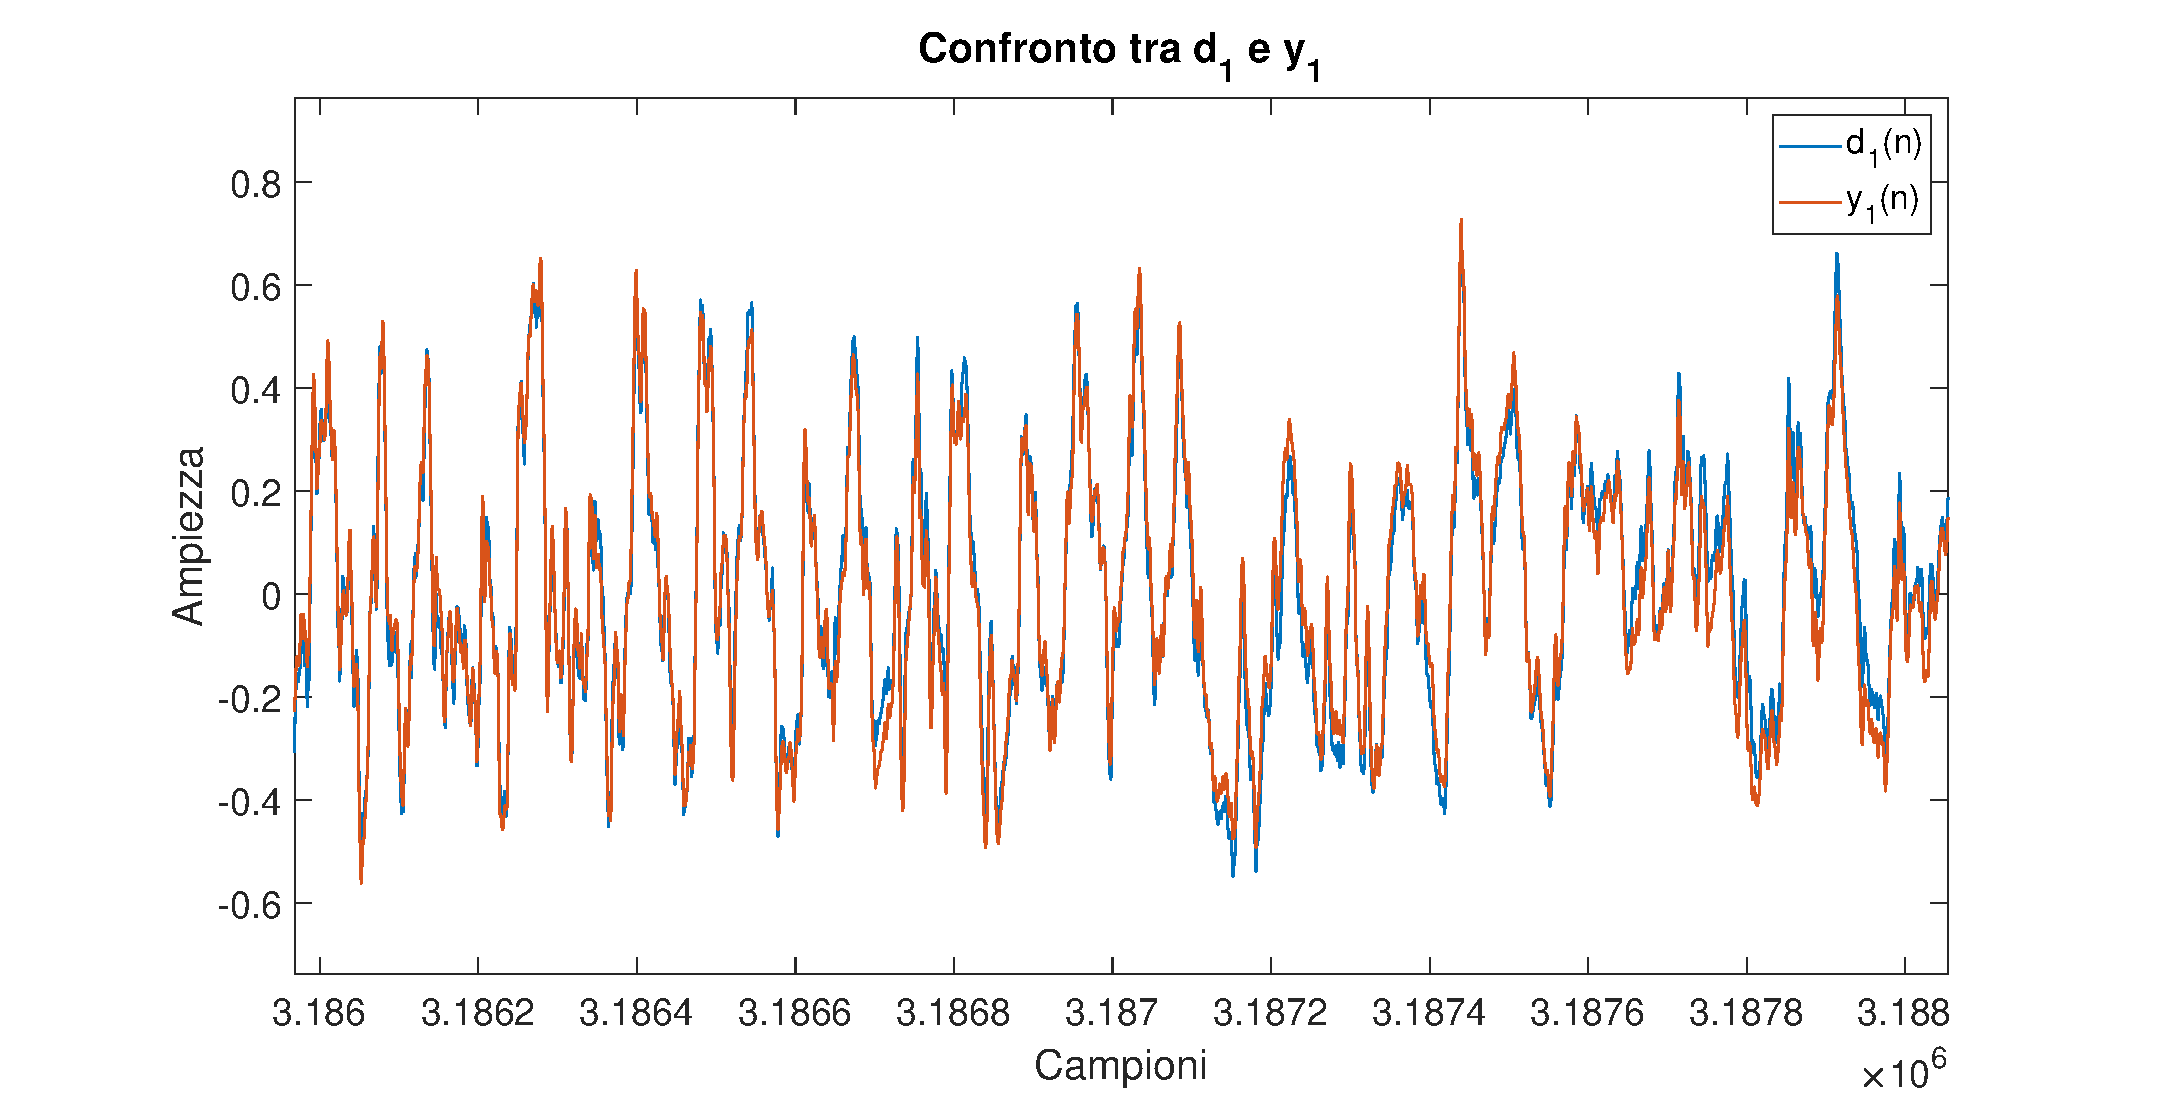
\includegraphics[width=1\textwidth]{Immagini/d1_y1_LMS}
		\caption{}
		\label{fig:d1_y1_LMS}
	\end{subfigure}
	\hfill
	\begin{subfigure}{.45\textwidth}
		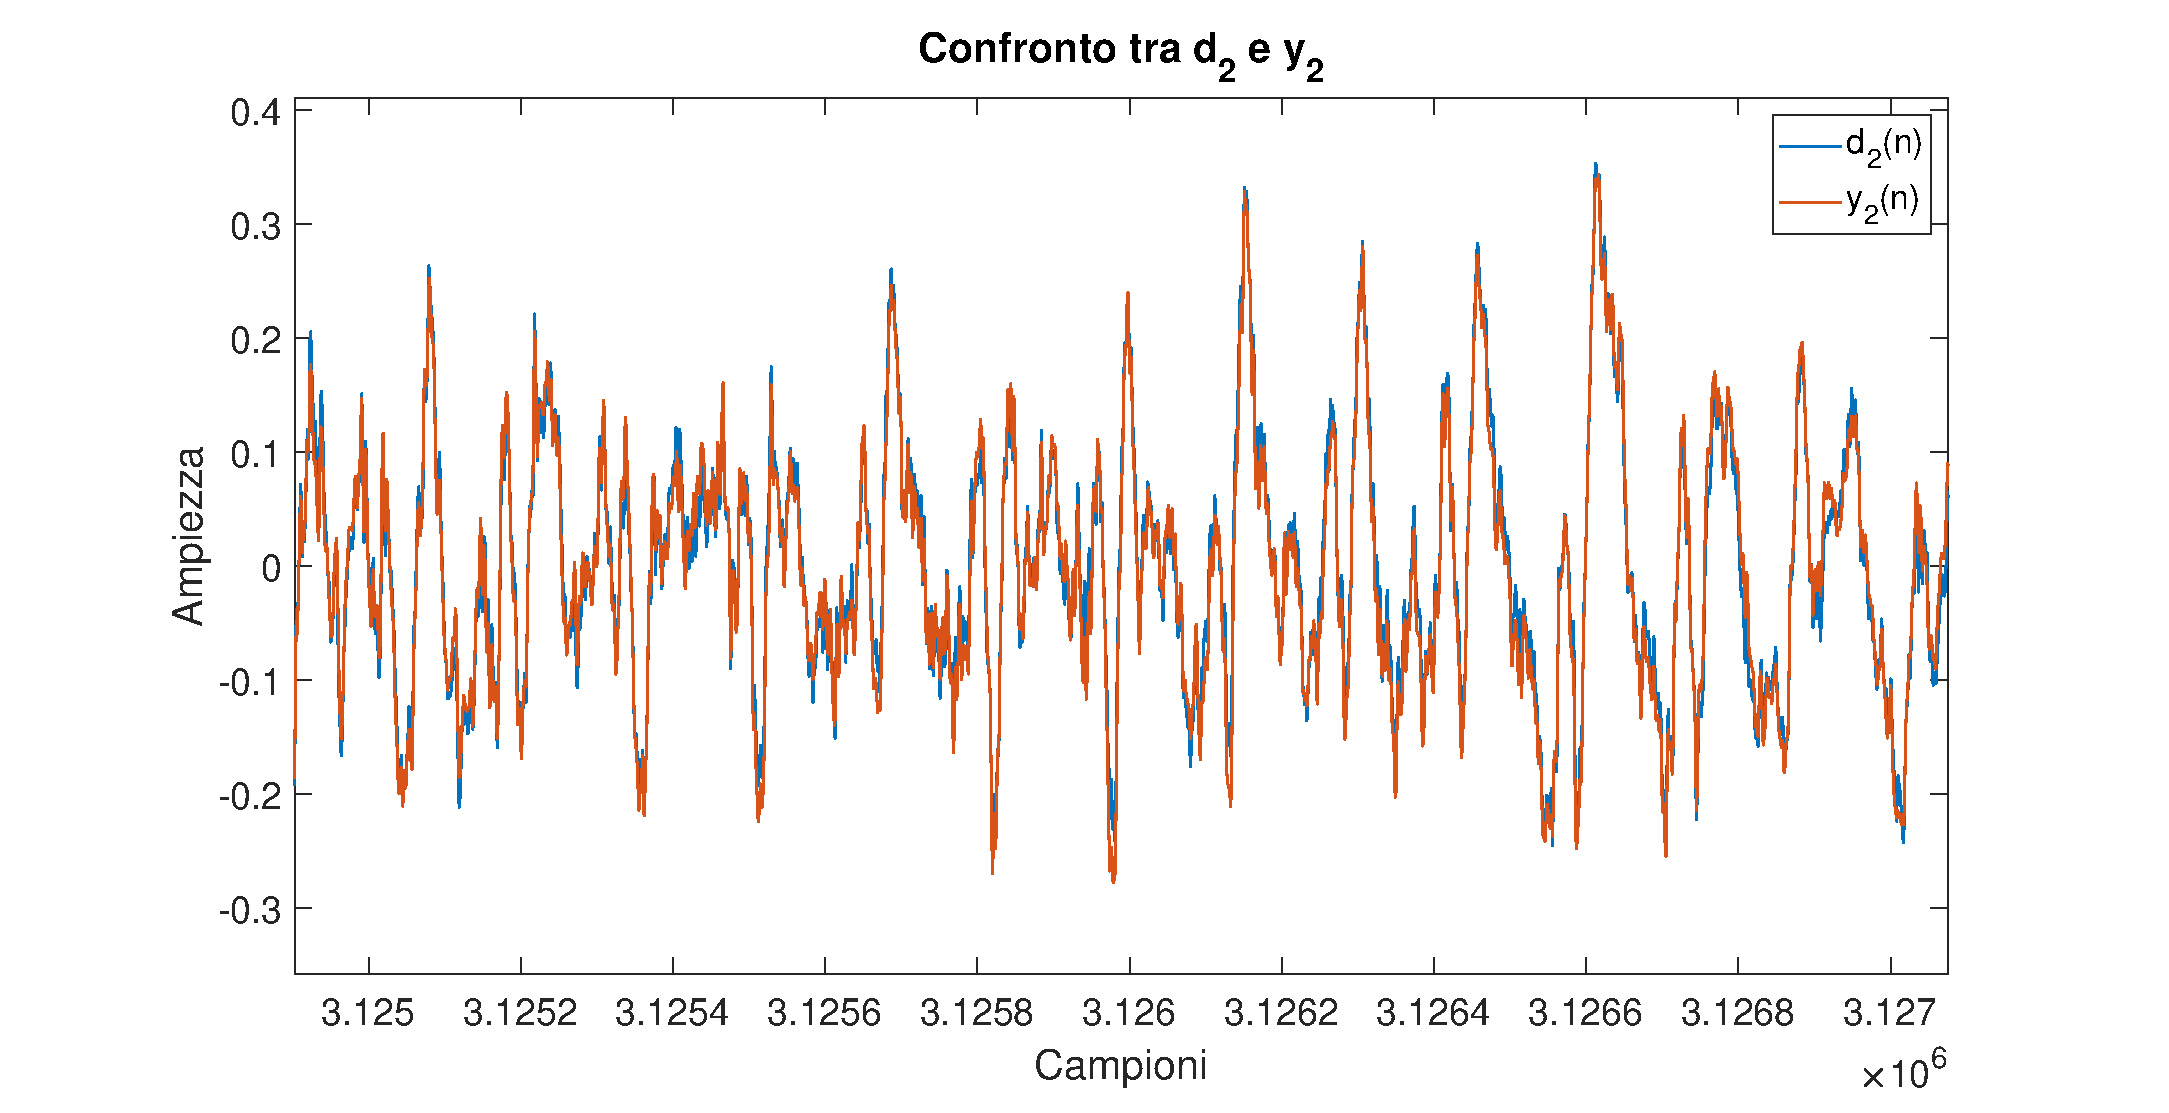
\includegraphics[width=1\textwidth]{Immagini/d2_y2_LMS}
		\caption{}
		\label{fig:d2_y2_LMS}
	\end{subfigure}
	\caption{Confronto degli ingressi e le uscite (a) sinistro e (b) destro della Fast Deconvolution, (c) sinistro e (d) destro di LMS.}
	\label{fig:confronto_ingressi_uscite_LMS_FD}
\end{figure}
\end{frame}

\begin{frame}{Risultati NU-Tech}
\begin{figure}[h]
	\centering
	\begin{subfigure}{.45\textwidth}
		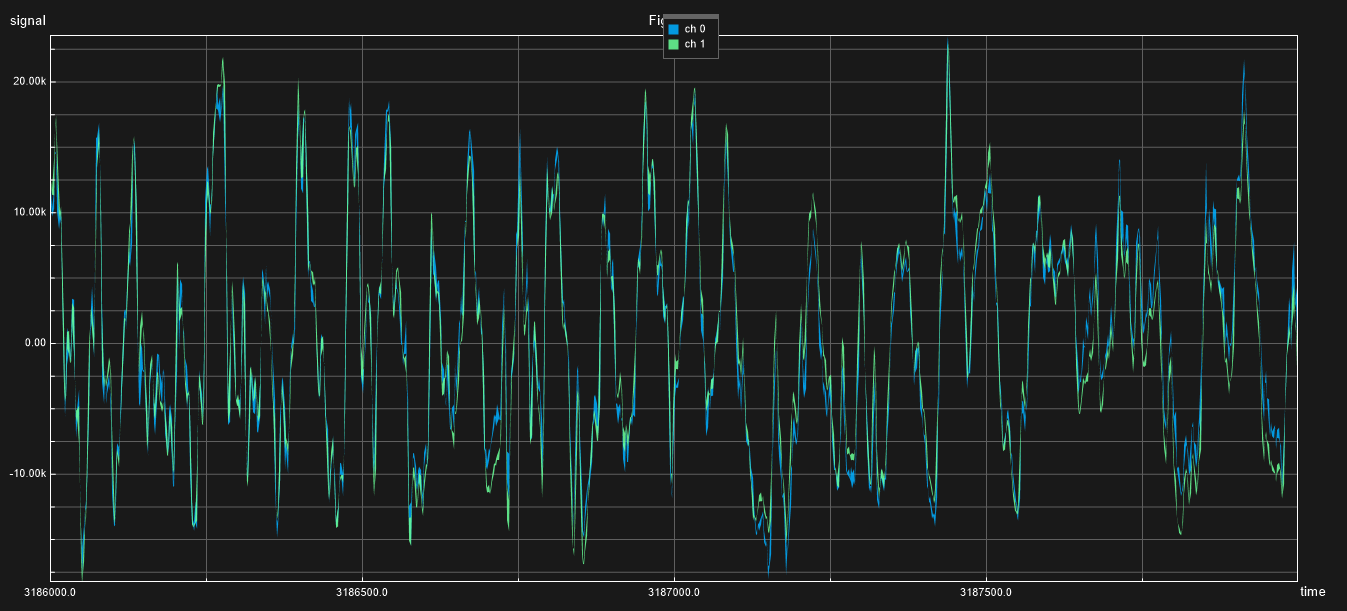
\includegraphics[width=1\textwidth]{Immagini/x1_y1_FD_nutech}
		\caption{}
		\label{fig:x1_y1_FD_nutech}
	\end{subfigure}
	\hfill
	\begin{subfigure}{.45\textwidth}
			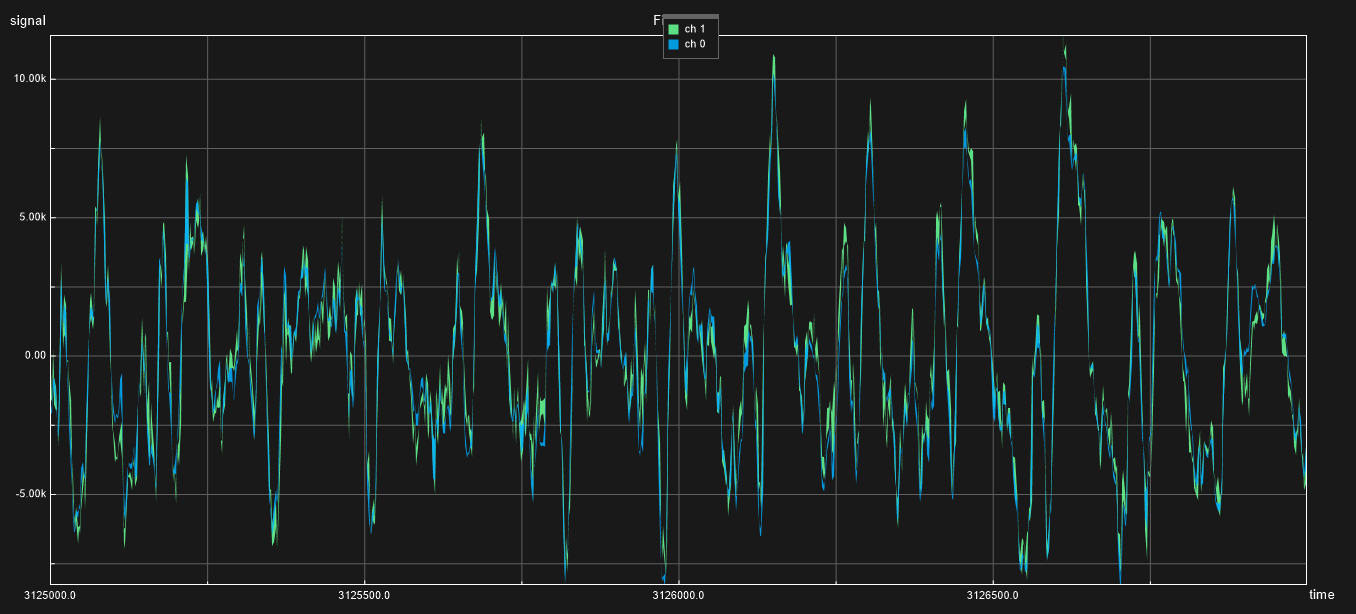
\includegraphics[width=1\textwidth]{Immagini/x2_y2_FD_nutech}
			\caption{}
			\label{fig:x2_y2_FD_nutech}
	\end{subfigure}
	\vfill
	\begin{subfigure}{.45\textwidth}
		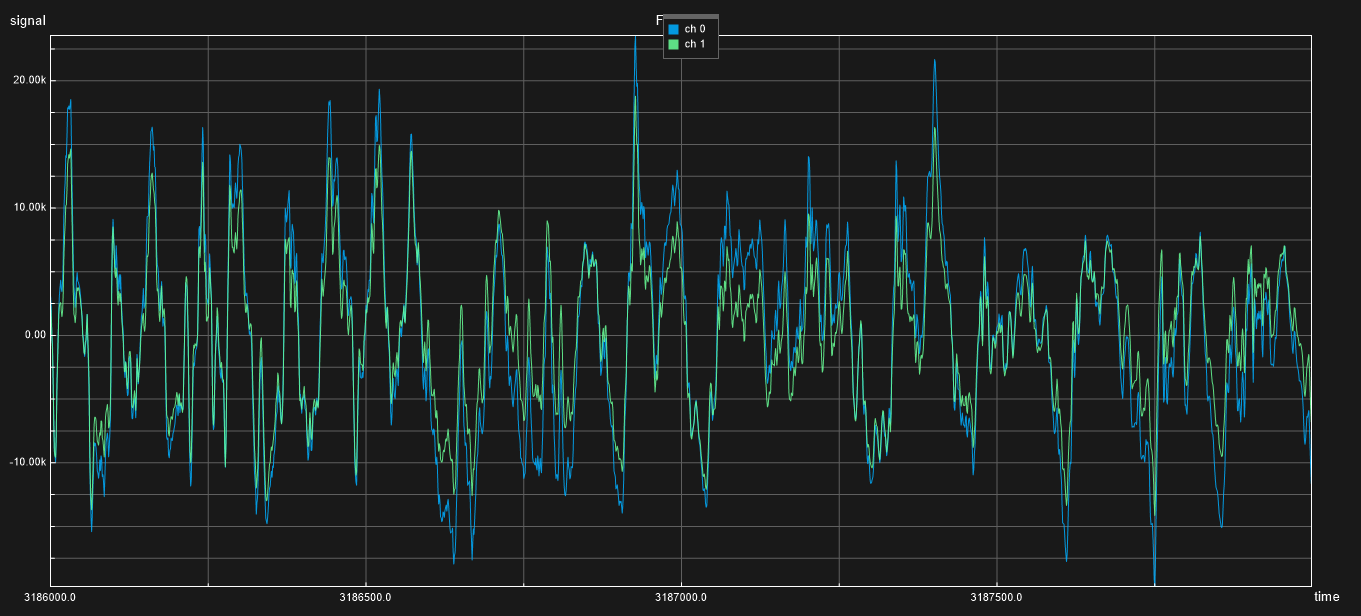
\includegraphics[width=1\textwidth]{Immagini/d1_y1_LMS_nutech}
		\caption{}
		\label{fig:d1_y1_LMS_nutech}
	\end{subfigure}
	\hfill
	\begin{subfigure}{.45\textwidth}
		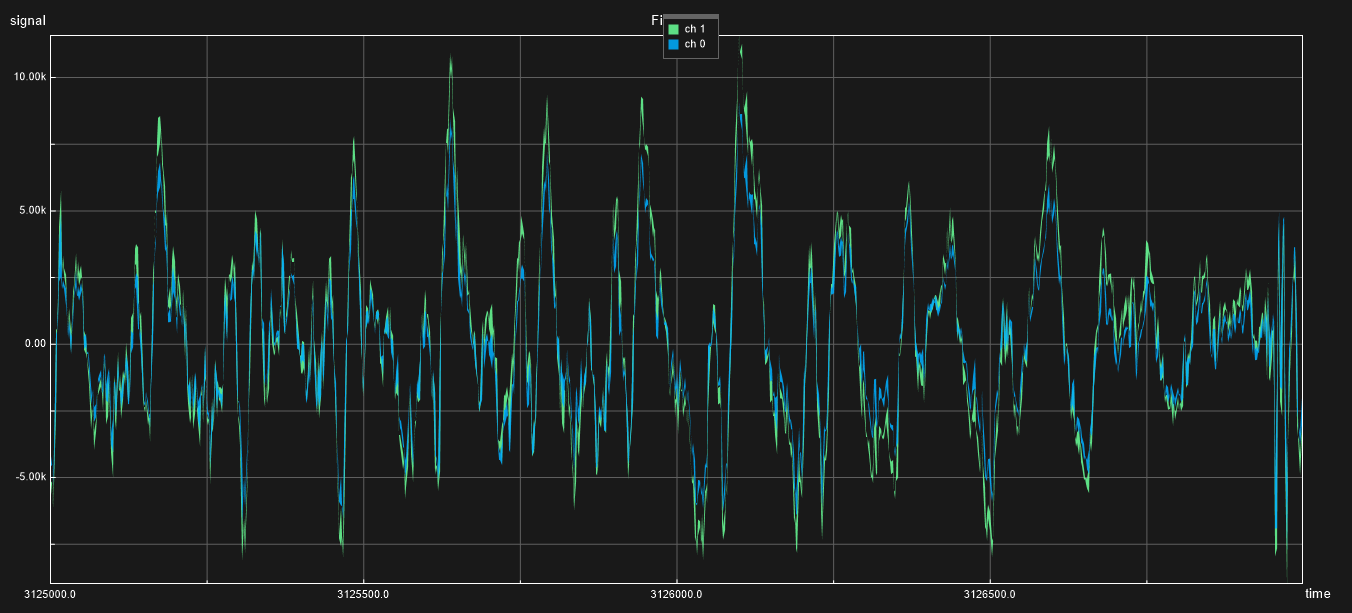
\includegraphics[width=1\textwidth]{Immagini/d2_y2_LMS_nutech}
		\caption{}
		\label{fig:d2_y2_LMS_nutech}
	\end{subfigure}
		\caption{Confronto degli ingressi e le uscite (a) sinistro e (b) destro della Fast Deconvolution, (c) sinistro e (d) destro di LMS.}
		\label{fig:confronto_ingressi_uscita_LMS_nutech}
\end{figure}
\end{frame}

\begin{frame}
\begin{figure}[h]
	\centering
	\begin{subfigure}{.45\textwidth}
		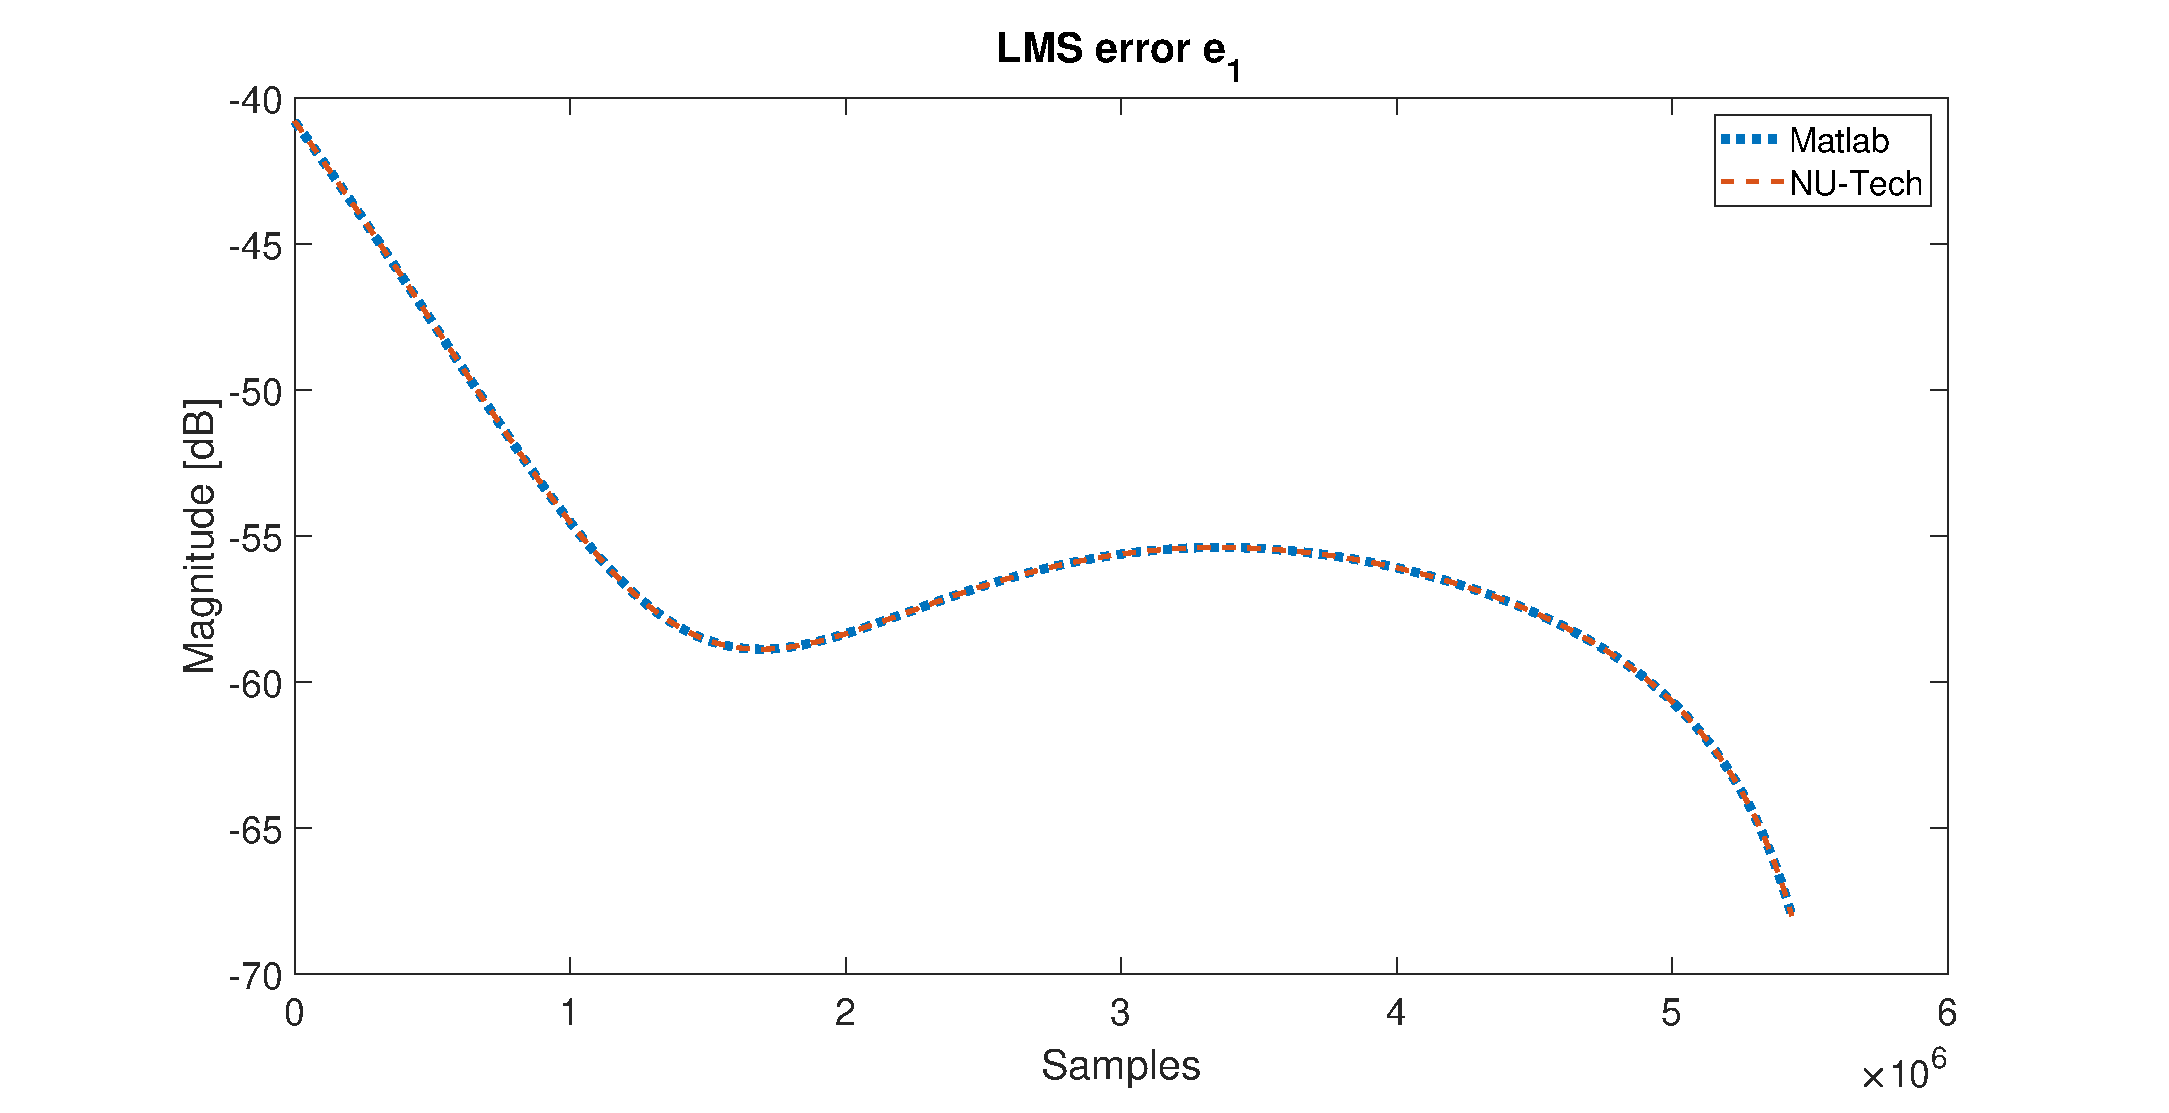
\includegraphics[width=1\textwidth]{Immagini/mse_e1_matlab_nutech}
		\caption{}
		\label{fig:mse_e1_matlab_nutech}
	\end{subfigure}
	\vfill
	\begin{subfigure}{.45\textwidth}
			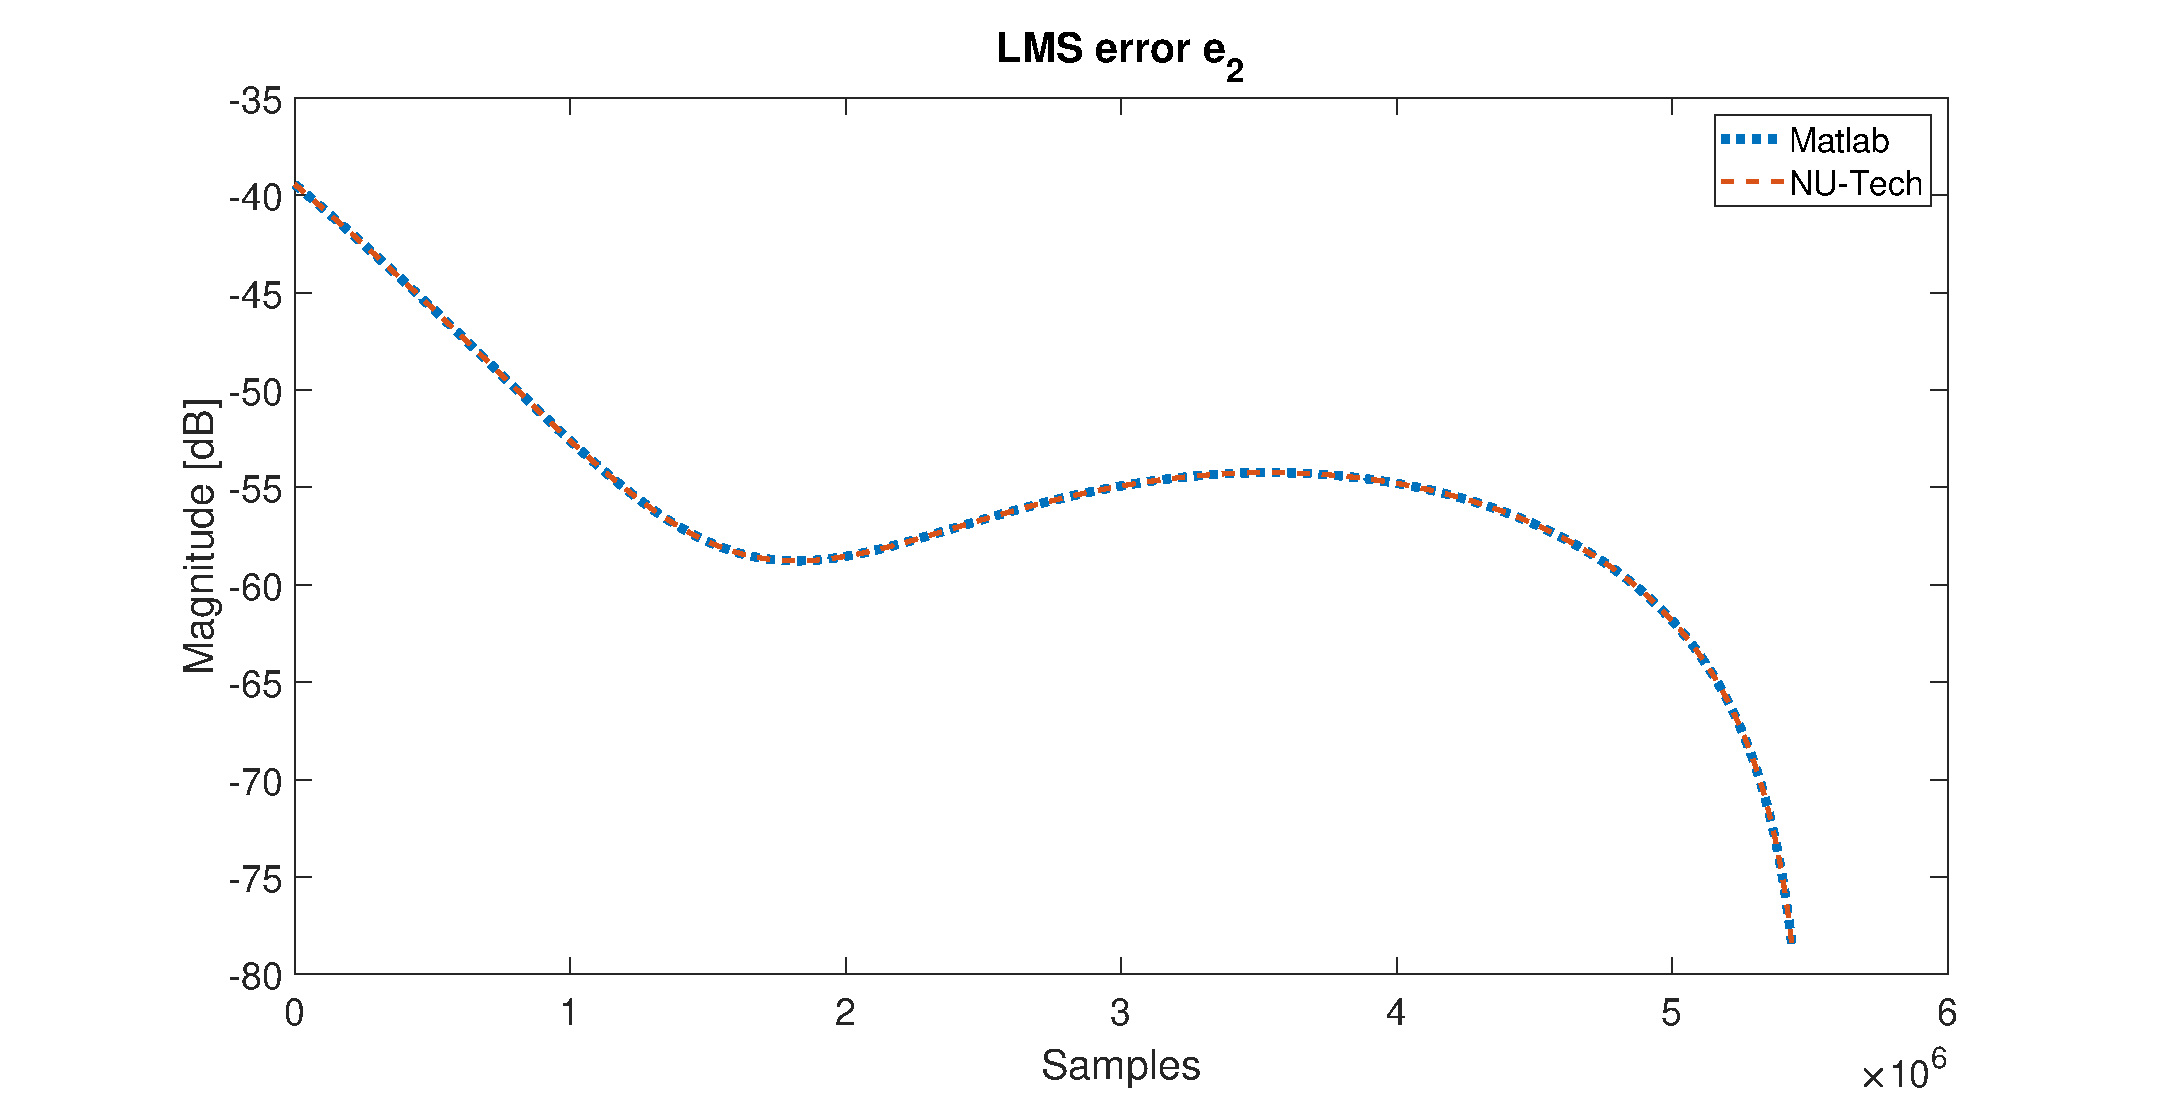
\includegraphics[width=1\textwidth]{Immagini/mse_e2_matlab_nutech}
			\caption{}
			\label{fig:mse_e2_matlab_nutech}
	\end{subfigure}
	\caption{Confronto dell'MSE del canale (a) sinistro e (b) destro dell'algoritmo LMS.}
	\label{fig:mse_matlab_nutech}
\end{figure}
\end{frame}

\begin{frame}
\begin{figure}[h]
	\centering
	\begin{subfigure}{.45\textwidth}
		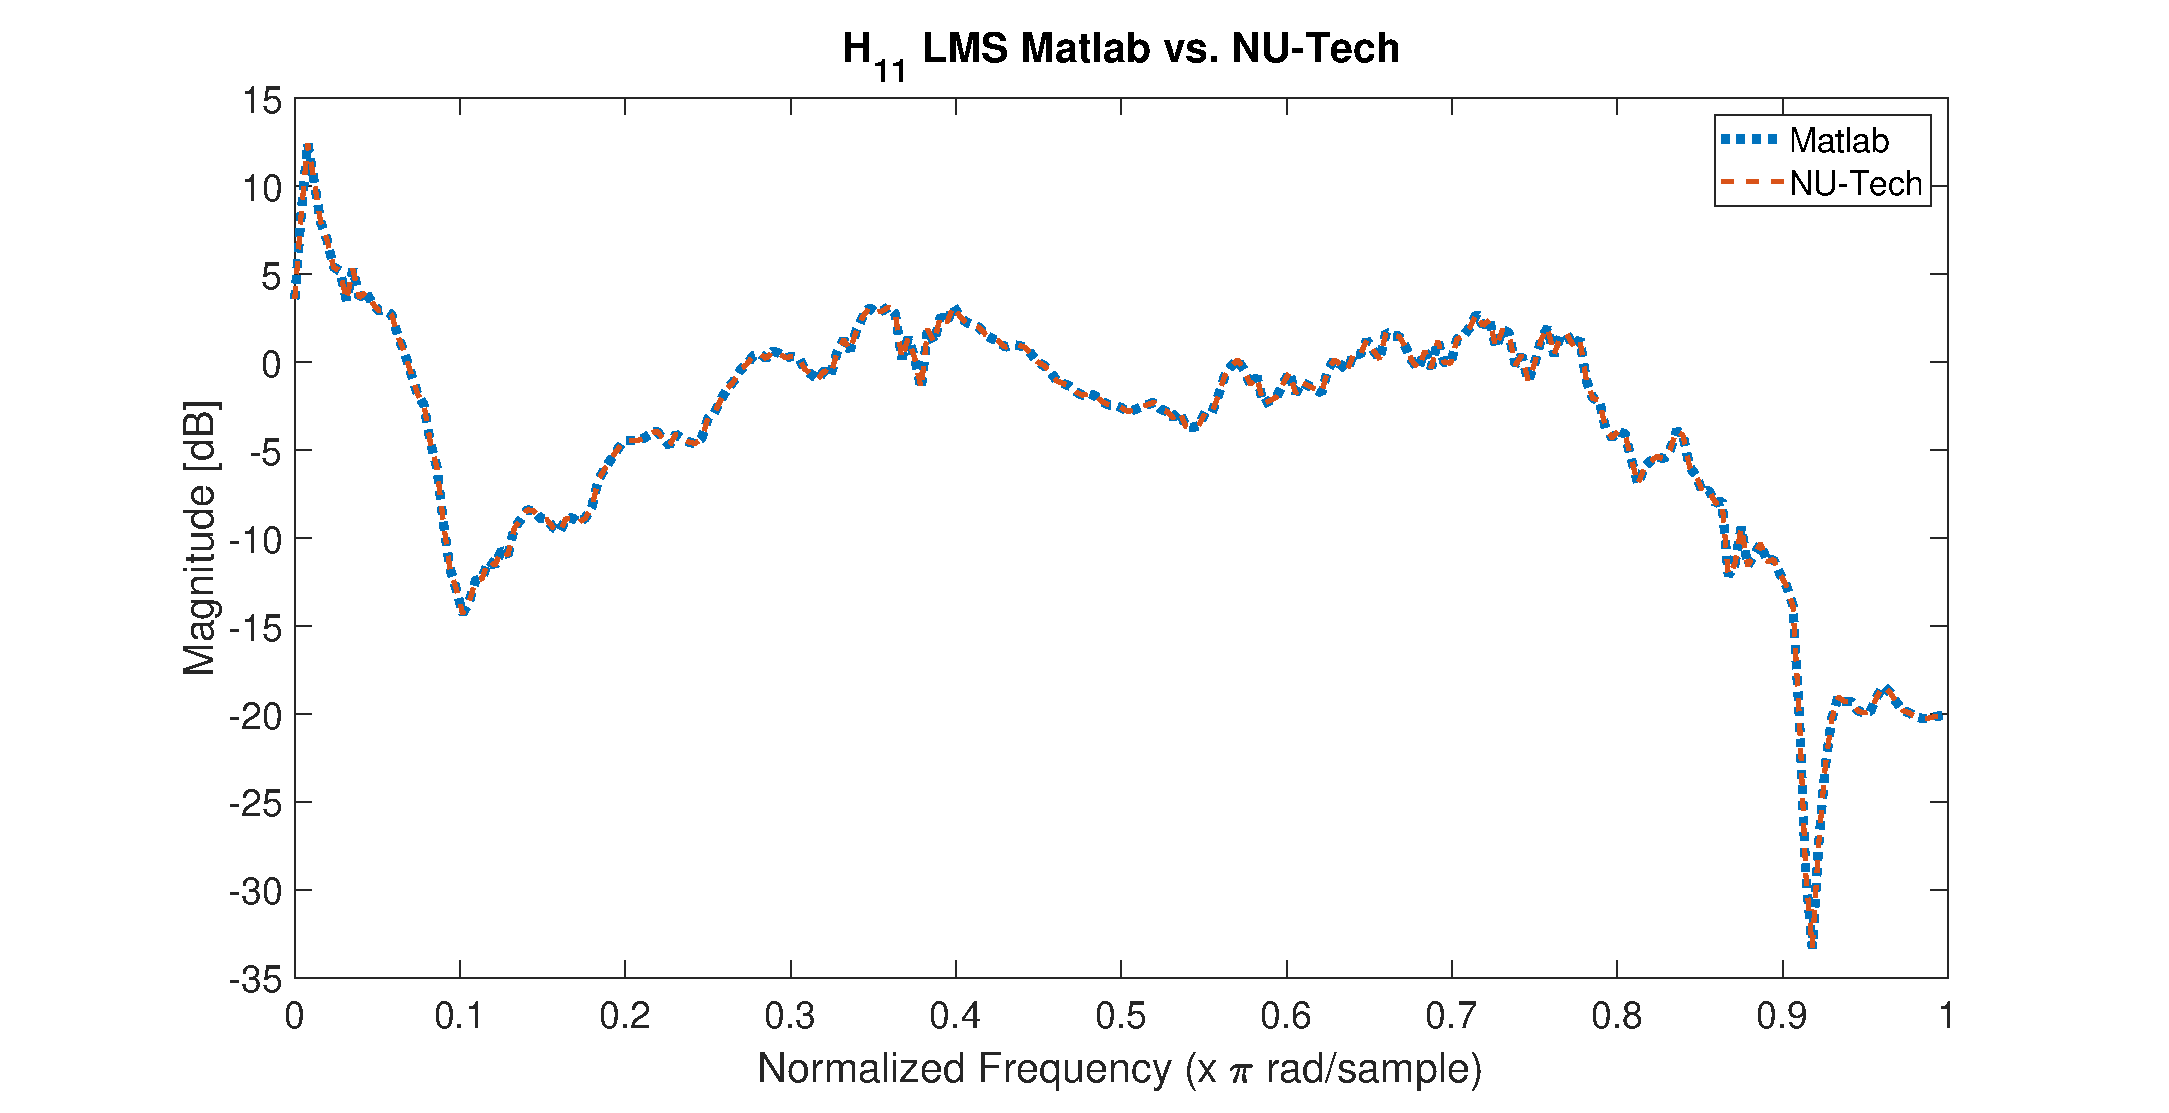
\includegraphics[width=1\textwidth]{Immagini/H11_LMS_matlab_nutech}
		\caption{}
		\label{fig:H11_LMS_matlab_nutech}
	\end{subfigure}
	\hfill
	\begin{subfigure}{.45\textwidth}
			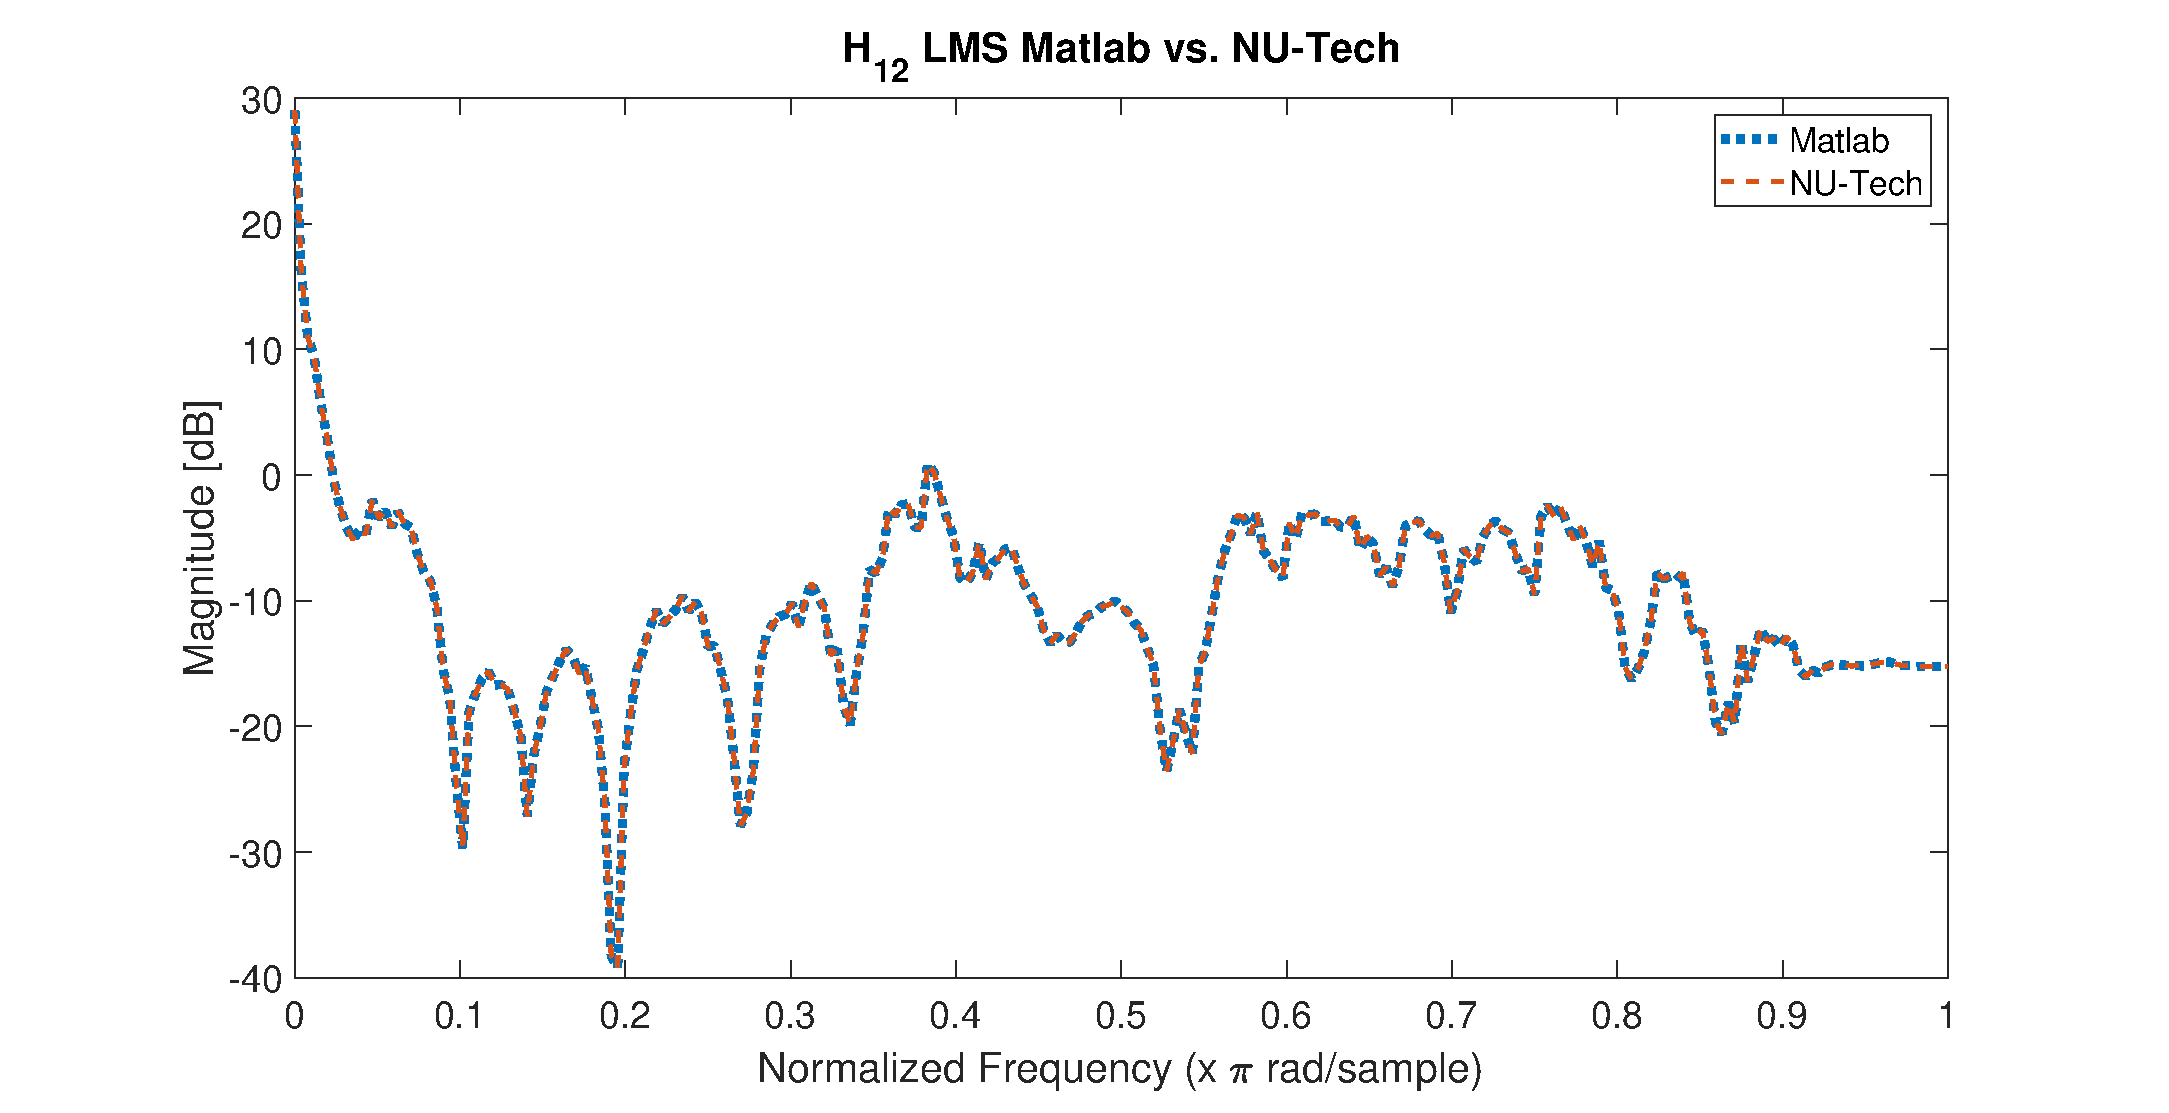
\includegraphics[width=1\textwidth]{Immagini/H12_LMS_matlab_nutech}
			\caption{}
			\label{fig:H12_LMS_matlab_nutech}
	\end{subfigure}
	\vfill
	\begin{subfigure}{.45\textwidth}
		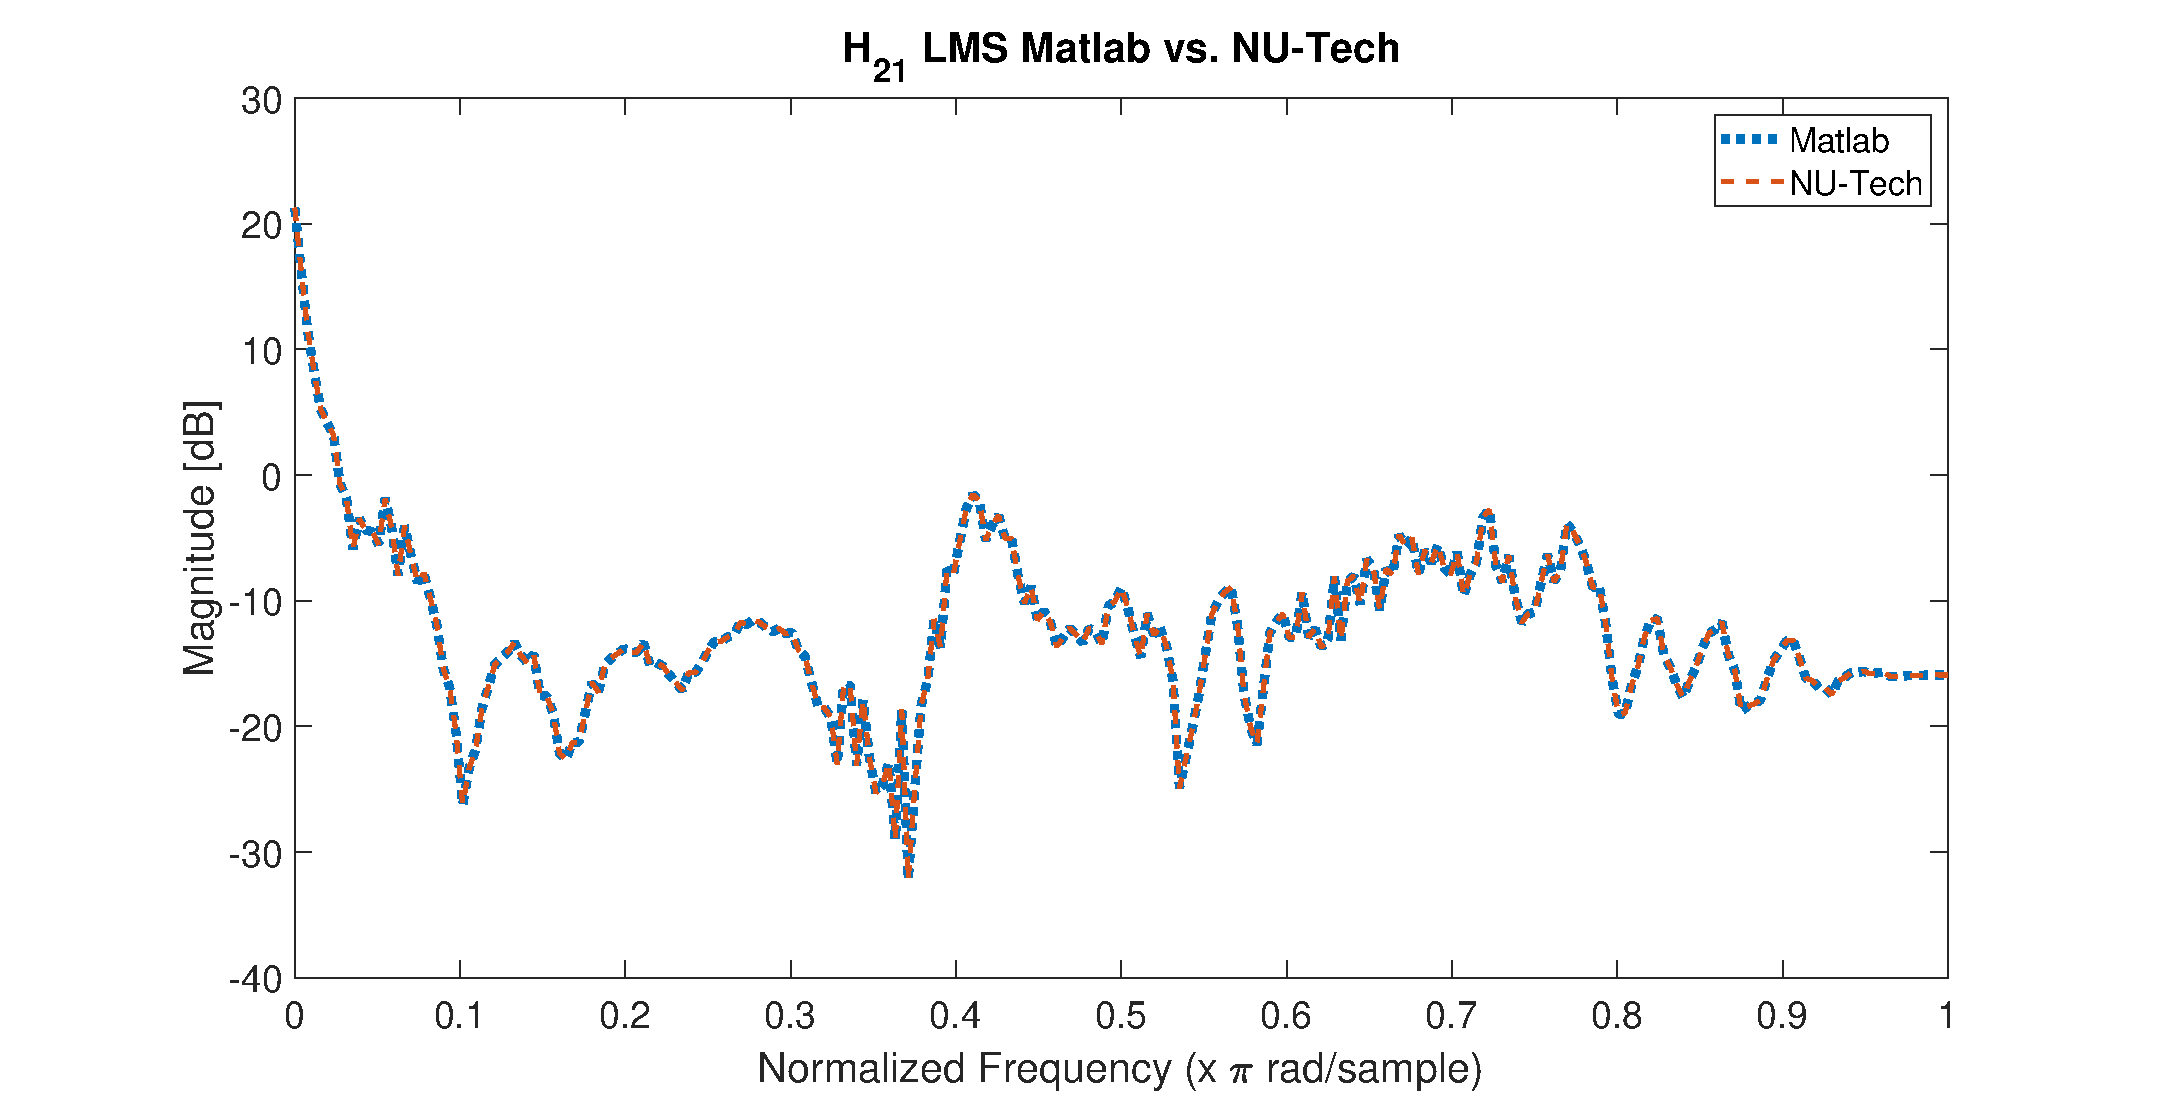
\includegraphics[width=1\textwidth]{Immagini/H21_LMS_matlab_nutech}
		\caption{}
		\label{fig:H21_LMS_matlab_nutech}
	\end{subfigure}
	\hfill
	\begin{subfigure}{.45\textwidth}
		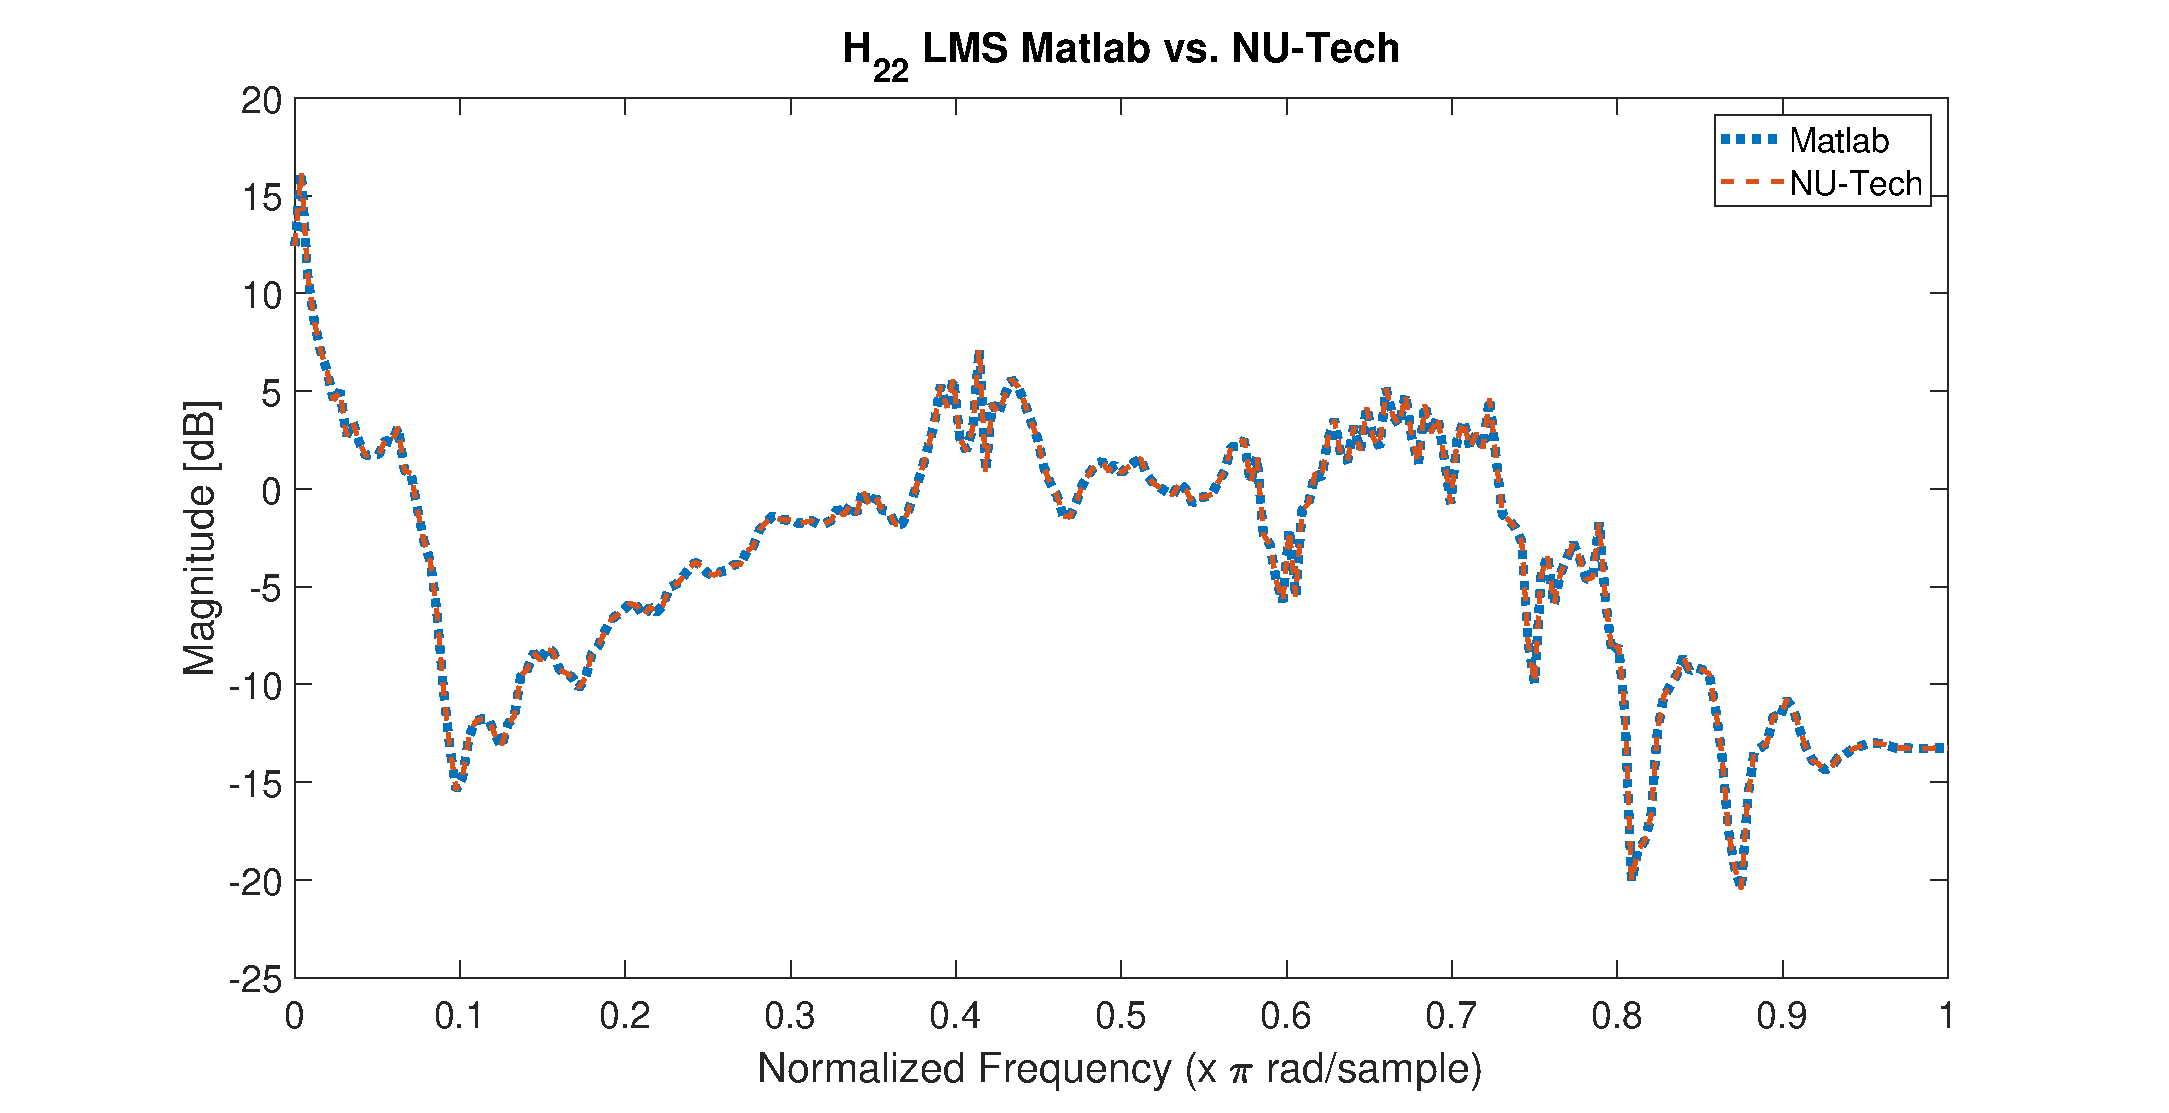
\includegraphics[width=1\textwidth]{Immagini/H22_LMS_matlab_nutech}
		\caption{}
		\label{fig:H22_LMS_matlab_nutech}
	\end{subfigure}
		\caption{Confronto dei filtri di cancellazione del crosstalk (a) $H_{11}$, (b) $H_{12}$, (c) $H_{21}$ e (d) $H_{22}$ in Matlab e in NU-Tech per l'algoritmo LMS.}
		\label{fig:confronto_filtri_matlab_nutech_lms}
\end{figure}
\end{frame}

\begin{frame}
\begin{figure}[h]
	\centering
	\begin{subfigure}{.45\textwidth}
		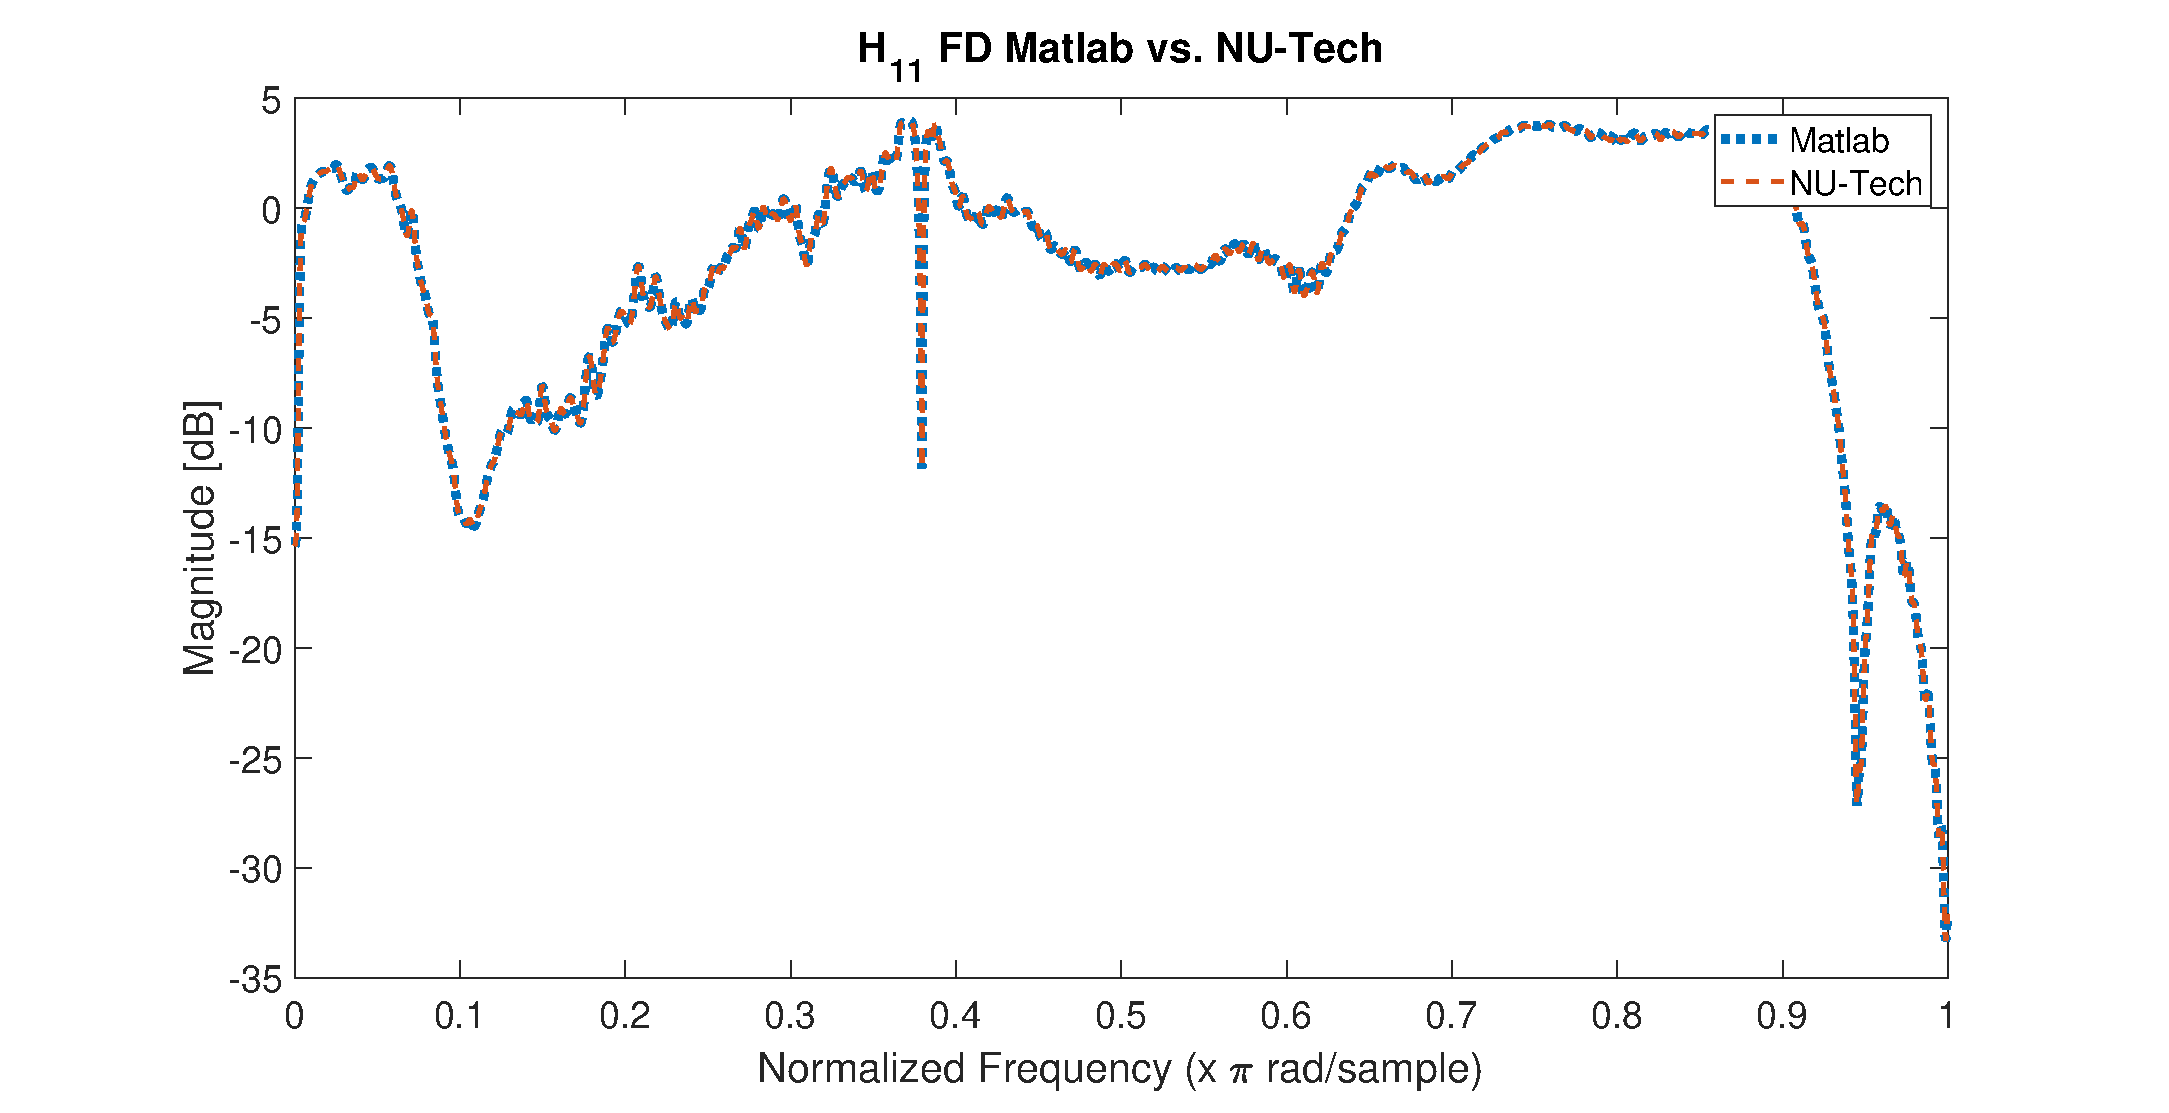
\includegraphics[width=1\textwidth]{Immagini/H11_FD_matlab_nutech}
		\caption{}
		\label{fig:H11_FD_matlab_nutech}
	\end{subfigure}
	\hfill
	\begin{subfigure}{.45\textwidth}
			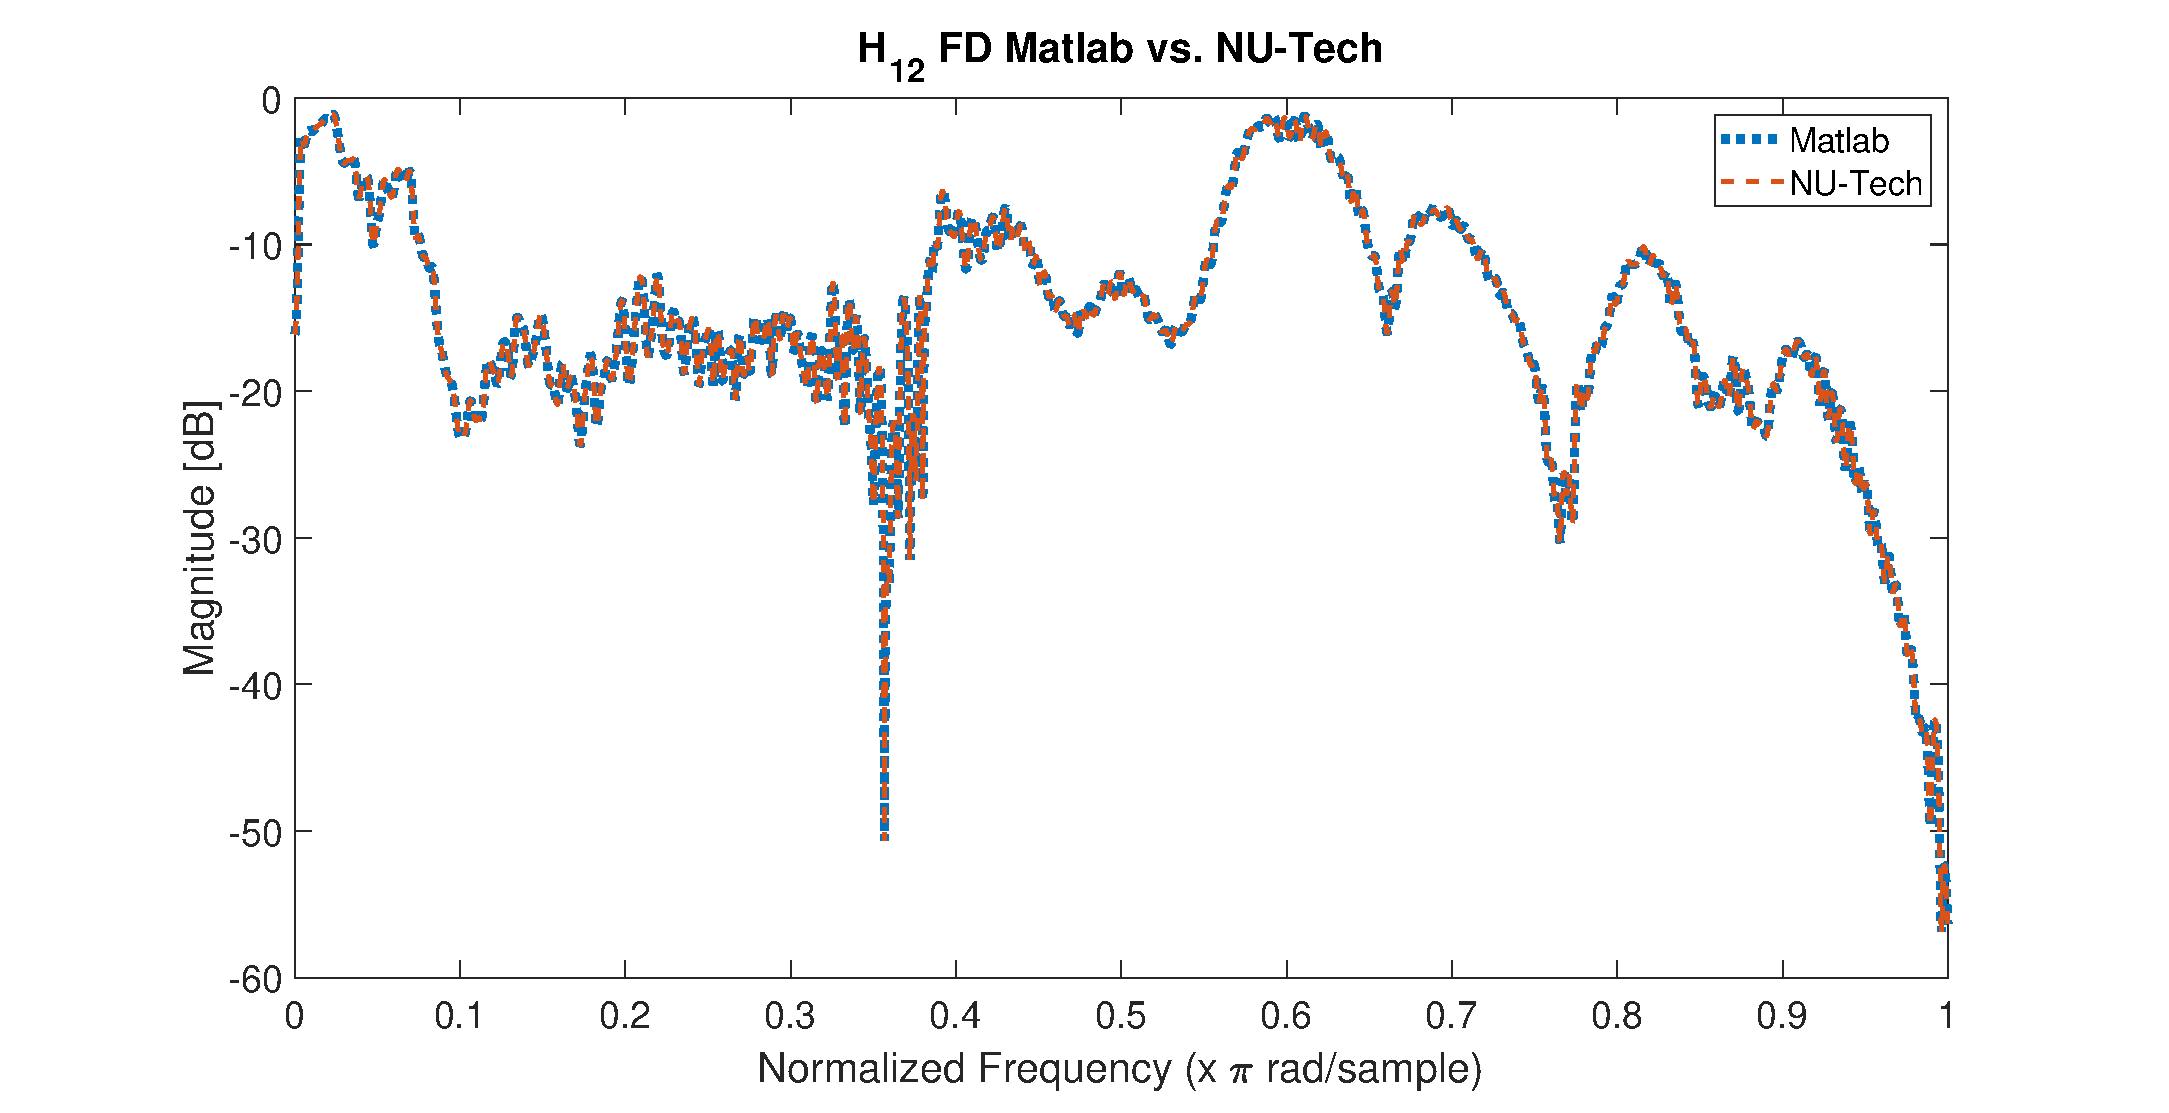
\includegraphics[width=1\textwidth]{Immagini/H12_FD_matlab_nutech}
			\caption{}
			\label{fig:H12_FD_matlab_nutech}
	\end{subfigure}
	\vfill
	\begin{subfigure}{.45\textwidth}
		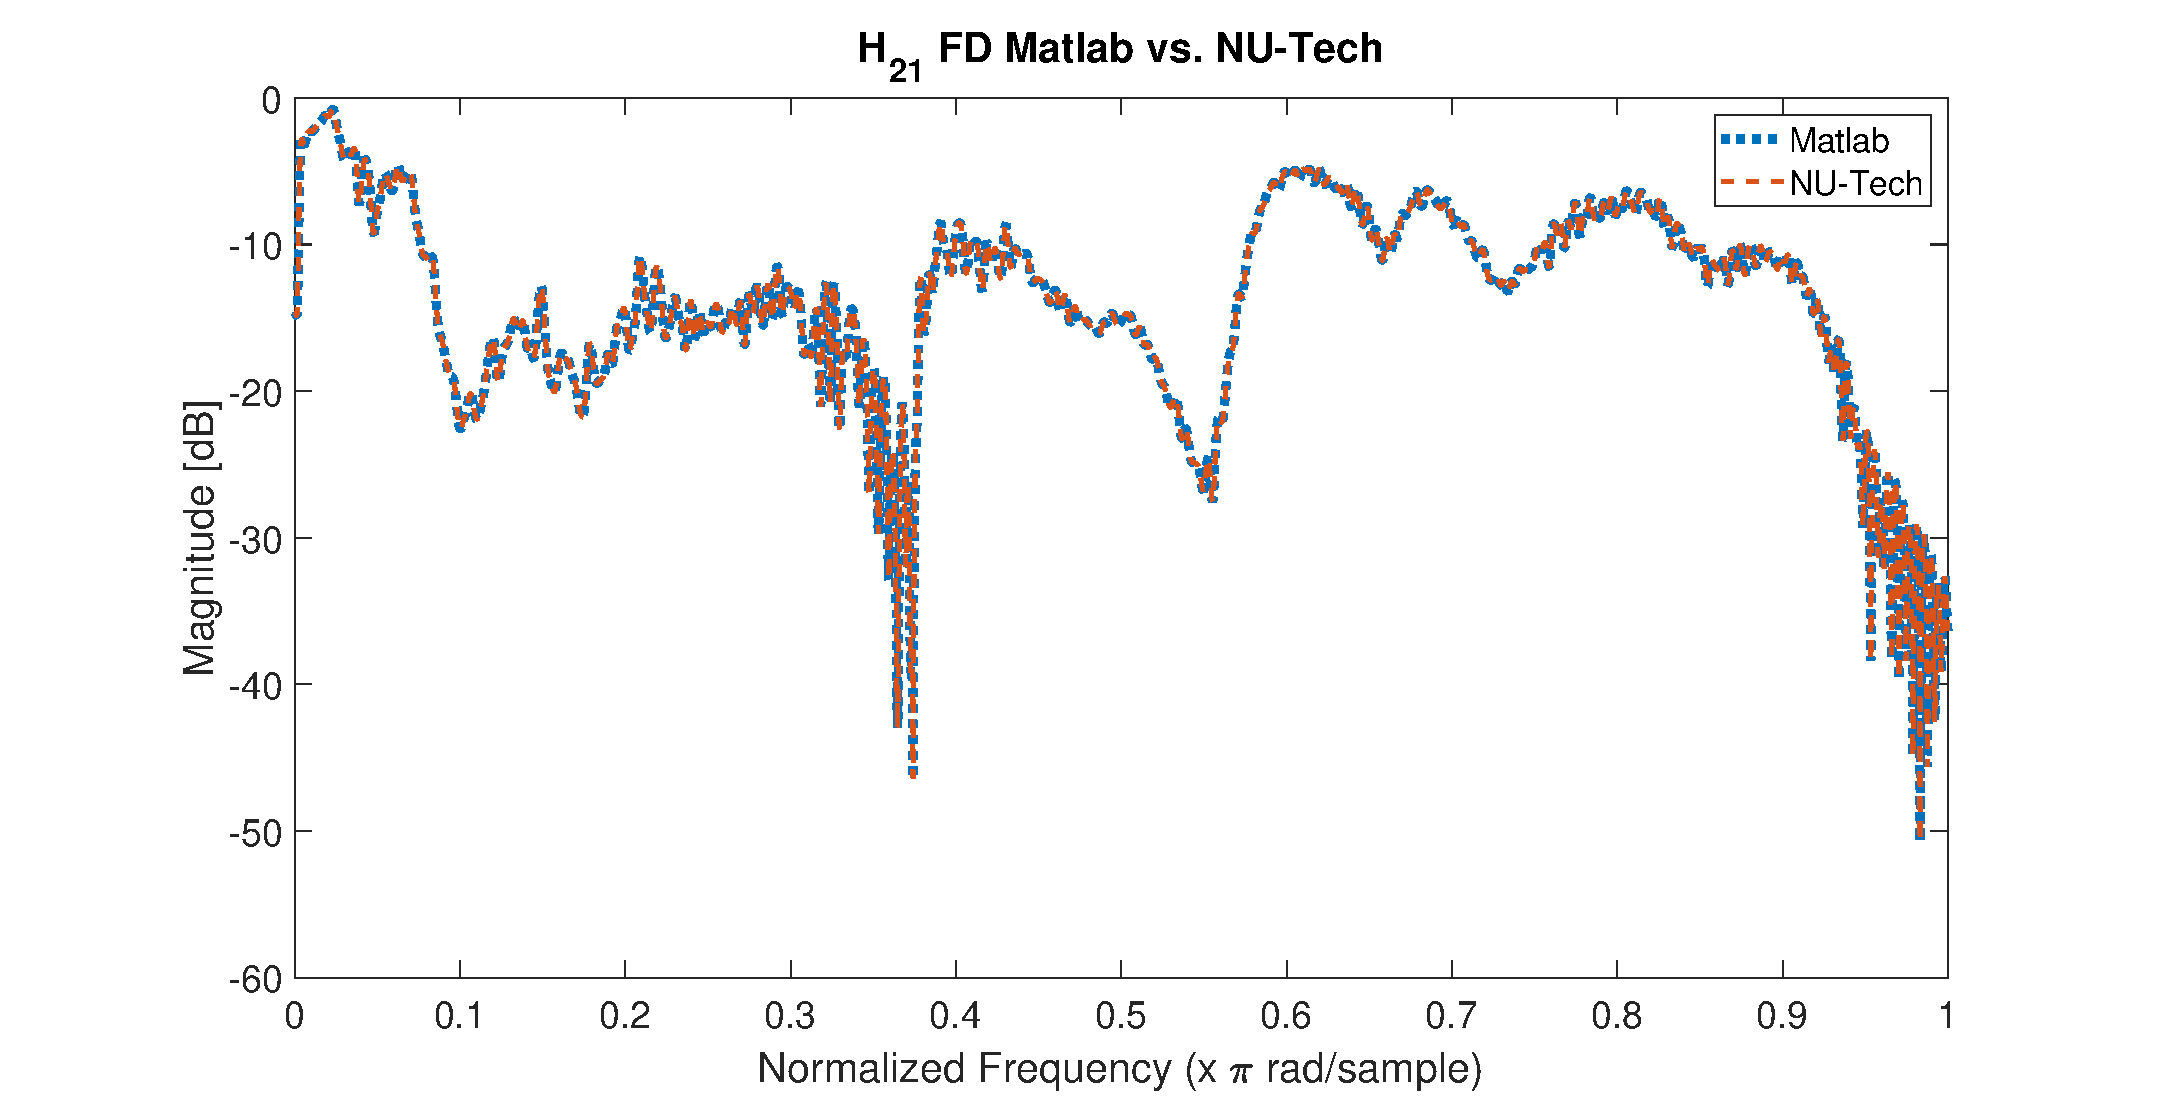
\includegraphics[width=1\textwidth]{Immagini/H21_FD_matlab_nutech}
		\caption{}
		\label{fig:H21_FD_matlab_nutech}
	\end{subfigure}
	\hfill
	\begin{subfigure}{.45\textwidth}
		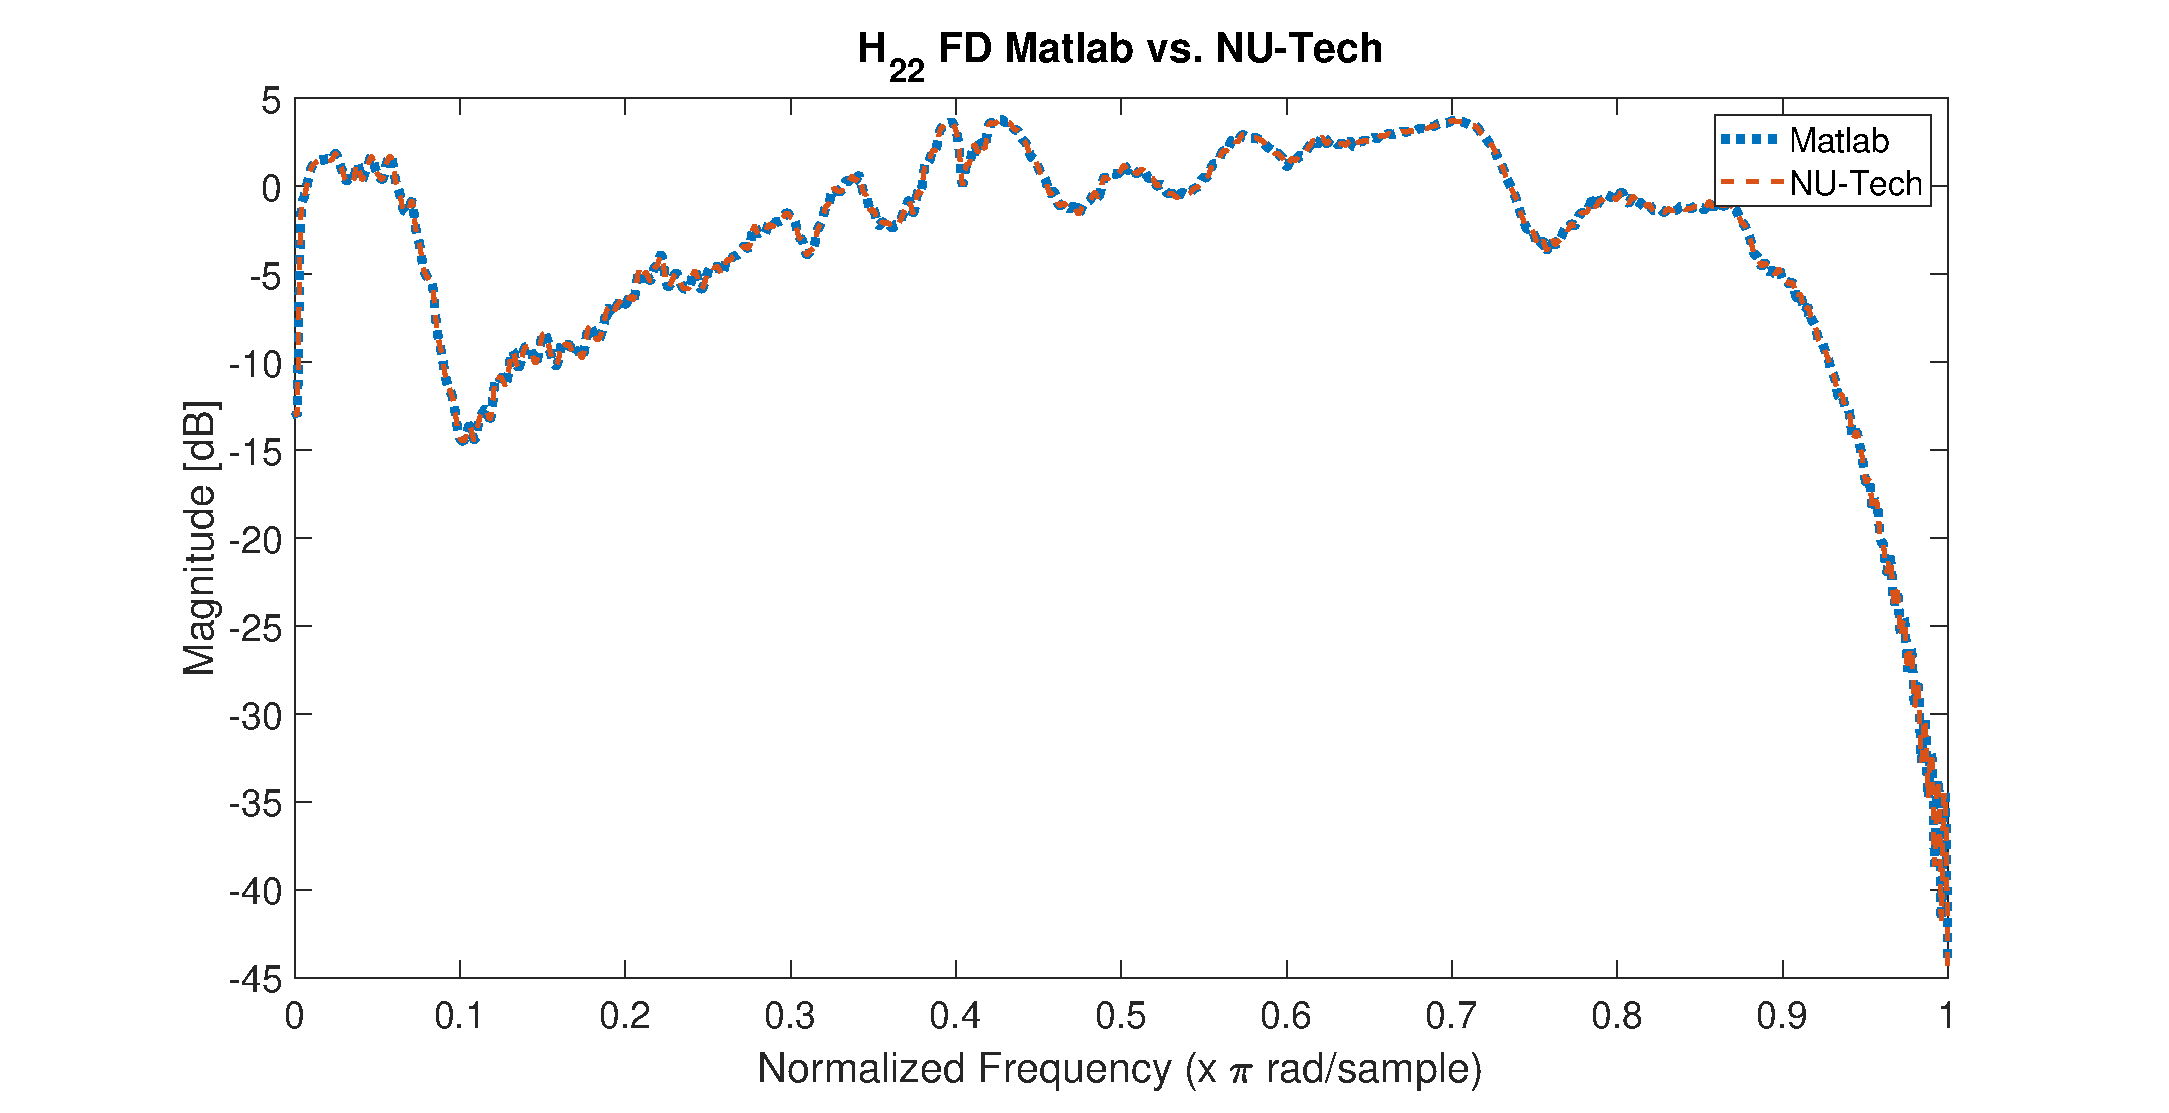
\includegraphics[width=1\textwidth]{Immagini/H22_FD_matlab_nutech}
		\caption{}
		\label{fig:H22_FD_matlab_nutech}
	\end{subfigure}
		\caption{Confronto dei filtri di cancellazione del crosstalk (a) $H_{11}$, (b) $H_{12}$, (c) $H_{21}$ e (d) $H_{22}$ in Matlab e in NU-Tech per l'algoritmo Fast Deconvolution.}
		\label{fig:confronto_filtri_matlab_nutech_fd}
\end{figure}
\end{frame}
\nocite{*}
\section*{Bibliografia}
\begin{frame}[allowframebreaks]
\frametitle{Bibliografia}
\tiny\printbibliography[heading=none]
\end{frame}

\end{document}